% Supplementary material for paper.tex. Build: make supplement
\documentclass[11pt,a4paper]{article}

\usepackage{iftex}
\ifPDFTeX
\usepackage[T1]{fontenc}
\usepackage{lmodern}
\else
\usepackage{fontspec}
\fi
\usepackage[a4paper,margin=2.4cm]{geometry}
\usepackage{amsmath}
\usepackage{graphicx}
\usepackage{booktabs}
\usepackage{makecell}
\usepackage{array}
\usepackage[font=small,labelfont=bf]{caption}
\usepackage{enumitem}
\usepackage{fancyhdr}
\usepackage[hidelinks]{hyperref}
\usepackage{xurl}
\usepackage{tocloft}
\setlength{\cftsecnumwidth}{2.6em}

\newcommand{\Mw}{$M_\mathrm{w}$}
\newcommand{\stalta}{STA/LTA}
\newcommand{\VP}{$V_\mathrm{P}$}
\newcommand{\VS}{$V_\mathrm{S}$}
\newcommand{\tool}[1]{\nolinkurl{#1}}
% A note under a table, as in the paper.
\newcommand{\tablenote}[1]{\par\vspace{4pt}%
  \begin{minipage}{\linewidth}\footnotesize\textit{Note.} #1
\end{minipage}}

\setlist{itemsep=2pt,topsep=4pt}
\setlength{\emergencystretch}{1.5em}
\renewcommand{\arraystretch}{1.15}
\renewcommand{\thesection}{S\arabic{section}}
\renewcommand{\thetable}{S\arabic{table}}
% One table per section, so that Table Sn belongs to Section Sn.
\newcommand{\panel}[1]{\par\smallskip\noindent\textbf{(#1)}\enskip}

\pagestyle{fancy}
\fancyhf{}
\renewcommand{\headrulewidth}{0pt}
\fancyfoot[C]{\thepage}
\renewcommand{\thepage}{S\arabic{page}}

\title{Supplementary material for\\[4pt]
  \large A Self-Contained Real-Time Detection Pipeline and an Operating-Point Replay
Protocol Applied to Turkish Broadband Stations}
\author{H. O\u{g}uz Bolat, Sibel \c{C}imen, B\"ulent Bolat, T\"ulay Y\i{}ld\i{}r\i{}m}

\date{29 October 2026}
\begin{document}
\maketitle
\thispagestyle{fancy}

\noindent Every number below was produced by a tool in the pipeline's repository
(\url{https://github.com/hogib/ayzek}, \tool{tools/}) or in the offline
evaluation code, and the command is named with each table. The AFAD waveforms
cannot be redistributed; the KOERI datasets are attached to the pipeline's
releases.

\tableofcontents

% ---------------------------------------------------------------------------
\section{Stations and quiet windows}\label{s:stations}

Table~\ref{t:stations}a lists the stations of the replays. All TU stations
record HH channels at 100~Hz. No TU station contributed a window to the
training, validation or test sets of the pipeline's detector; the KOERI datasets
do not share this guarantee, and the role of each KO station in the detector's
station split is given. The replay of the S\i{}nd\i{}rg\i{} 30-minute window uses DEMI, MANT and BAND only.
The eleventh station of the continuous archive, GCAM, is in none of the replays and is
not listed.

Table~\ref{t:stations}b lists the 23 AFAD quiet windows, in which no cataloged event lies within 250~km of any of the eight stations during the window or for 30~min
on either side of it. Each window is replayed on its own; its first 30~min warm
the noise baseline and the \stalta{} and are not scored.

\begin{table}[htbp]
  \centering\small
  \caption{Stations and quiet windows.}\label{t:stations}
  \panel{a} Stations. Datasets: S30, S\i{}nd\i{}rg\i{} 30~min (tuning);
  Mar, Marmara (tuning); S61, S\i{}nd\i{}rg\i{} \Mw{}~6.1 (held out); Sim, Simav
  \Mw{}~4.8 (second held out); Q, the AFAD quiet windows; and the three KOERI
  datasets.\par\smallskip
  \begin{tabular}{@{}llrrll@{}}
    \toprule
    Station & Net. & Lat. & Lon. & Datasets & Detector split \\
    \midrule
    ARNA & TU & 41.3470 & 28.6838 & Mar & none \\
    BAND & TU & 40.3553 & 28.0992 & S30, Mar, Sim, Q & none \\
    CATL & TU & 41.3407 & 28.3561 & Mar & none \\
    CMH  & TU & 40.0115 & 27.9703 & S61, Q & none \\
    DEMI & TU & 39.0428 & 28.7162 & S30, Mar, S61, Sim & none \\
    ELBA & TU & 41.1469 & 28.4307 & Mar, Q & none \\
    KAND & TU & 41.0943 & 30.1922 & S61, Sim, Q & none \\
    KURT & TU & 40.5905 & 29.2092 & Sim & none \\
    KIRK & TU & 41.7817 & 27.0972 & Mar, S61, Q & none \\
    MANT & TU & 38.4908 & 28.5579 & S30, Mar, Sim, Q & none \\
    SEMS & TU & 40.8710 & 29.7391 & Mar, S61, Q & none \\
    VIZE & TU & 41.5785 & 27.8400 & S61, Sim, Q & none \\
    \addlinespace
    ARMT & KO & 40.5683 & 28.8660 & marmara\_ko & test \\
    BGKT & KO & 41.1810 & 28.7730 & marmara\_ko & training \\
    BOTS & KO & 40.9902 & 27.9810 & marmara\_ko & training \\
    CTKS & KO & 41.2373 & 28.5072 & marmara\_ko & training \\
    DKL  & KO & 39.0713 & 26.9053 & demo\_ko, quiet\_ko & training \\
    EDC  & KO & 40.3465 & 27.8618 & marmara\_ko & validation \\
    GEDZ & KO & 39.0445 & 29.4105 & quiet\_ko & test \\
    KCTX & KO & 40.2627 & 28.3353 & demo\_ko & training \\
    KULA & KO & 38.5145 & 28.6607 & demo\_ko, quiet\_ko & test \\
    MRMT & KO & 40.6090 & 27.5832 & marmara\_ko & training \\
    SIMA & KO & 39.0833 & 28.9825 & demo\_ko, quiet\_ko & validation \\
    SLVT & KO & 41.2300 & 28.2100 & marmara\_ko & training \\
    TKR  & KO & 40.9902 & 27.5357 & marmara\_ko & test \\
    TVSB & KO & 39.4497 & 29.4615 & demo\_ko, quiet\_ko & training \\
    YAYO & KO & 39.6113 & 27.0726 & demo\_ko, quiet\_ko & training \\
    \bottomrule
  \end{tabular}

  \bigskip
  \panel{b} AFAD quiet windows: scored interval (UTC; $^{+1}$, the next day),
  scored hours, stations (St.), and the alarms of the learned detector (L) and of
  the \stalta{} at equal unmatched alarms (S).\par\smallskip
  {\footnotesize\setlength{\tabcolsep}{4pt}
    \begin{tabular}[t]{@{}lccrrrr@{}}
      \toprule
      Date & From & To & Hours & St. & L & S \\
      \midrule
      2024-05-22 & 19:54 & 02:05$^{+1}$ & 6.19 & 8 & 1 & 46 \\
      2024-05-23 & 04:22 & 07:48 & 3.43 & 8 & 1 & 11 \\
      2024-05-23 & 21:51 & 01:17$^{+1}$ & 3.43 & 8 & 2 & 28 \\
      2024-05-24 & 15:20 & 19:24 & 4.07 & 8 & 0 & 16 \\
      2024-05-26 & 00:31 & 03:48 & 3.27 & 8 & 0 & 17 \\
      2024-05-29 & 07:08 & 10:12 & 3.06 & 7 & 1 & 16 \\
      2024-05-30 & 15:45 & 20:57 & 5.21 & 7 & 1 & 14 \\
      2024-06-02 & 23:30 & 07:21$^{+1}$ & 7.85 & 8 & 2 & 30 \\
      2024-06-05 & 02:10 & 11:46 & 9.60 & 8 & 2 & 52 \\
      2024-06-06 & 10:54 & 13:56 & 3.04 & 8 & 0 & 11 \\
      2024-06-06 & 15:26 & 20:41 & 5.24 & 8 & 0 & 14 \\
      2024-06-09 & 12:40 & 18:05 & 5.41 & 8 & 2 & 11 \\
      \bottomrule
    \end{tabular}\hfill
    \begin{tabular}[t]{@{}lccrrrr@{}}
      \toprule
      Date & From & To & Hours & St. & L & S \\
      \midrule
      2024-12-25 & 16:47 & 21:06 & 4.31 & 8 & 0 & 2 \\
      2025-01-04 & 20:37 & 23:29 & 2.87 & 8 & 0 & 1 \\
      2025-02-24 & 12:13 & 15:23 & 3.15 & 7 & 0 & 4 \\
      2025-02-26 & 16:55 & 20:25 & 3.50 & 8 & 2 & 10 \\
      2025-02-26 & 21:55 & 02:58$^{+1}$ & 5.06 & 8 & 0 & 1 \\
      2025-02-27 & 12:27 & 16:26 & 3.97 & 8 & 1 & 6 \\
      2025-02-27 & 18:41 & 00:14$^{+1}$ & 5.55 & 8 & 0 & 5 \\
      2025-03-02 & 14:54 & 17:51 & 2.94 & 7 & 1 & 8 \\
      2025-03-03 & 18:29 & 22:58 & 4.49 & 7 & 0 & 0 \\
      2025-03-04 & 19:00 & 22:12 & 3.19 & 7 & 0 & 6 \\
      2025-03-07 & 20:22 & 00:20$^{+1}$ & 3.96 & 7 & 0 & 14 \\
      \midrule
      total & & & 102.79 & & 16 & 323 \\
      \bottomrule
  \end{tabular}}
\end{table}

\noindent Reproduction: \tool{tools/extract_quiet.py} selects the windows, and
stage~6 of \tool{tools/reproduce_all.sh} replays them with both detectors. Station coordinates:
\tool{models/stations.csv} and each KO dataset's \tool{stations.json}.

% ---------------------------------------------------------------------------
\clearpage
\section{Verification and the data path}\label{s:verification}

\paragraph{Numerical agreement.} Every network of the pipeline is a
transcription of its PyTorch module and reads the same \texttt{state\_dict}.
The test suite (15 tests, \tool{meson test}) compares each stage with its
reference on real waveforms (Table~\ref{t:verification}a). Window conditioning
runs in double precision as SciPy does; the residual of the cleaned signal is
the rounding of an eighth-order IIR filter in transfer-function form. The
picker's picks are identical to PyTorch's. The aarch64 build passes the same
suite under emulation and, on a Raspberry~Pi~4, raises the same alarms at the
same times with the same locations as the x86 build on the KOERI datasets.

\paragraph{Undecodable records.} During the \Mw{}~6.2 of 2025-04-23, the
dataloggers at CATL (57~km) and ARNA (68~km) switched from Steim-2 compression
to uncompressed 32-bit integer records (CATL little-endian, ARNA big-endian);
ELBA, at 38~km, did not. A decoder that accepted only Steim-2 rejected all of them, 104 records at CATL and 155 at ARNA, at 09:49--09:51 and 10:02--10:03 UTC, and the two stations therefore recorded no detection of the strongest shaking. The
pipeline now decodes integer records in either byte order (both files decode
bit-exactly against ObsPy) and reports, with the reason, any record it cannot
decode. A scan of the whole archive (its 13 stations, the eleven of the continuous
archive and ARNA and CATL; 283 chunks, 398 million records, 2024--2026) found 304 non-Steim-2 records, all at ARNA and CATL on
that day between 09:49 and 12:13 UTC.

\paragraph{Sample loss under load.} The pipeline dates a sample by its position
in a ring of $2^{17}$ samples (21.8~min at 100~Hz) per component. An earlier
implementation dropped the samples it could not hold when a ring was full. A
network-wide archive outage of 2{,}095.6--2{,}103.4~s per component (1.60 times the ring, on all 27 components of nine stations at once) exposed the defect. Because position is ring index plus base, a dropped sample does not leave a hole but moves every later sample of that component earlier, and after the outage the three components of a station no longer describe the same instant.
In the current pipeline, writes never wait and never drop. What does not fit is queued per component, and a gap is queued as a count, so an outage of any length costs no memory. Table~\ref{t:verification}b repeats the Marmara replay
with a 25-minute hole cut into the record of all eight stations, ending 49~min
before the \Mw{}~6.2. With the current pipeline the hole changes nothing but
the two single-station detections inside it; with the earlier one, 329{,}439
dropped samples cost 15 of the 44 detections and the \Mw{}~5.9. The 11.6-hour
window containing the outage is replayed without a stall or a drop, and
yields exactly the windows, triggers, picks and alarms of the two runs split
around it (711{,}760 windows, 86 triggers and the same five alarms to the
hundredth of a second); only the windows rejected for crossing the gap differ.

\begin{table}[htbp]
  \centering\footnotesize\setlength{\tabcolsep}{4pt}
  \caption{Verification.}\label{t:verification}
  \panel{a} Largest difference from the reference, on real windows.\par\smallskip
  \begin{tabular}{@{}llr@{}}
    \toprule
    Stage & Reference & Largest difference \\
    \midrule
    cleaned window (detrend, taper, 1--45~Hz zero-phase) & SciPy & $1.1\times10^{-8}$ relative \\
    standardized window (float) & NumPy & $1.9\times10^{-9}$ absolute \\
    detector: convolutional stack & PyTorch & $3.8\times10^{-6}$ \\
    detector: BiLSTM & PyTorch & $1.3\times10^{-6}$ \\
    detector: attention & PyTorch & $9.5\times10^{-7}$ \\
    detector: logit & PyTorch & $6.0\times10^{-7}$ \\
    detector: ensemble probability & PyTorch & identical to 5 decimals \\
    picker: logits & PyTorch & $5.7\times10^{-6}$ (picks identical) \\
    \stalta{}: filter coefficients & SciPy \texttt{butter(4, sos)} & $2\times10^{-16}$ \\
    \stalta{}: filtered trace (peak $9\times10^{5}$ counts) & SciPy & $10^{-8}$ counts \\
    \stalta{}: ratio, vertical & ObsPy \texttt{recursive\_sta\_lta} & $5\times10^{-14}$ relative \\
    \stalta{}: ratio, three components & ObsPy & $8\times10^{-14}$ relative \\
    \bottomrule
  \end{tabular}

  \bigskip
  \panel{b} Marmara replay (57 cataloged events), records starting
  08:35--09:00~UTC removed from all eight stations.\par\smallskip
  \begin{tabular}{@{}lccc@{}}
    \toprule
    & Unbroken, current & Gap, current & Gap, earlier \\
    \midrule
    stalls / samples dropped & 0 / 0 & 0 / 0 & 112 / 329{,}439 \\
    alarms raised & 68 & 68 & 76 \\
    alarms matching a cataloged event & 44 & 44 & 29 \\
    alarms without one & 24 & 24 & 47 \\
    cataloged events detected & 44 & 44 & 29 \\
    \Mw{}~6.2 alarm & +11.0~s, ARNA+ELBA & identical & two alarms, CATL+ELBA \\
    \Mw{}~5.9 alarm & +12.5~s & identical & not raised \\
    \bottomrule
  \end{tabular}
\end{table}

\noindent Reproduction: \tool{tests/} (\tool{test_dsp}, \tool{test_models},
\tool{test_stalta}, \tool{test_steim}, \tool{test_writer}, \ldots);
\tool{tools/scan_encodings.py} for the archive; the gapped replays are
described in the repository's \tool{docs/impl/05-pipeline.md}.

% ---------------------------------------------------------------------------
\clearpage
\section{Quiet-window detections per station}\label{s:perstation}

Station detections on the AFAD quiet windows, after the lead-in of each
window, with detections within 40~s at one station counted once. The rate is
per day of the scored hours of the windows the station is part of; alarms are
those the station declared. KIRK's detections under the learned detector are
the instrumental pulse described in the main text (218 of the 225 at one phase
of a 10-minute cycle locked to UTC). Under \stalta{}, CMH and KIRK dominate,
and KAND, with 16 detections under the learned detector, does not trigger at
all.

\begin{table}[htbp]
  \centering\small
  \caption{Detections and alarms per station on 102.8~h of AFAD quiet data.}\label{t:perstation}
  \begin{tabular}{@{}lrrrrrrr@{}}
    \toprule
    & & \multicolumn{3}{c}{Learned detector} & \multicolumn{3}{c}{\stalta{}, equal unmatched alarms} \\
    \cmidrule(lr){3-5}\cmidrule(l){6-8}
    Station & Hours & Detections & Per day & Alarms & Detections & Per day & Alarms \\
    \midrule
    BAND & 102.8 & 31  & 7.2  & 9  & 172 & 40.2  & 50  \\
    CMH  & 102.8 & 30  & 7.0  & 6  & 993 & 231.9 & 227 \\
    ELBA & 102.8 & 1   & 0.2  & 0  & 30  & 7.0   & 4   \\
    KAND & 88.2  & 16  & 4.4  & 2  & 0   & 0.0   & 0   \\
    KIRK & 102.8 & 225 & 52.5 & 10 & 804 & 187.7 & 232 \\
    MANT & 94.5  & 15  & 3.8  & 1  & 83  & 21.1  & 39  \\
    SEMS & 99.6  & 33  & 7.9  & 3  & 153 & 36.9  & 56  \\
    VIZE & 102.8 & 3   & 0.7  & 1  & 146 & 34.1  & 38  \\
    \midrule
    total & & 354 & & 16 alarms & 2{,}381 & & 323 alarms \\
    \bottomrule
  \end{tabular}
\end{table}

\noindent Reproduction: \tool{python3 tools/quiet_stations.py --runs
learned=data/runs/quiet100 stalta=data/runs/quiet100_stalta}. An alarm is
declared by two stations, so the per-station alarm counts sum to twice the
alarms.

% ---------------------------------------------------------------------------
\clearpage
\section{Computational cost}\label{s:cost}

Each stage was timed with the pipeline's benchmark (\tool{ayzek_bench}) on
synthetic seeded input, after a warm-up, for at least one second and ten
calls; inference time does not depend on the sample values. The x86 machine is
an AMD Ryzen~5 5600 (6 cores, 12 threads), release build with GCC~16.2, idle;
the Raspberry~Pi~4 (Cortex-A72, 4 cores at 1.8~GHz) runs the static aarch64
build with NEON kernels, each group starting below 55~\textdegree C with the
clock held at 1.8~GHz throughout. A station needs one window every 0.5~s; the
capacity is the stations whose windows one to all cores sustain. The published
models of main-text Section~4.3 were timed separately under PyTorch, one forward
pass per 0.5~s step and station as the evaluation ran them.

\begin{table}[htbp]
  \centering\small
  \caption{Cost per stage (median) and real-time capacity.}\label{t:cost}
  \panel{a} Per call.\par\smallskip
  \begin{tabular}{@{}lrr@{}}
    \toprule
    Stage & Ryzen 5 5600 & Raspberry Pi 4 \\
    \midrule
    condition a 6~s window & 0.04~ms & 0.14~ms \\
    detector, one network & 1.7~ms & 11.8~ms \\
    detector ensemble, three networks & 5.2~ms & 36.3~ms \\
    \stalta{}, 50 samples (one 0.5~s step) & 0.0005~ms & 0.0019~ms \\
    per 0.5~s step and station (conditioning, ensemble, \stalta{}) & 5.2~ms & \\
    picker, one 60~s window & 12.0~ms & 75.7~ms \\
    \addlinespace
    EQTransformer, one pass (60~s input), PyTorch, one thread & 9.1~ms & \\
    PhaseNet, one pass (30~s input), PyTorch, one thread & 1.6~ms & \\
    \bottomrule
  \end{tabular}

  \bigskip
  \panel{b} Stations whose detector windows the cores sustain.\par\smallskip
  \begin{tabular}{@{}lrr@{}}
    \toprule
    Threads & Ryzen 5 5600 & Raspberry Pi 4 \\
    \midrule
    1 & 95 & 14 \\
    4 & 379 & 52 \\
    12 & 653 & \\
    \bottomrule
  \end{tabular}
\end{table}

\noindent Reproduction: \tool{build-release/bench/ayzek_bench --group
stages,capacity}; \tool{tools/bench_pi.sh} on the board; results in the
repository's \tool{bench/results/models/}.

% ---------------------------------------------------------------------------
\clearpage
\section{Station subsets and alert time}\label{s:subsets}

The Marmara replay was recorded once (\tool{ayzek --record}) and its network
stage rerun for all 247 subsets of two to eight of its stations
(\tool{tools/network_subsets}), which gives the same result as replaying each
subset. Every subset declares the \Mw{}~6.2, and the best subset of every size
alerts at 11.0~s. Table~\ref{t:subsets}a gives the best subset per size and
Table~\ref{t:subsets}b the mean change when a station is added to a subset
without it. The four stations within 70~km each shorten the \Mw{}~6.2 alert by
about 7~s; SEMS and CATL add the most declared events and also the most
declared events without a catalog counterpart.

Against a geometric model in which the alert is the P travel time to the
subset's second-nearest station plus a latency, the observed alerts of the 247
subsets give a latency of median 2.05~s (interquartile range 0.58--2.77~s) and
a rank correlation of 0.71 between predicted and observed alert. The largest
residuals, 5.7~s, are the subsets in which KIRK (140~km) is the second station, because KIRK stays below the 0.9 plateau for the \Mw{}~6.2 and declares through the persistence branch.

\begin{table}[htbp]
  \centering\footnotesize\setlength{\tabcolsep}{4pt}
  \caption{Station subsets of the Marmara replay (57 cataloged events).}\label{t:subsets}
  \panel{a} Best subset per size, by the \Mw{}~6.2 alert.\par\smallskip
  \begin{tabular}{@{}rlccc@{}}
    \toprule
    $k$ & Stations & \Mw{}~6.2 alert & Events declared & Without catalog event \\
    \midrule
    2 & ARNA, ELBA & 11.0~s & 19 & 1 \\
    3 & ARNA, ELBA, SEMS & 11.0~s & 37 & 4 \\
    4 & ARNA, ELBA, KIRK, SEMS & 11.0~s & 41 & 8 \\
    5 & ARNA, CATL, ELBA, KIRK, SEMS & 11.0~s & 44 & 21 \\
    6 & ARNA, BAND, DEMI, ELBA, KIRK, SEMS & 11.0~s & 44 & 14 \\
    7 & all but CATL & 11.0~s & 44 & 15 \\
    8 & all & 11.0~s & 44 & 24 \\
    \bottomrule
  \end{tabular}

  \bigskip
  \panel{b} Mean change when the station is added, over the 120 subsets of two to
  seven stations without it.\par\smallskip
  \begin{tabular}{@{}lrrr@{}}
    \toprule
    Station & Events declared & Without catalog event & \Mw{}~6.2 alert \\
    \midrule
    ARNA & +3.40 & +0.59 & $-7.4$~s \\
    BAND & +6.68 & +3.26 & $-6.9$~s \\
    CATL & +7.54 & +8.45 & $-7.1$~s \\
    DEMI & +1.52 & +1.51 & $-0.4$~s \\
    ELBA & +7.19 & +2.18 & $-7.4$~s \\
    KIRK & +4.62 & +2.99 & $-0.9$~s \\
    MANT & +0.23 & +0.57 & 0.0~s \\
    SEMS & +11.72 & +8.64 & $-1.5$~s \\
    \bottomrule
  \end{tabular}
\end{table}

\noindent Reproduction: \tool{ayzek --scores-in CACHE --record marmara.tsv
data/marmara/*.mseed}; \tool{build-release/tools/network_subsets marmara.tsv
--catalog tests/catalogs/marmara.csv}; \tool{tools/station_geometry.py
  --stations ARNA,BAND,CATL,DEMI,ELBA,KIRK,MANT,SEMS --at 40.84373,28.21539,4.91
--compare subsets.csv}.

% ---------------------------------------------------------------------------
\clearpage
\section{Association slack}\label{s:slack}

Two detections may belong to one event if their P times differ by no more than
the P travel time between the stations plus a slack, 3~s by default. The slack
was sized for the P estimate before anchoring, good to about 2.5~s; anchored P
times are good to about 0.1~s, so a tighter slack might be expected to reject
chance pairings. It does not. No count changes by more than one event or one alarm (Table~\ref{t:slack}), because the admissible difference is dominated by
the inter-station travel time, 7~s for ARNA--ELBA and about 50~s for the
widest pairs of these networks.

\begin{table}[htbp]
  \centering\small
  \caption{Association slack, two stations: detected / chance-corrected /
  unmatched alarms.}\label{t:slack}
  \begin{tabular}{@{}lccc@{}}
    \toprule
    Slack & S\i{}nd\i{}rg\i{} 30~min (9 events) & Marmara (57) & Held out (66) \\
    \midrule
    3~s (default) & 7 / 7.0 / 2 & 44 / 41.7 / 24 & 39 / 36.4 / 7 \\
    1.5~s & 7 / 7.0 / 2 & 44 / 41.7 / 25 & 38 / 35.4 / 7 \\
    0.5~s & 7 / 7.0 / 2 & 45 / 43.0 / 25 & 38 / 35.4 / 7 \\
    \bottomrule
  \end{tabular}
\end{table}

\noindent Reproduction (both this table and Table~\ref{t:minstations}):
\tool{tools/sweep_trigger.py --dataset NAME:CACHE:FILES --set 'slack=3 1.5
0.5' --set 'min-stations=2 3' --shifts 127,263,391}, with the window
probabilities of stage~7 of \tool{tools/reproduce_all.sh}.

% ---------------------------------------------------------------------------
\section{Three-station declaration}\label{s:minstations}

Requiring a third station halves the unmatched alarms of the dense Marmara
network for 1.2~s of median delay and 0.5~s on the \Mw{}~6.2. In the sparse
held-out network the third station is 230--290~km away, and the \Mw{}~6.1 alarm
comes 20~s later (Table~\ref{t:minstations}). Two stations remain the default;
three are worth requiring only where the network is dense. A larger reduction
of unmatched alarms would need the declaration to test whether the detections
fit one origin, rather than pairwise time differences.

\begin{table}[htbp]
  \centering\small
  \caption{Two against three stations (slack 3~s).}\label{t:minstations}
  \begin{tabular}{@{}lcccccc@{}}
    \toprule
    & \multicolumn{2}{c}{S\i{}nd\i{}rg\i{} 30~min} & \multicolumn{2}{c}{Marmara} & \multicolumn{2}{c}{Held out} \\
    \cmidrule(lr){2-3}\cmidrule(lr){4-5}\cmidrule(l){6-7}
    & 2 & 3 & 2 & 3 & 2 & 3 \\
    \midrule
    detected & 7 & 5 & 44 & 38 & 39 & 25 \\
    chance-corrected & 7.0 & 5.0 & 41.7 & 35.2 & 36.4 & 23.1 \\
    unmatched alarms & 2 & 0 & 24 & 12 & 7 & 1 \\
    median alarm delay & 18.0~s & 26.0~s & 12.0~s & 13.2~s & 17.5~s & 42.0~s \\
    largest event & \makecell{\Mw{}~4.9\\+18.0~s} & \makecell{\Mw{}~4.9\\+22.5~s}
    & \makecell{\Mw{}~6.2\\+11.0~s} & \makecell{\Mw{}~6.2\\+11.5~s}
    & \makecell{\Mw{}~6.1\\+17.0~s} & \makecell{\Mw{}~6.1\\+37.0~s} \\
    \bottomrule
  \end{tabular}
\end{table}

% ---------------------------------------------------------------------------
\clearpage
\section{Published models: adapter, selection and details}\label{s:seisbench}

\paragraph{Adapter.} \tool{tools/seisbench_scores.py} (SeisBench 0.12.6)
writes, for every 6~s window of the pipeline's 0.5~s grid, the largest model
output within the window, which is the detection trace of EQTransformer or the P
probability of PhaseNet. In the causal mode the model input ends at the window's
end (60~s for EQTransformer, 30.01~s for PhaseNet); in the look-ahead mode it is
centered on the window. Each model applies its own normalization;
EQTransformer's original weights carry a 1--45~Hz band-pass, applied causally in
the causal mode and zero-phase in the look-ahead mode. The scores replace the
detector through \tool{--scores-in}; everything downstream is the pipeline's.
Every replay was checked to take every window from these scores (detector time
0.001--0.002~ms per window on every station).

\paragraph{Selection.} The protocol, the candidate weights and the two rules
were committed before the first tuning run (91b9ee1 of the paper's repository,
22 October 2026; the one adapter check that preceded it is recorded in 571ef5f). The candidates were the original, STEAD, INSTANCE and ETHZ weights of EQTransformer and the STEAD, INSTANCE and ETHZ weights of PhaseNet. The trigger grid on the two tuning replays crossed thresholds of 0.05, 0.1, 0.2, \ldots, 0.9 with a persistence of 1, 2, 4 or 8 windows, with the instant branch off and the chance correction applied. Table~\ref{t:seisbench}a gives the selection. For the record,
the best setting of the other weight sets at most 26 unmatched alarms reached
15.9 (EQTransformer ETHZ), 3.5 (original) and none (STEAD) chance-corrected
detections in the causal mode, and PhaseNet ETHZ 45.4 and STEAD 31.4.
Table~\ref{t:seisbench}b and~c add, for the evaluation run once with these
settings, the held-out magnitude bands and alarm delays and the KOERI datasets
one by one.

\begin{table}[htbp]
  \centering\footnotesize\setlength{\tabcolsep}{4pt}
  \caption{Published models in place of the pipeline's detector.}\label{t:seisbench}
  \panel{a} Selected on the tuning replays (66 events; the learned detector: 51
  detected, 48.7 chance-corrected, 26 unmatched alarms). All selected weights are
  INSTANCE.\par\smallskip
  \begin{tabular}{@{}llccc@{}}
    \toprule
    Model, mode & Rule & Threshold $\times$ windows & Detected / corrected & Unmatched \\
    \midrule
    EQTransformer, causal & equal unmatched & $0.8 \times 2$ & 34 / 30.2 & 25 \\
    EQTransformer, causal & equal detections & $0.3 \times 8$ & 58 / 55.3 & 72 \\
    EQTransformer, look-ahead & both & $0.5 \times 8$ & 53 / 50.7 & 26 \\
    PhaseNet, causal & both & $0.7 \times 2$ & 51 / 49.0 & 19 \\
    PhaseNet, look-ahead & equal unmatched & $0.4 \times 8$ & 55 / 53.1 & 26 \\
    PhaseNet, look-ahead & equal detections & $0.6 \times 8$ & 52 / 49.8 & 23 \\
    \bottomrule
  \end{tabular}

  \bigskip
  \panel{b} Held-out replay: detected per magnitude band, median alarm delay and
  the \Mw{}~6.1 alarm. Look-ahead delays are in parentheses: their input extends
  past the window and they cannot be achieved in real time.\par\smallskip
  \begin{tabular}{@{}lccccc@{}}
    \toprule
    & M2--3 & M3--4 & M4--5 & Median delay & \Mw{}~6.1 \\
    \midrule
    learned & 12/27 & 21/32 & 5/6 & 17.5~s & +17.0~s \\
    EQTransformer, causal, equal unmatched & 2/27 & 8/32 & 3/6 & 21.5~s & +17.0~s \\
    EQTransformer, causal, equal detections & 15/27 & 21/32 & 4/6 & 30.5~s & +20.0~s \\
    EQTransformer, look-ahead & 11/27 & 19/32 & 6/6 & (20.5~s) & missed \\
    PhaseNet, causal & 7/27 & 22/32 & 6/6 & 17.8~s & +16.5~s \\
    PhaseNet, look-ahead, equal unmatched & 17/27 & 23/32 & 5/6 & (20.0~s) & (+19.0~s) \\
    PhaseNet, look-ahead, equal detections & 12/27 & 23/32 & 5/6 & (20.0~s) & (+19.5~s) \\
    \bottomrule
  \end{tabular}

  \bigskip
  \panel{c} KOERI datasets: detected / unmatched alarms; quiet\_ko (5.8~h):
  alarms; the \Mw{}~6.2 alarm on marmara\_ko.\par\smallskip
  \begin{tabular}{@{}lcccc@{}}
    \toprule
    & demo\_ko & marmara\_ko & quiet\_ko & \Mw{}~6.2 \\
    \midrule
    learned & 8/9, 2 & 28/37, 23 & 1 & +10.5~s \\
    EQTransformer, causal, equal unmatched & 4/9, 2 & 20/37, 14 & 0 & +10.0~s \\
    EQTransformer, causal, equal detections & 7/9, 6 & 27/37, 31 & 1 & +13.0~s \\
    EQTransformer, look-ahead & 7/9, 1 & 28/37, 14 & 0 & (+12.5~s) \\
    PhaseNet, causal & 7/9, 3 & 25/37, 12 & 0 & +9.5~s \\
    PhaseNet, look-ahead, equal unmatched & 7/9, 5 & 31/37, 18 & 2 & (+12.5~s) \\
    PhaseNet, look-ahead, equal detections & 6/9, 2 & 26/37, 12 & 0 & (+12.5~s) \\
    \bottomrule
  \end{tabular}
\end{table}

\noindent Look-ahead EQTransformer missed the \Mw{}~6.1 because its detection output at CMH peaked at 0.40 during the event, below its threshold of 0.5, and only DEMI declared. In the causal mode the same weights reached 0.97 at CMH. Reproduction: \tool{tools/seisbench_scores.py},
\tool{tools/select_setting.py}, and stage~8 of \tool{tools/reproduce_all.sh}
(\tool{SEISBENCH=1} recomputes the scores).

\noindent With blocks of origin time instead of single events, the advantage of
look-ahead PhaseNet's equal-unmatched setting becomes significant over the three
AFAD replays together ($-10.8$, interval $-20.4$ to $-1.4$ with 10-minute blocks)
and, with 15-minute blocks, on the held-out replay alone ($-11.9$ to $-0.2$); it
remains a setting with three times the unmatched alarms that cannot run in real
time.

% ---------------------------------------------------------------------------
\clearpage
\section{Software}\label{s:software}

\begin{table}[htbp]
  \centering\footnotesize\setlength{\tabcolsep}{4pt}
  \caption{Software and hardware with which the results were produced.}\label{t:software}
  \begin{tabular}{@{}lll@{}}
    \toprule
    Component & Version & Used for \\
    \midrule
    ayzek & v0.1.0-beta.3 & every pipeline result but FilterPicker \\
    ayzek & v0.1.0-beta.5 & FilterPicker (the only change to the pipeline) \\
    ayzek & v0.1.0-beta.6 & analysis tools only (pipeline as in beta.5) \\
    GCC & 16.2.1 & the x86 build (release, glibc 2.44) \\
    zig & clang 21.1, musl 1.2.5 & the static aarch64 build (Raspberry~Pi) \\
    meson / ninja & 1.12.1 / 1.13.2 & build \\
    qemu-aarch64 & 11.1 & the aarch64 test suite on x86 \\
    \addlinespace
    Python & 3.12.13 & offline evaluation, training, continuous scan \\
    PyTorch & 2.13.0 & offline evaluation and continuous scan \\
    NumPy / SciPy & 2.5.1 / 1.18.0 & offline evaluation, verification \\
    ObsPy & 1.5.0 & offline evaluation, verification \\
    scikit-learn & 1.9.0 & event AUC \\
    SeisBench & 0.12.6 (PyTorch 2.14.1, Python 3.13.16) & the published models \\
    \addlinespace
    x86 machine & \multicolumn{2}{l}{AMD Ryzen 5 5600 (6 cores, 12 threads), 31~GB, Arch Linux, kernel 7.2} \\
    GPU & \multicolumn{2}{l}{NVIDIA RTX 3060 Ti, 8~GB (continuous scan and published models)} \\
    Raspberry Pi & \multicolumn{2}{l}{Raspberry Pi 4 Model B, Cortex-A72, 4 cores at 1.8~GHz} \\
    \bottomrule
  \end{tabular}
\end{table}

\noindent Reproduction: \tool{tools/env_report.sh} prints the toolchain, the
Python environments and the machine.

% ---------------------------------------------------------------------------
\clearpage
\section{Single-window thresholds below the plateau}\label{s:singlewindow}

The adopted trigger rule fires on eight consecutive windows at 0.8 or one at
0.9. Table~\ref{t:singlewindow} compares it with a single-window rule at
thresholds just below the 0.90--0.907 saturation plateau, with the instant
branch off and chance corrected as in the main text. Placed just below the
plateau, a single threshold performs comparably to the adopted rule. At 0.895 it detects 50.0 chance-corrected tuning events with 18 unmatched alarms and
33.6 held-out events with 3, against 48.7 with 26 and 36.4 with 7. It is also sensitive to the third decimal, since at 0.899 the held-out detections fall to 26.
None of these thresholds was in the grid from which the adopted rule was
selected.

\begin{table}[htbp]
  \centering\small
  \caption{Single-window thresholds: detected / chance-corrected / unmatched
  alarms.}\label{t:singlewindow}
  \begin{tabular}{@{}lcc@{}}
    \toprule
    Rule & Tuning (66 events) & Held out (66 events) \\
    \midrule
    adopted ($0.8 \times 8$, or 0.9) & 51 / 48.7 / 26 & 39 / 36.4 / 7 \\
    single window, 0.85 & 56 / 50.5 / 123 & 55 / 51.0 / 69 \\
    single window, 0.87 & 53 / 47.0 / 89 & 52 / 48.8 / 39 \\
    single window, 0.88 & 55 / 51.2 / 69 & 49 / 45.9 / 31 \\
    single window, 0.89 & 55 / 52.6 / 41 & 41 / 38.1 / 11 \\
    single window, 0.895 & 52 / 50.0 / 18 & 36 / 33.6 / 3 \\
    single window, 0.899 & 45 / 42.3 / 13 & 26 / 24.1 / 2 \\
    single window, 0.9 & 44 / 41.4 / 11 & 24 / 22.1 / 2 \\
    \bottomrule
  \end{tabular}
\end{table}

\noindent Reproduction: \tool{tools/sweep_trigger.py --set
  'threshold=0.85 0.87 0.88 0.89 0.895 0.899 0.9' --set trigger-windows=1 --set
instant-threshold=2 --shifts 127,263,391} on the window probabilities of the
three replays.

% ---------------------------------------------------------------------------
\clearpage
\section{The quiet-window alarms, one by one}\label{s:waveforms}

Table~\ref{t:alarms} lists the 16 alarms of the learned detector on the AFAD
quiet windows with the class of main-text Table~3. The classes use two criteria
that need no judgment of the waveforms. \emph{KIRK pulse}: KIRK declared the
alarm and its detection fell in the slot of its periodic pulse, 50--60~s after a
10-minute mark (218 of its 225 detections fall there, main-text Figure~4c; in
these nine alarms at 58.6--58.8~s); the alarm itself follows when the partner
station's detection completes the pair, 62--105~s after the mark.
\emph{Seismic, picker-confirmed}: the rule below confirms a seismic source in at
least one of its four runs. \emph{Undetermined}: neither applies. For alarm~1 the
pipeline's own picks suggest that an earthquake at BAND and CMH coincided with
KIRK's pulse; no published picker confirms it, and the alarm is counted as a
pulse.

The Pickers column applies one rule, fixed before it was run, to every alarm of both detectors. A published picker must find P and S at the first two declaring
stations at a probability of at least 0.5, each S$-$P interval gives a distance (\VP{}~=~6.0, \VS{}~=~3.5~km/s), and the two distances must fit the station
separation and predict the observed difference of the two P picks to within
1.5~s. The four codes are PhaseNet with ETHZ and with STEAD weights, then
EQTransformer with ETHZ and with STEAD weights (SeisBench 0.12.6; the INSTANCE
weights, which are compared as detectors in the main text, are not used):
C, confirmed; I, picks at both stations that fail the test; 1, a P and S pair at
one station only; 0, at neither. No run confirms an alarm of KIRK's pulse. The
same rule confirms three of the 323 \stalta{} alarms, the events of alarms 13,
14 and 15.

The figures show every station pair that detected within the coincidence window
of one of the alarms and has the pipeline's P and S picks at both stations (19
pairs; alarm~11 has none), titled by the alarm and its class; the picks are shown
for orientation and the time in each title is the P pick at the first station,
not an origin time. After them comes a random sample (seed 20261022) of 30 of the
323 \stalta{} alarms, of which 19 have P and S picks to mark. Band-pass
1--20~Hz; P picks solid, S picks dashed; the three components of a panel share one
amplitude scale. The distances in the titles follow from the S$-$P intervals of
the picks whether or not the picks lie on seismic arrivals; for an alarm without a
seismic source they have no physical meaning.

\paragraph{Sensitivity analyses.} Two analyses, specified before they were run
(Table~S13), test how conservative the classification is. Applied to
every pair of stations associated with an alarm (the declaring stations and any
  station whose detection is compatible with theirs under the pipeline's association
rule) rather than to the first two declaring stations, the rule also confirms alarm~1 in three of its four runs, through the BAND--CMH pair, as a local event that coincided with KIRK's pulse. It confirms no other pulse alarm and leaves alarms 4,
8 and 16 undetermined. For \stalta{} it confirms six alarms, two of them on events
the learned detector did not alarm on. Without the confirmed alarms the rates are
2.57 and 74.0 per day. KOERI's FDSN service has no event service, so the EMSC
catalog and the ISC bulletin, which carries KOERI's own locations, were searched for every alarm (origin up to 180~s before it, within 300~km). The only events that fit an alarm are the M2.4 of alarm~2 (EMSC and KOERI) and an M1.9 located by KOERI for alarm~13. Neither catalog lists any event for the undetermined alarms 4, 8 and 16, or for any pulse alarm. KIRK's pulse does not appear in the event replays. One of 38 KIRK detections on the Marmara replay falls in the pulse slot, in no unmatched alarm, and none of 20 on the held-out replay, and every pulse alarm on the quiet windows falls between 23 May and 9 June 2024.

\noindent Reproduction: \tool{tools/classify_alarms.py --pairs any} and
\tool{tools/alarm_catalogues.py}.

\begin{table}[htbp]
  \centering\footnotesize\setlength{\tabcolsep}{4pt}
  \caption{The 16 alarms of the learned detector on the AFAD quiet windows.}\label{t:alarms}
  \begin{tabular}{@{}rllllcp{4.6cm}@{}}
    \toprule
    \# & Date & UTC & Declared by & Class & Pickers & Evidence \\
    \midrule
    1 & 2024-05-23 & 01:31:11 & CMH, KIRK & KIRK pulse & \texttt{1 1 1 1} & KIRK's detection 58.6 s past a 10-minute mark; the pipeline's own picks also suggest an earthquake at BAND and CMH \\
    2 & 2024-05-23 & 04:43:07 & BAND, CMH & seismic, picker-confirmed & \texttt{1 1 C C} & confirmed by EQTransformer ETHZ, EQTransformer STEAD; EMSC M2.4, origin 04:42:52, 53/78 km from CMH/BAND \\
    3 & 2024-05-23 & 22:41:02 & KIRK, MANT & KIRK pulse & \texttt{0 0 0 1} & KIRK's detection 58.7 s past a 10-minute mark \\
    4 & 2024-05-24 & 00:58:59 & BAND, CMH & undetermined & \texttt{0 0 1 1} & no P and S pair at both stations in any picker run \\
    5 & 2024-05-29 & 10:01:35 & KIRK, SEMS & KIRK pulse & \texttt{1 1 1 1} & KIRK's detection 58.7 s past a 10-minute mark \\
    6 & 2024-05-30 & 18:01:24 & BAND, KIRK & KIRK pulse & \texttt{0 0 0 1} & KIRK's detection 58.6 s past a 10-minute mark \\
    7 & 2024-06-03 & 06:31:33 & BAND, KIRK & KIRK pulse & \texttt{0 0 0 0} & KIRK's detection 58.6 s past a 10-minute mark \\
    8 & 2024-06-03 & 06:44:17 & BAND, SEMS & undetermined & \texttt{0 1 0 1} & no P and S pair at both stations in any picker run \\
    9 & 2024-06-05 & 03:21:29 & BAND, KIRK & KIRK pulse & \texttt{0 0 0 0} & KIRK's detection 58.6 s past a 10-minute mark \\
    10 & 2024-06-05 & 11:01:45 & KIRK, SEMS & KIRK pulse & \texttt{1 1 0 1} & KIRK's detection 58.8 s past a 10-minute mark \\
    11 & 2024-06-09 & 12:51:02 & KAND, KIRK & KIRK pulse & \texttt{0 0 0 0} & KIRK's detection 58.6 s past a 10-minute mark \\
    12 & 2024-06-09 & 13:51:03 & KAND, KIRK & KIRK pulse & \texttt{0 0 0 0} & KIRK's detection 58.6 s past a 10-minute mark \\
    13 & 2025-02-26 & 17:18:01 & BAND, CMH & seismic, picker-confirmed & \texttt{C C 1 C} & confirmed by PhaseNet ETHZ, PhaseNet STEAD, EQTransformer STEAD \\
    14 & 2025-02-26 & 17:28:08 & BAND, CMH & seismic, picker-confirmed & \texttt{1 1 C C} & confirmed by EQTransformer ETHZ, EQTransformer STEAD \\
    15 & 2025-02-27 & 12:48:41 & KIRK, VIZE & seismic, picker-confirmed & \texttt{0 0 0 C} & confirmed by EQTransformer STEAD; KIRK's detection is outside the pulse slot \\
    16 & 2025-03-02 & 15:30:20 & BAND, CMH & undetermined & \texttt{1 1 I 1} & picks at both stations fail the S$-$P test in one run; no pair in the others \\
    \bottomrule
  \end{tabular}
\end{table}

\noindent Reproduction: the classes are in \tool{figures/supp/quiet_alarms.csv} of
the paper's repository; the panels are drawn by \tool{tools/plot_candidates.py
--titles figures/supp/quiet_alarm_panels.csv} on the misfire table of
\tool{tools/misfire_review.py}.

\clearpage
\begin{figure}[p]\centering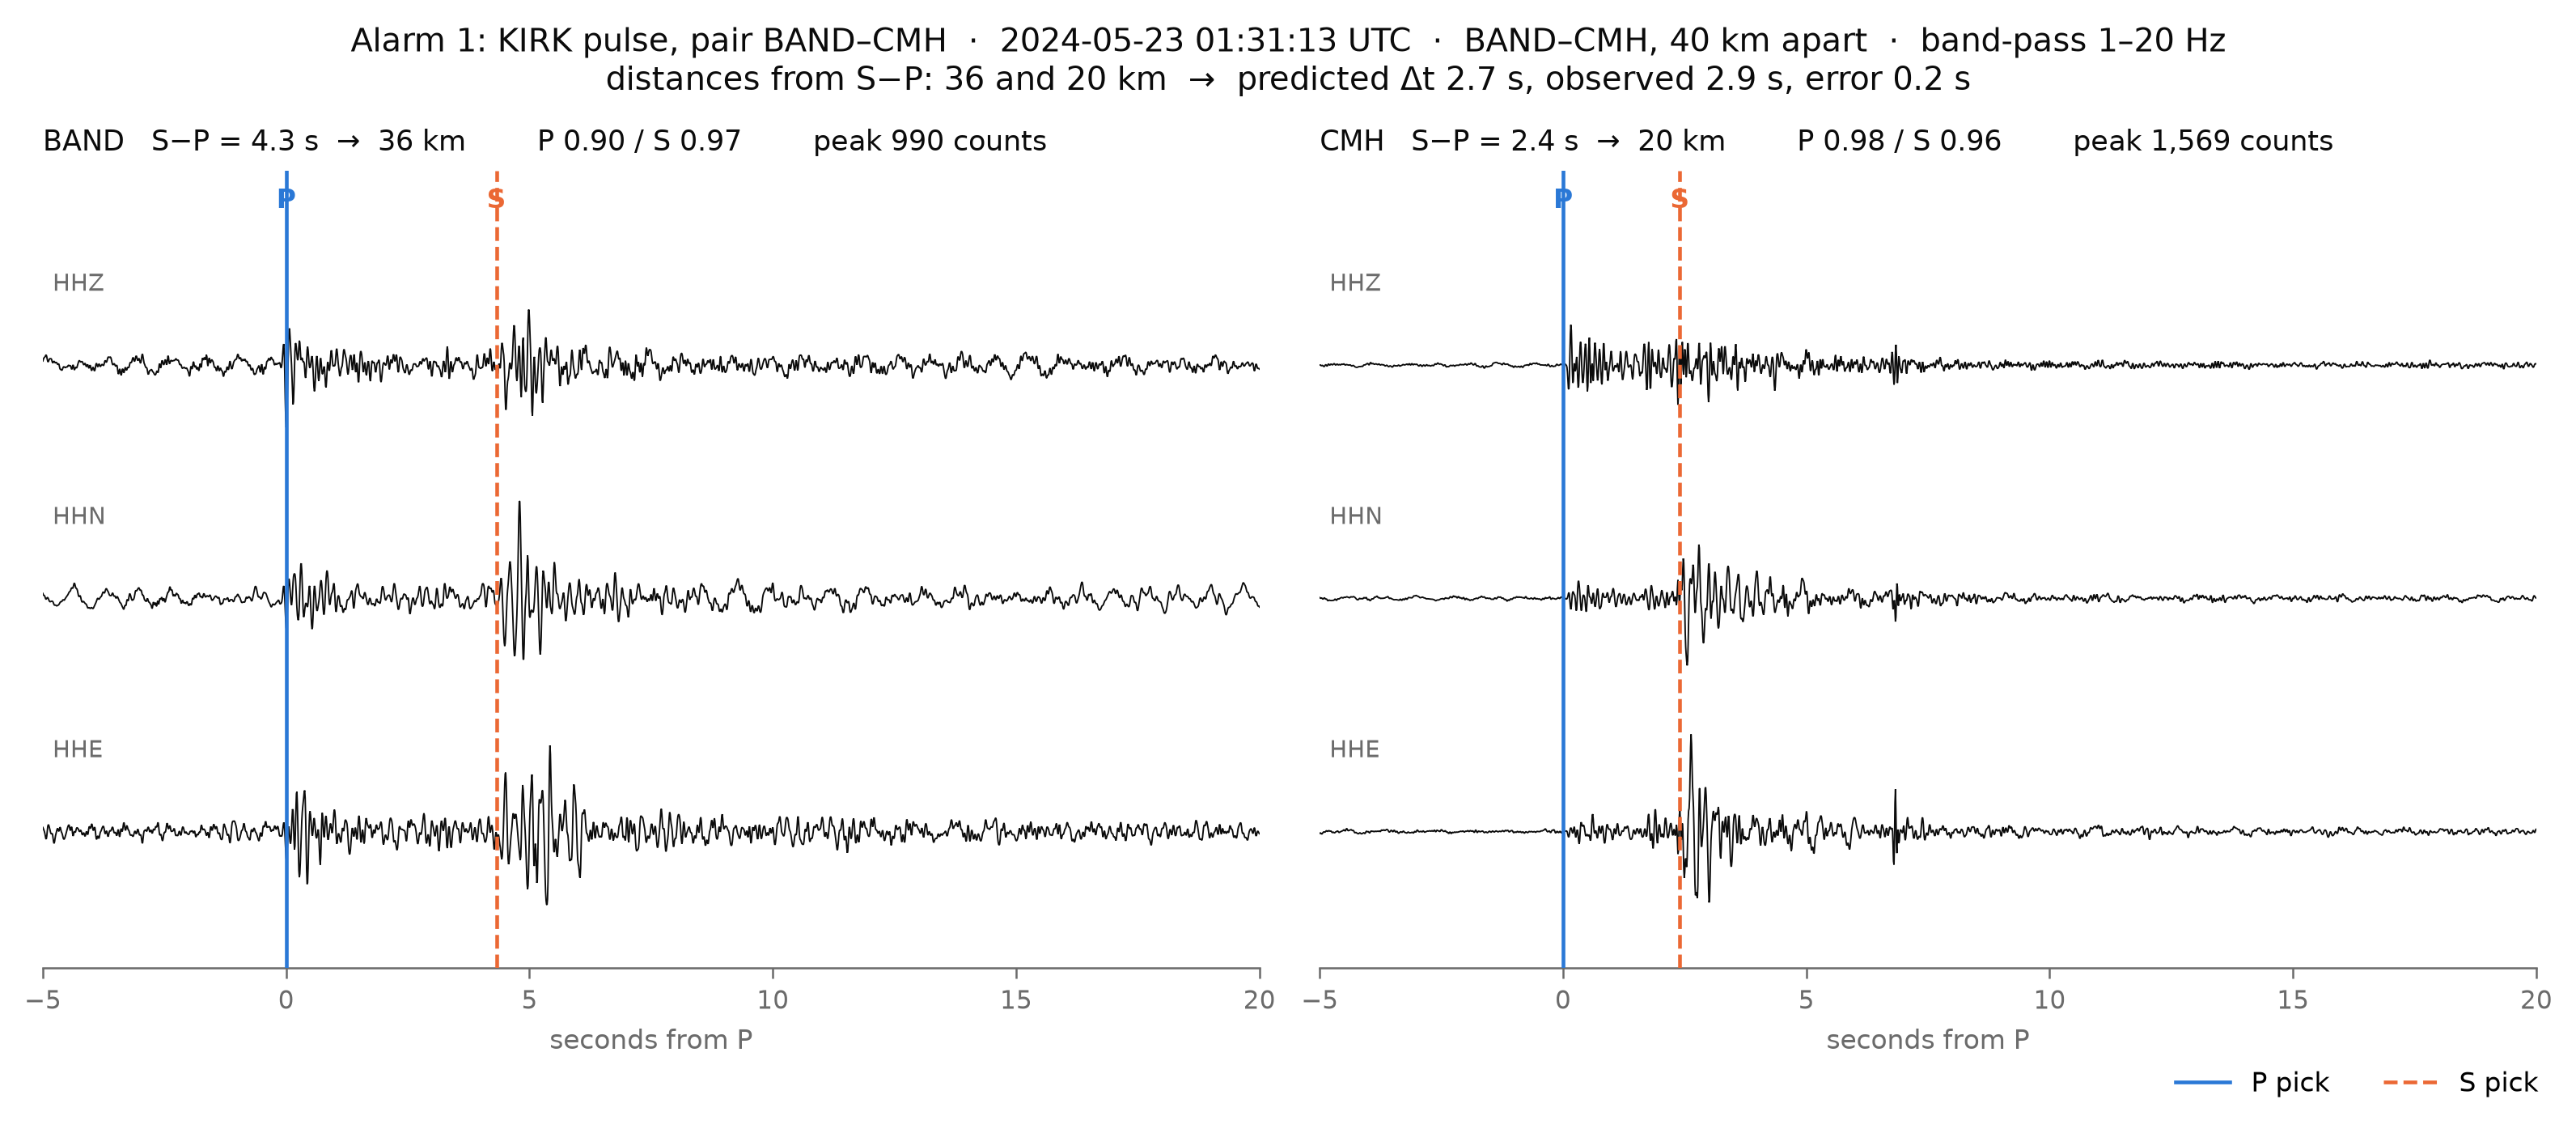
\includegraphics[width=\textwidth]{figures/supp/alarm01_BAND_CMH.png}
  \caption*{Alarm 1: KIRK pulse, pair BAND–CMH.}
\end{figure}
\begin{figure}[p]\centering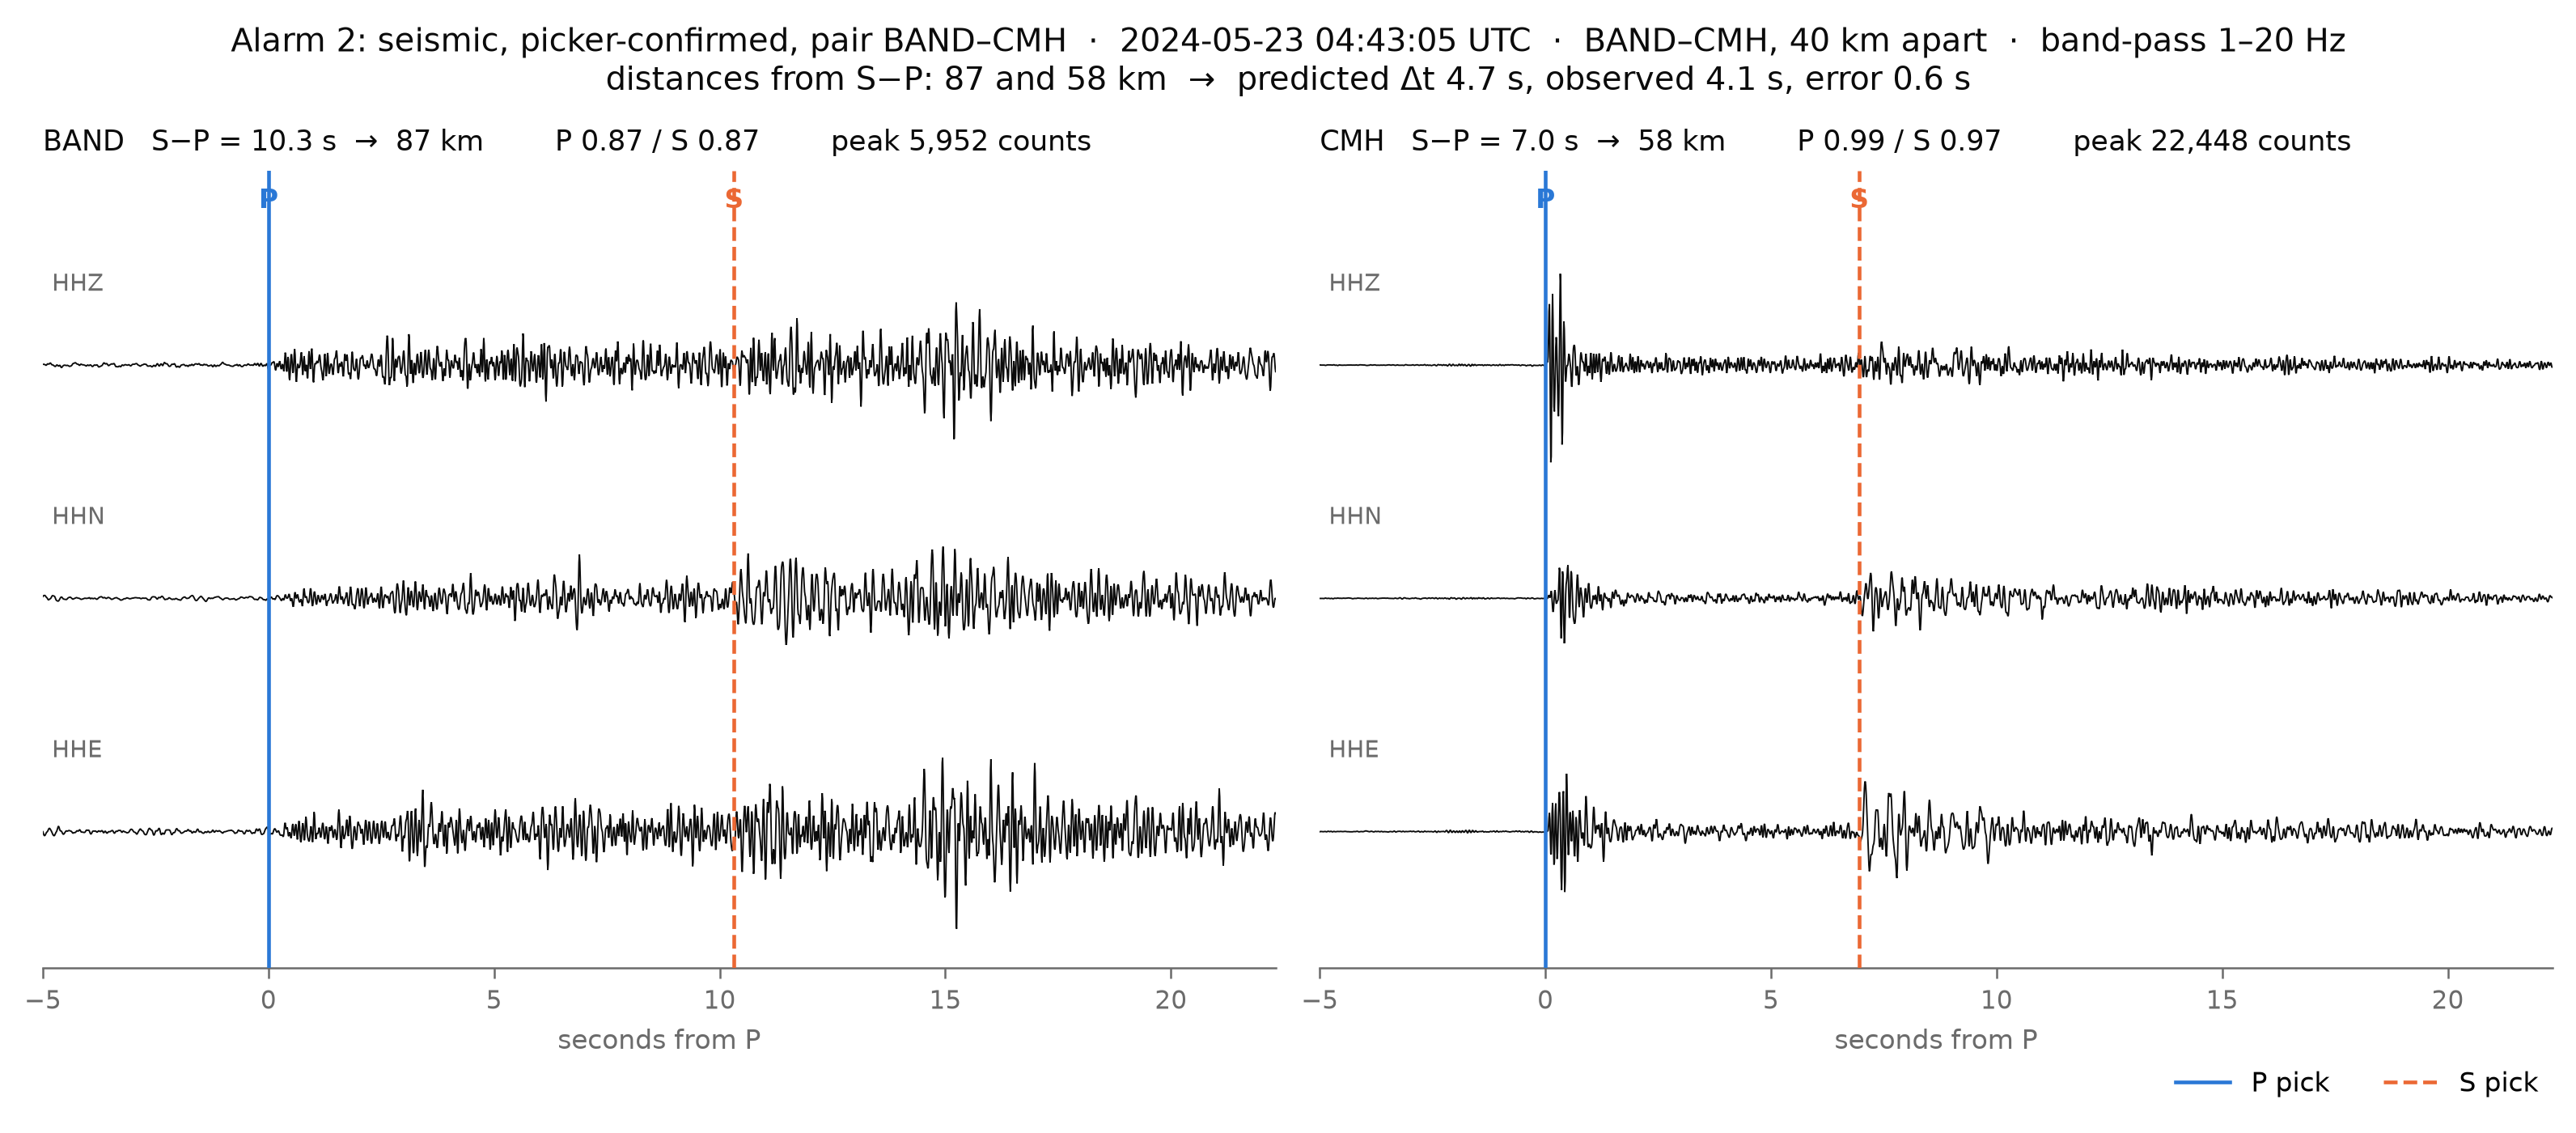
\includegraphics[width=\textwidth]{figures/supp/alarm02_BAND_CMH.png}
  \caption*{Alarm 2: seismic, picker-confirmed, pair BAND–CMH.}
\end{figure}
\begin{figure}[p]\centering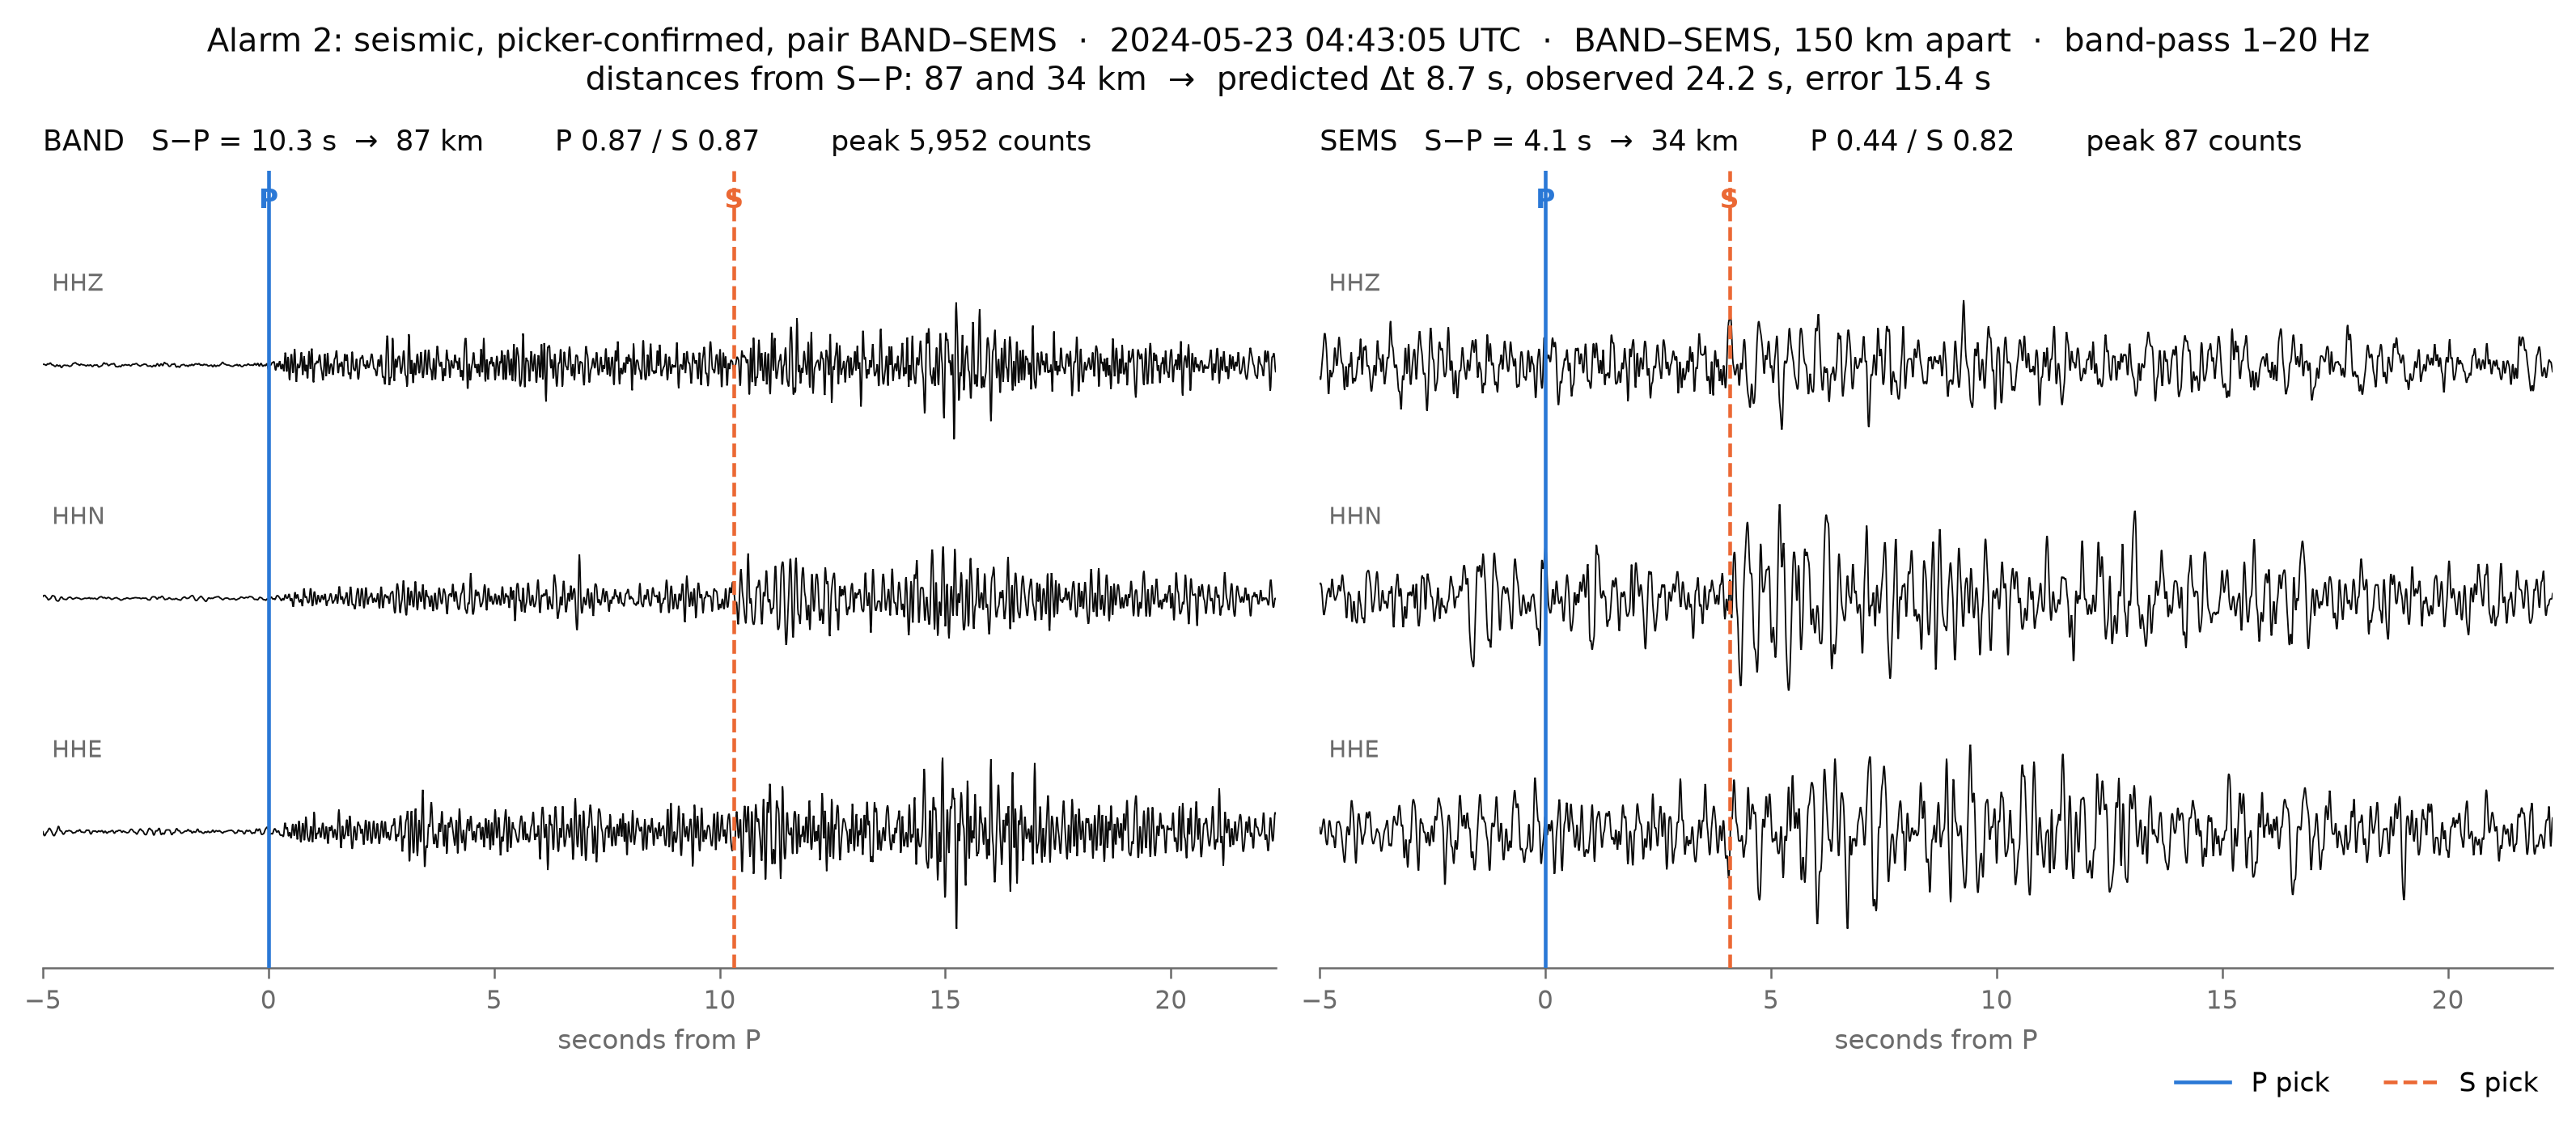
\includegraphics[width=\textwidth]{figures/supp/alarm02_BAND_SEMS.png}
  \caption*{Alarm 2: seismic, picker-confirmed, pair BAND–SEMS.}
\end{figure}
\begin{figure}[p]\centering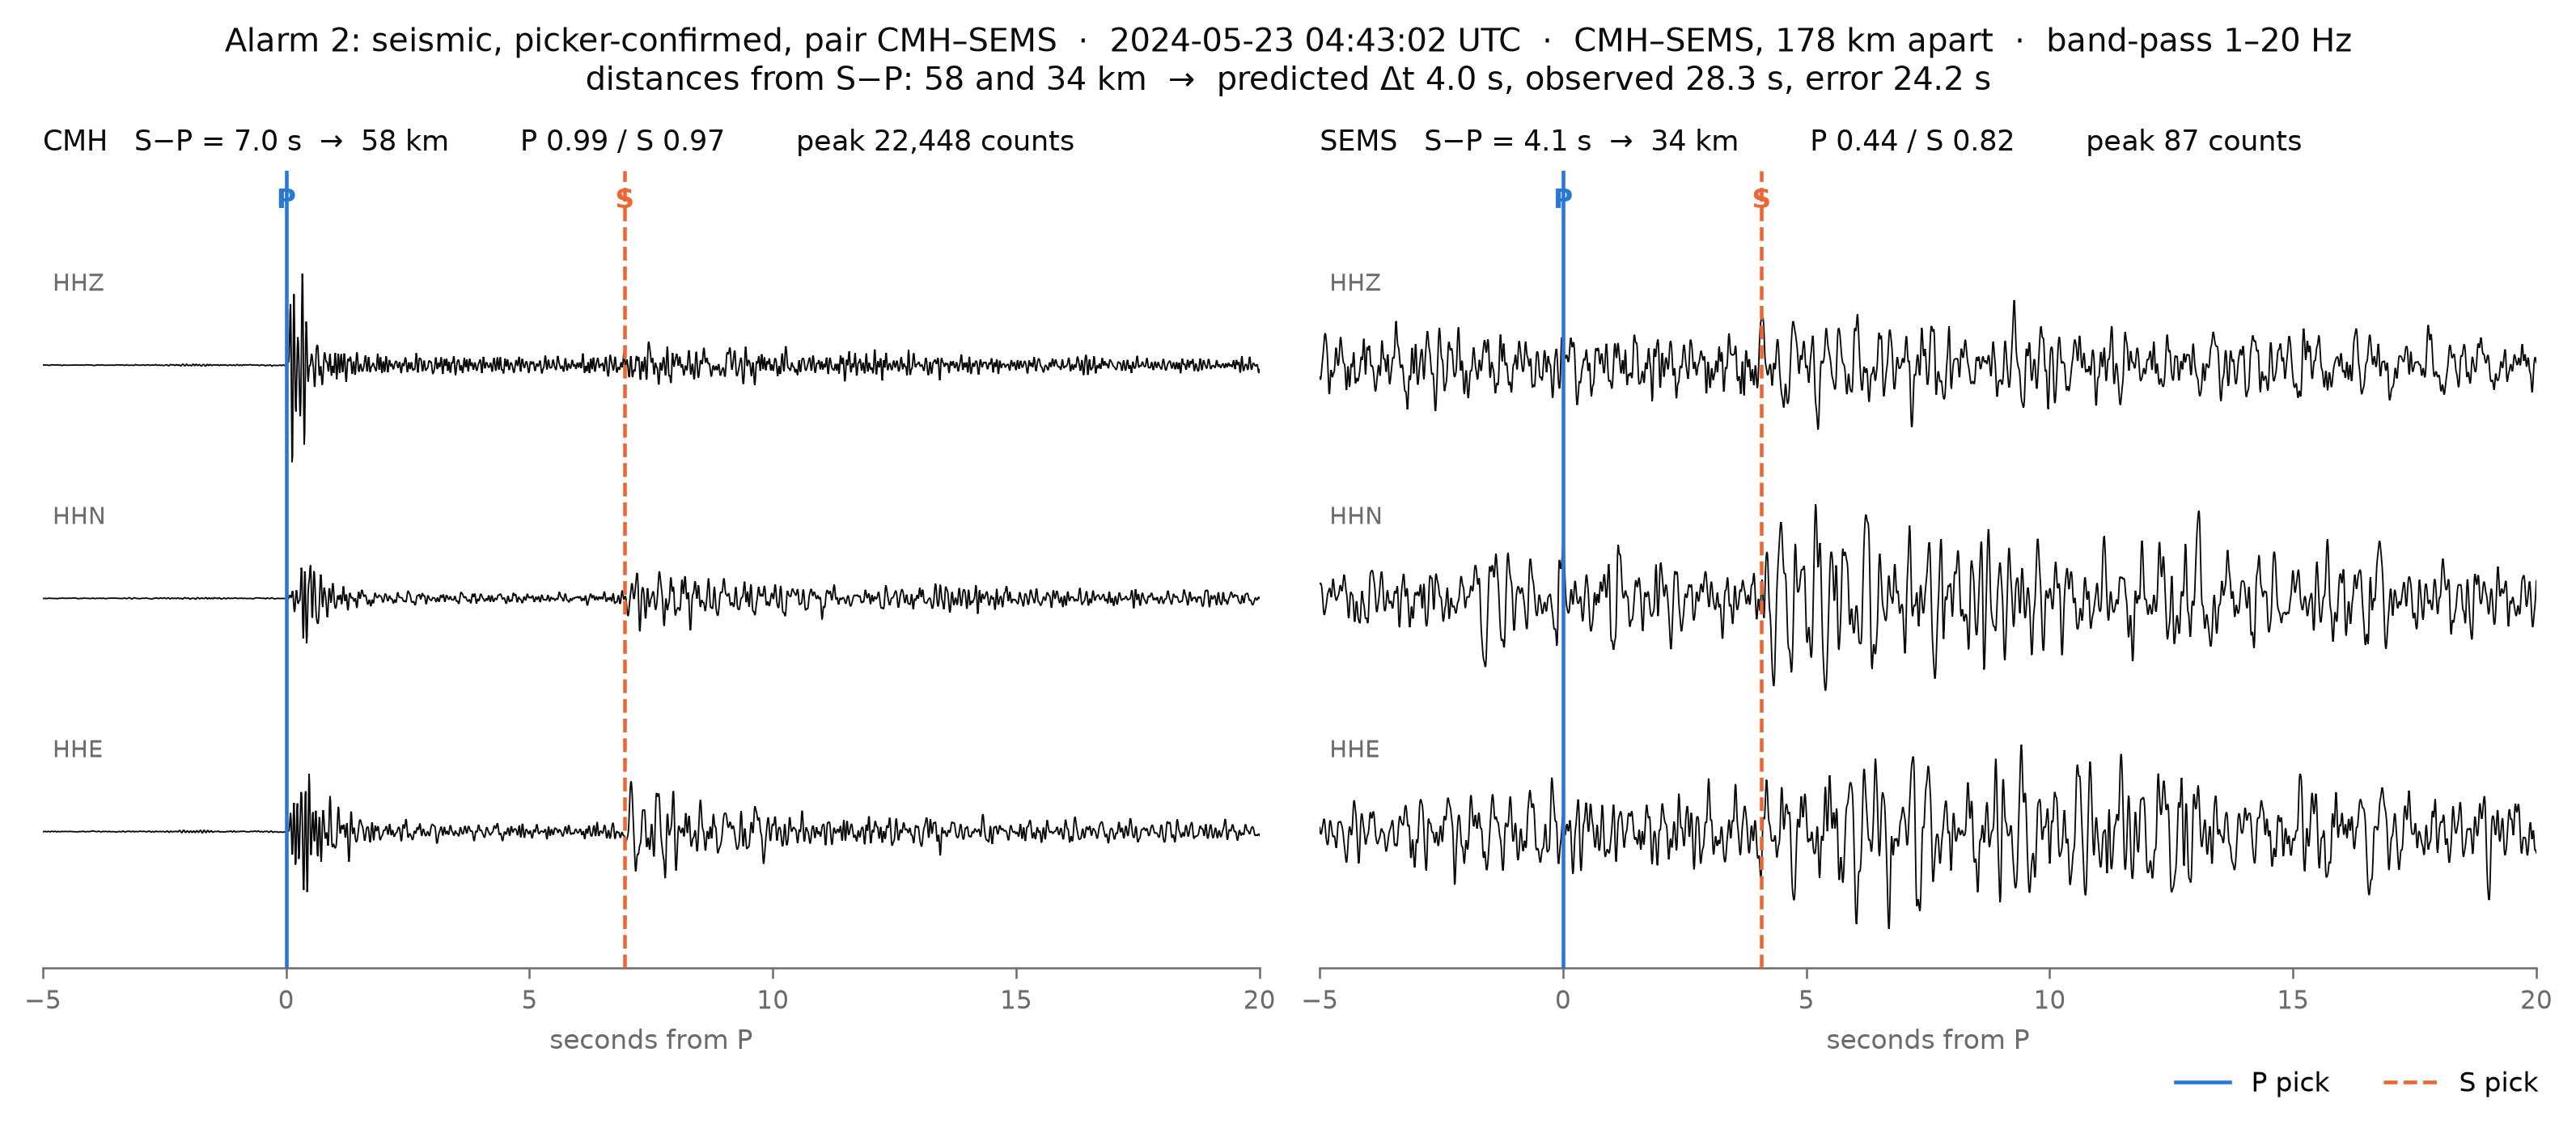
\includegraphics[width=\textwidth]{figures/supp/alarm02_CMH_SEMS.png}
  \caption*{Alarm 2: seismic, picker-confirmed, pair CMH–SEMS.}
\end{figure}
\begin{figure}[p]\centering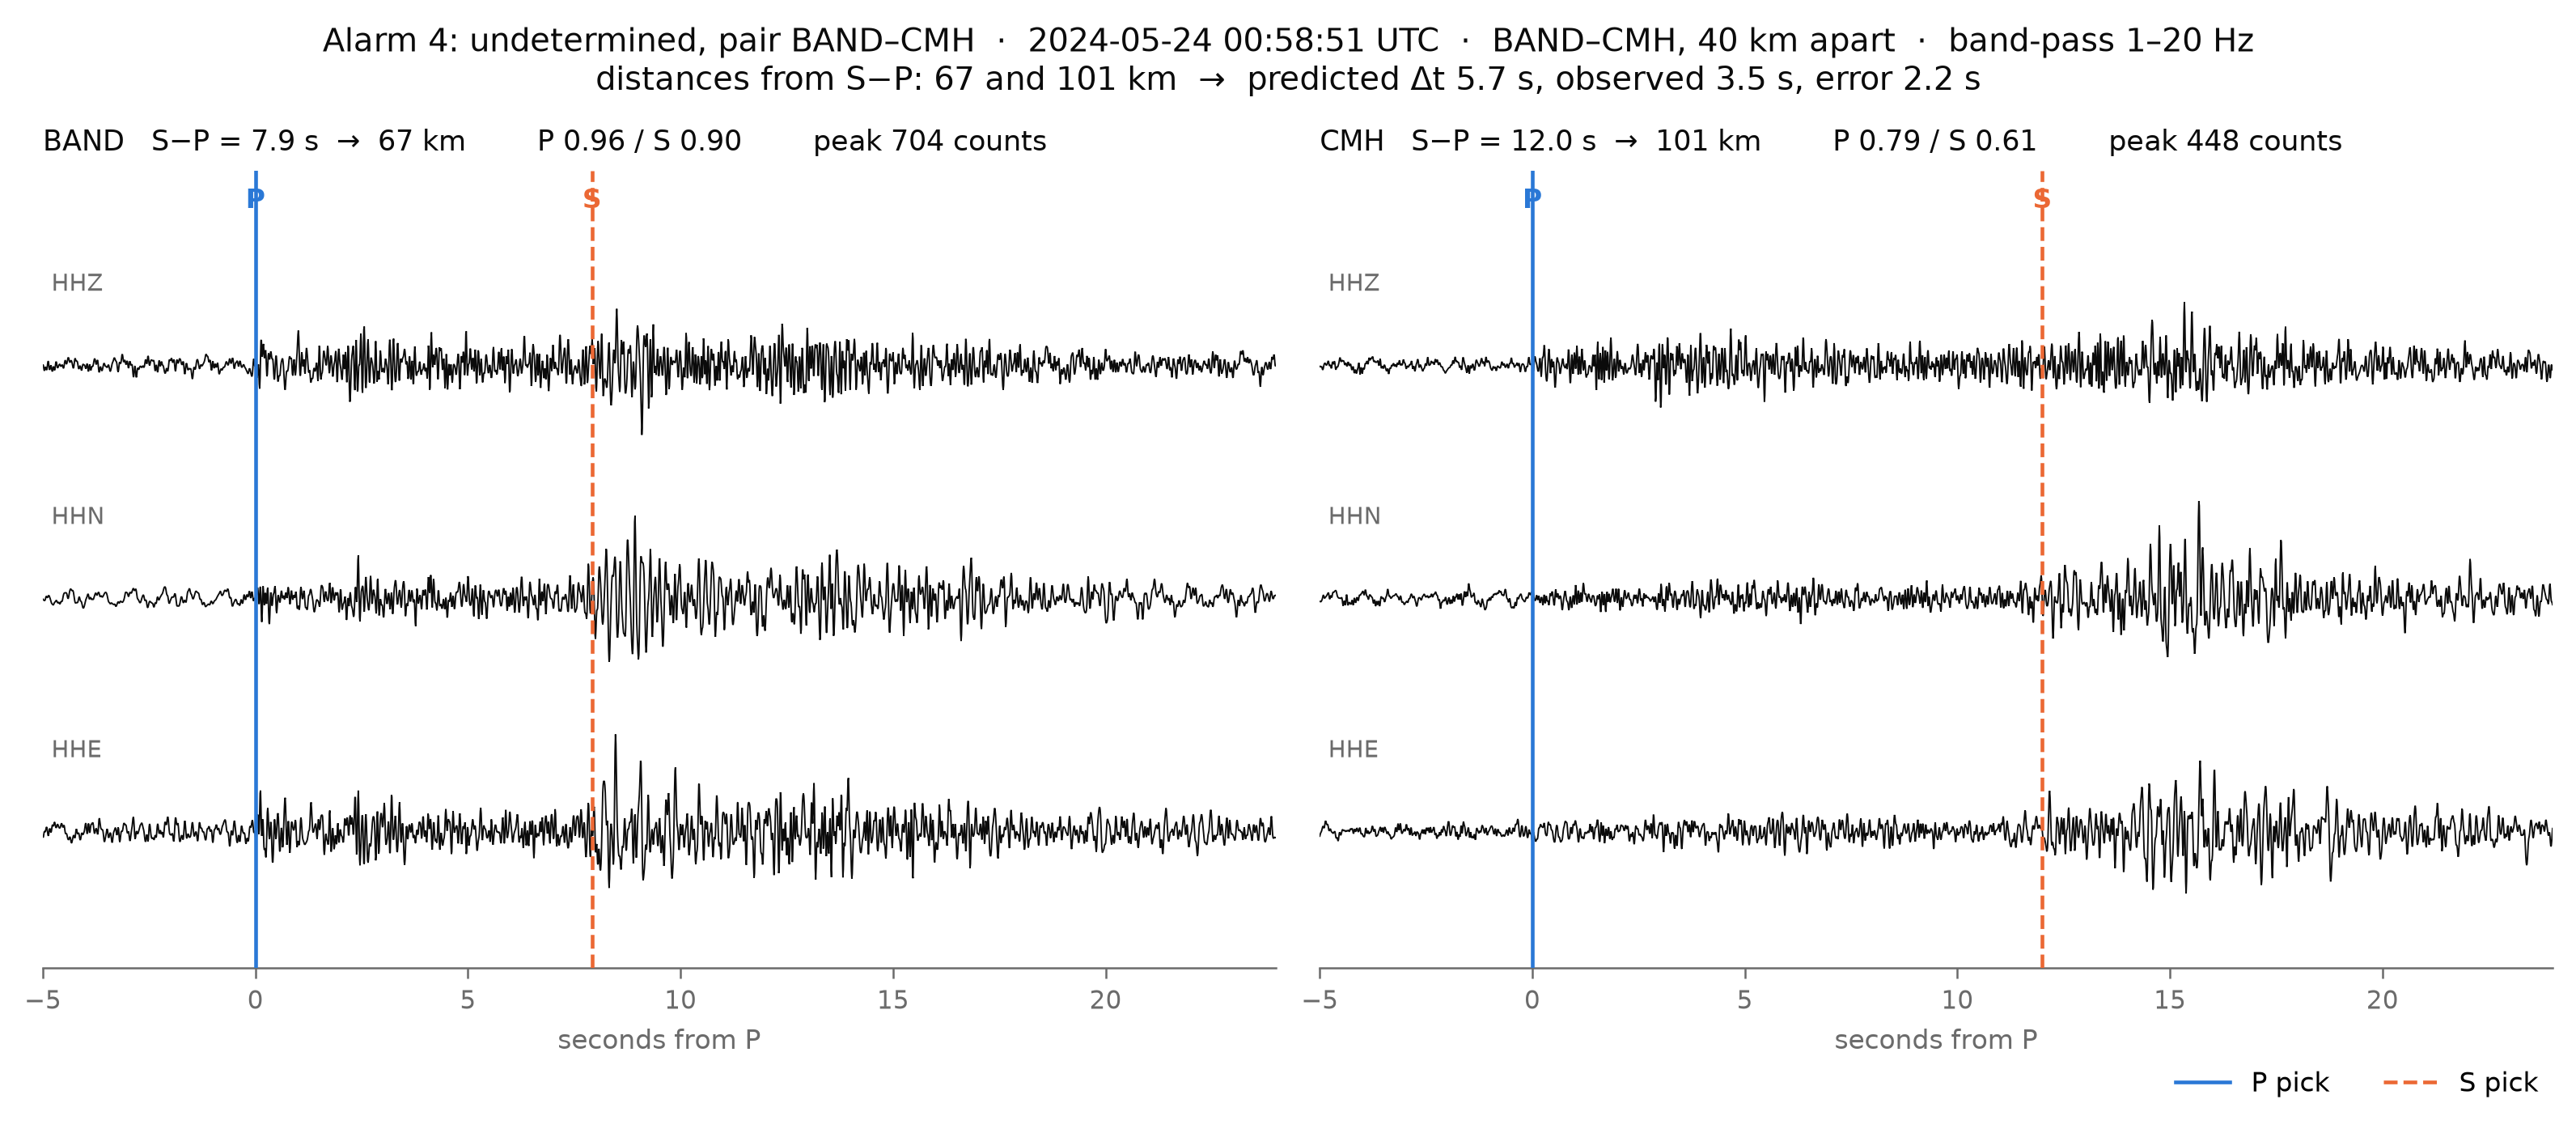
\includegraphics[width=\textwidth]{figures/supp/alarm04_BAND_CMH.png}
  \caption*{Alarm 4: undetermined, pair BAND–CMH.}
\end{figure}
\begin{figure}[p]\centering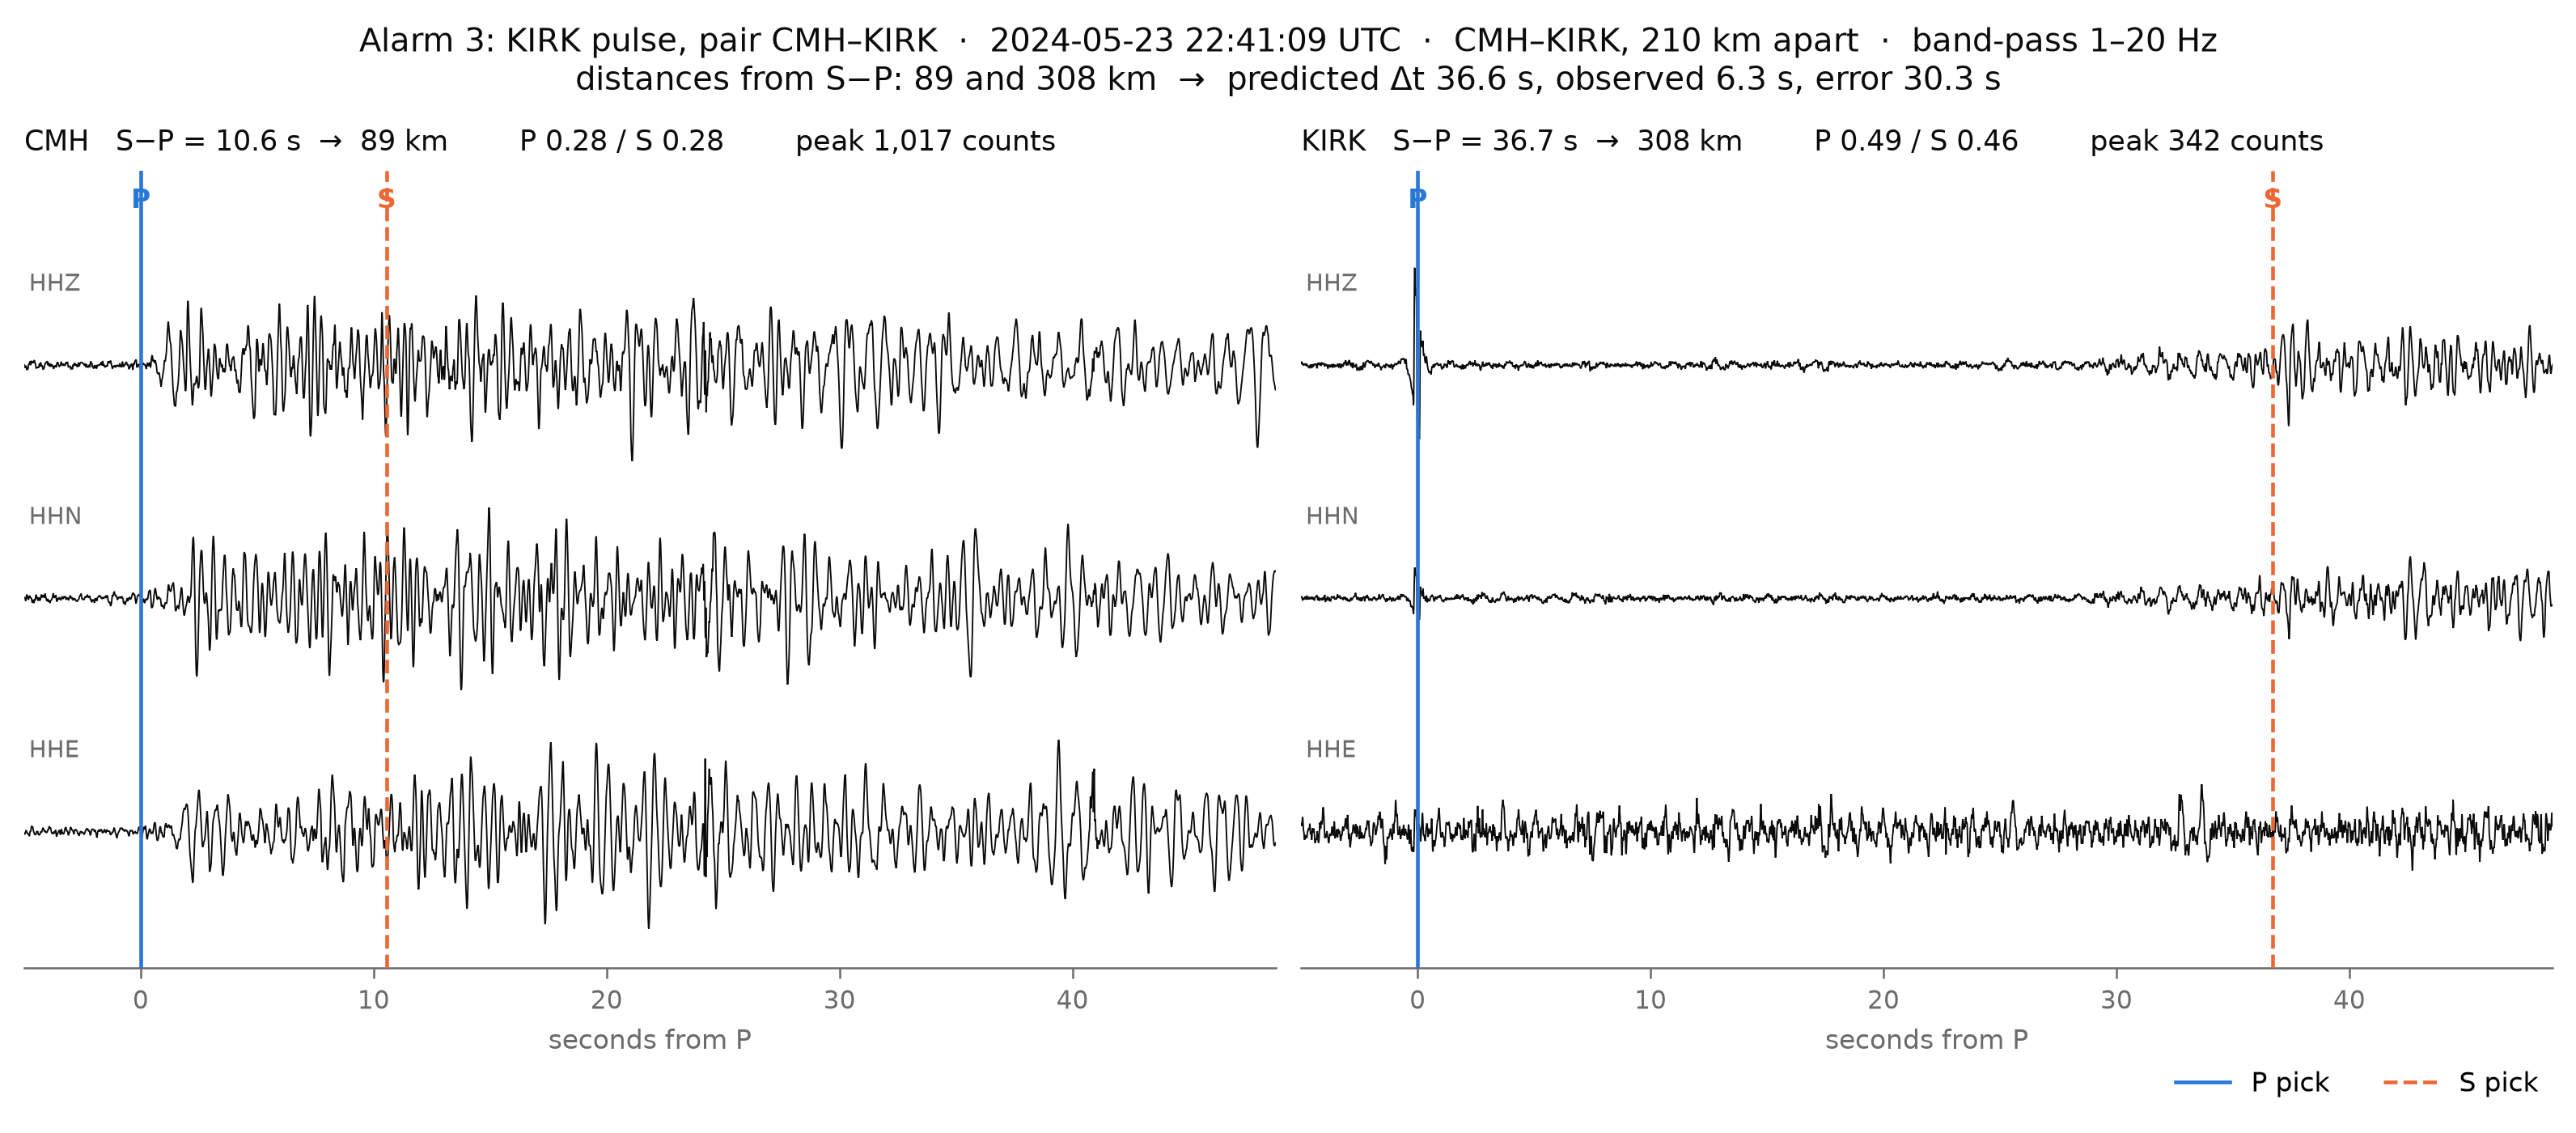
\includegraphics[width=\textwidth]{figures/supp/alarm03_CMH_KIRK.png}
  \caption*{Alarm 3: KIRK pulse, pair CMH–KIRK.}
\end{figure}
\begin{figure}[p]\centering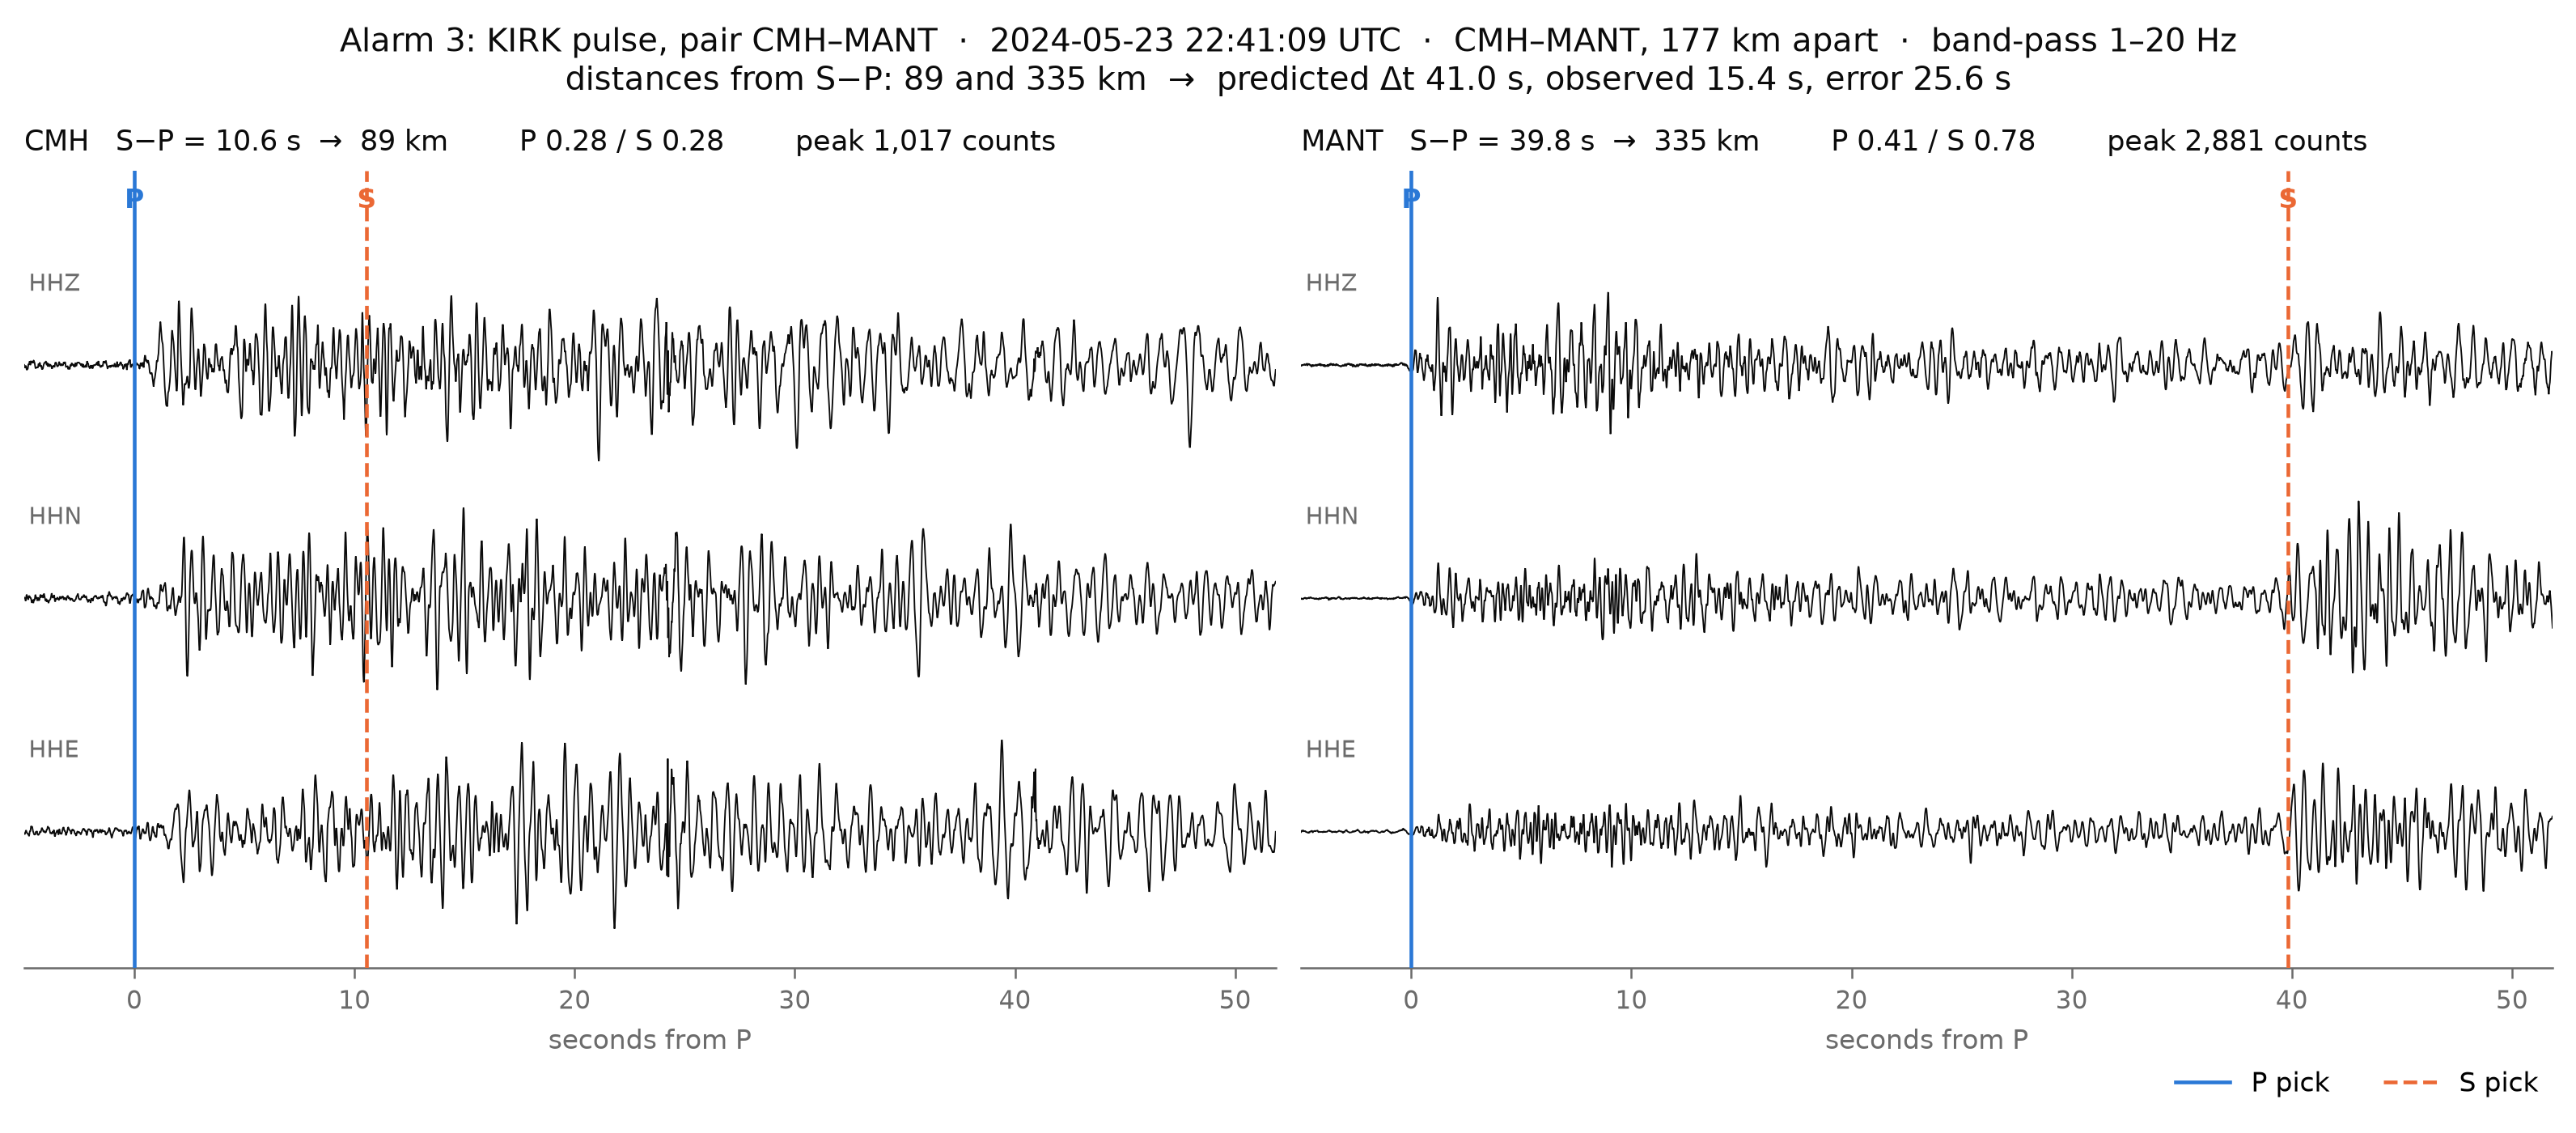
\includegraphics[width=\textwidth]{figures/supp/alarm03_CMH_MANT.png}
  \caption*{Alarm 3: KIRK pulse, pair CMH–MANT.}
\end{figure}
\begin{figure}[p]\centering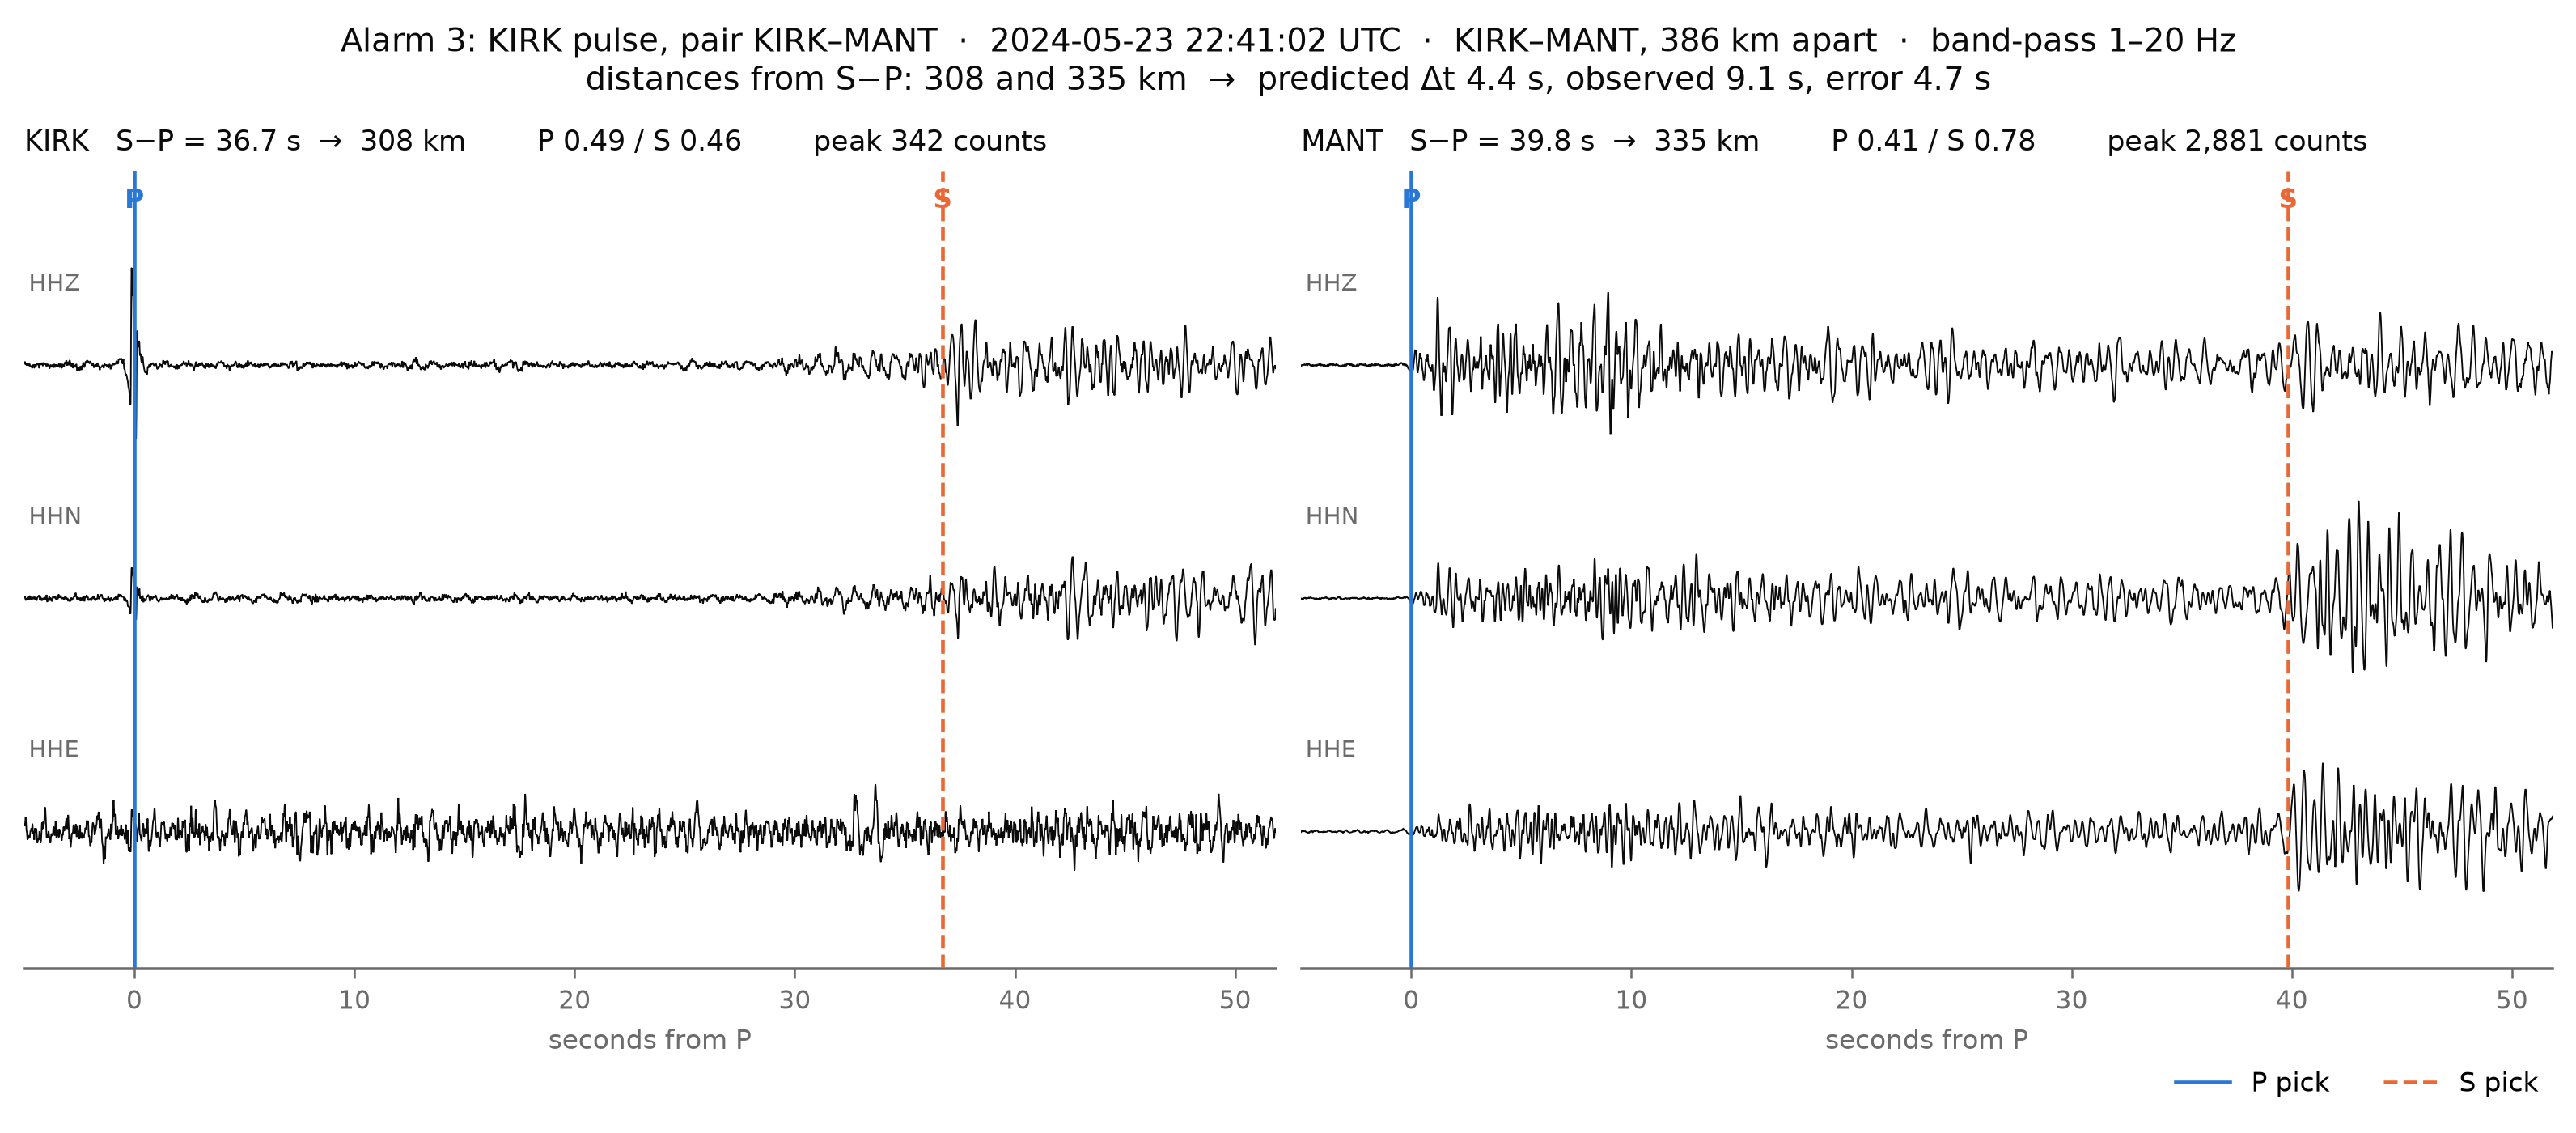
\includegraphics[width=\textwidth]{figures/supp/alarm03_KIRK_MANT.png}
  \caption*{Alarm 3: KIRK pulse, pair KIRK–MANT.}
\end{figure}
\begin{figure}[p]\centering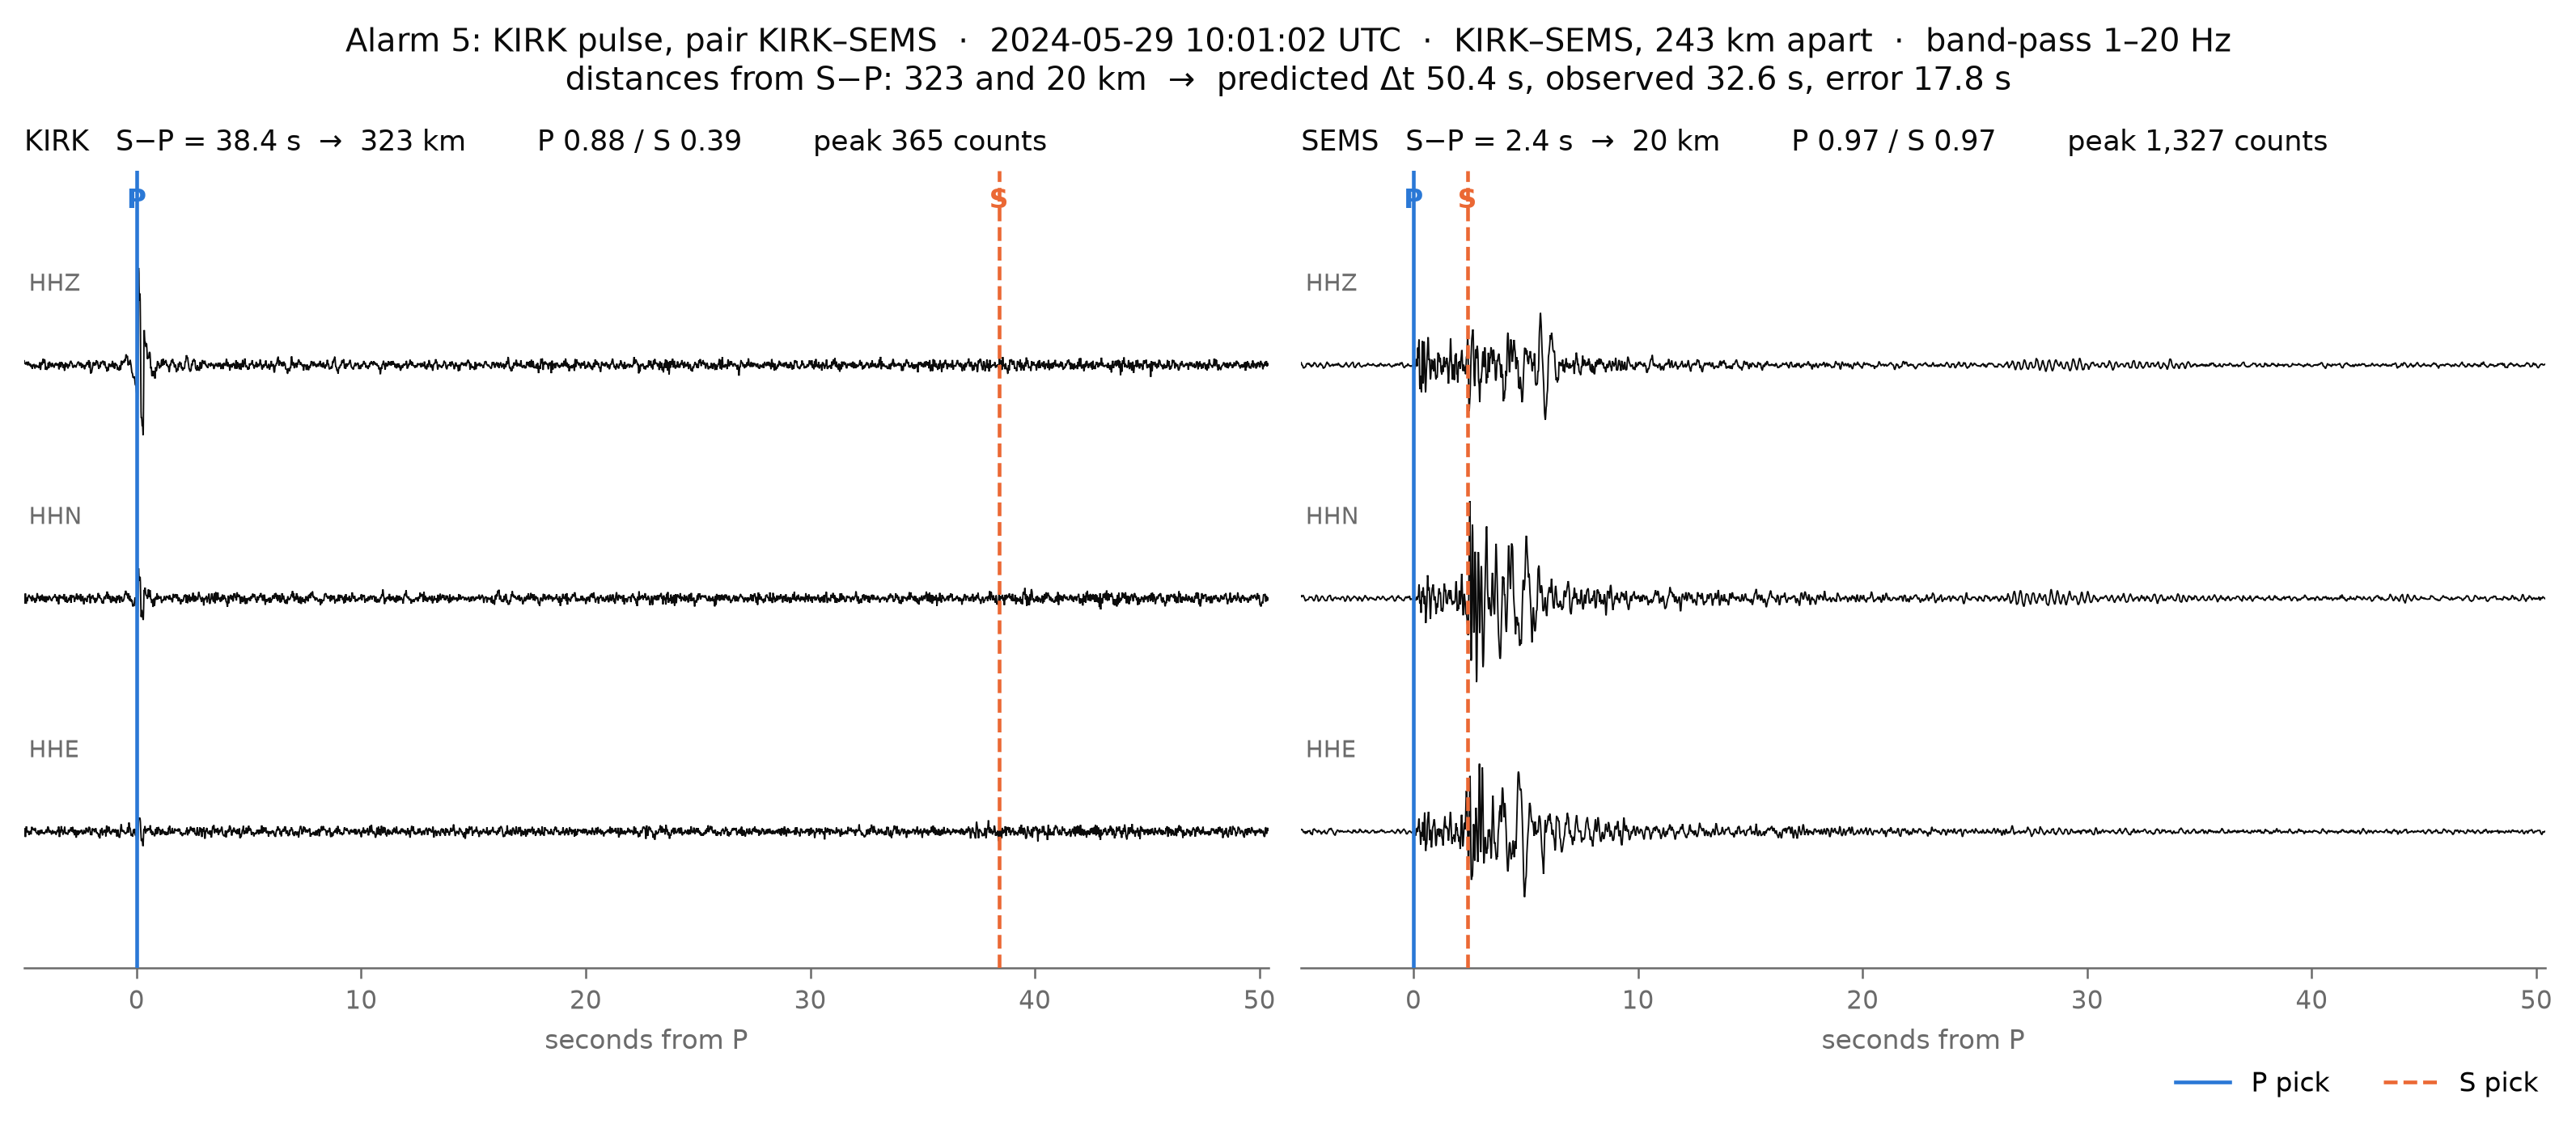
\includegraphics[width=\textwidth]{figures/supp/alarm05_KIRK_SEMS.png}
  \caption*{Alarm 5: KIRK pulse, pair KIRK–SEMS.}
\end{figure}
\begin{figure}[p]\centering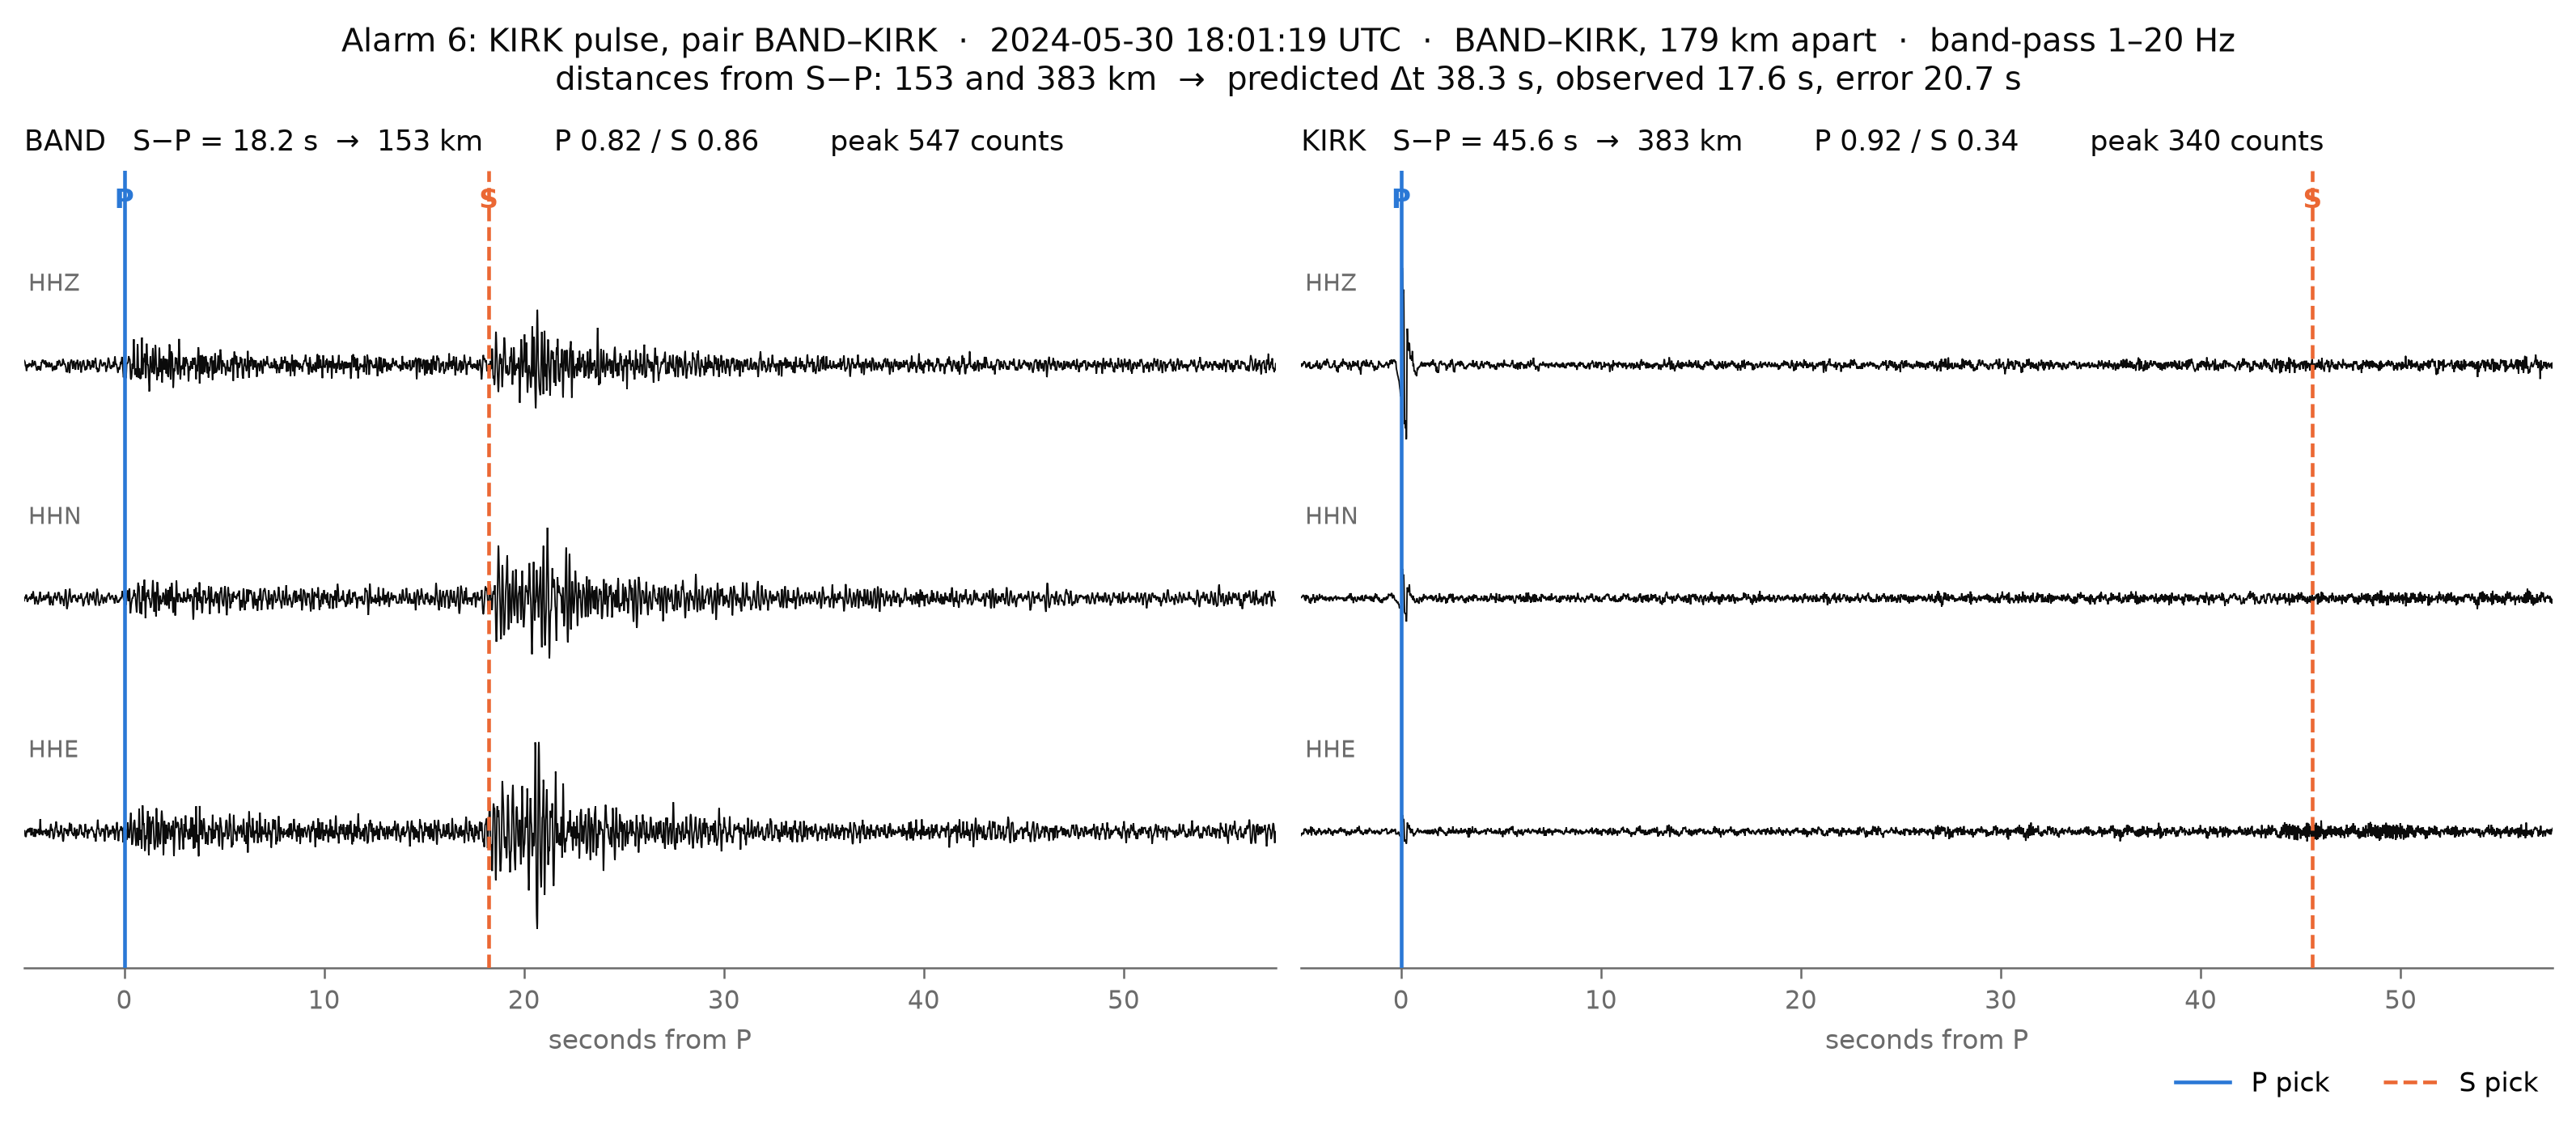
\includegraphics[width=\textwidth]{figures/supp/alarm06_BAND_KIRK.png}
  \caption*{Alarm 6: KIRK pulse, pair BAND–KIRK.}
\end{figure}
\begin{figure}[p]\centering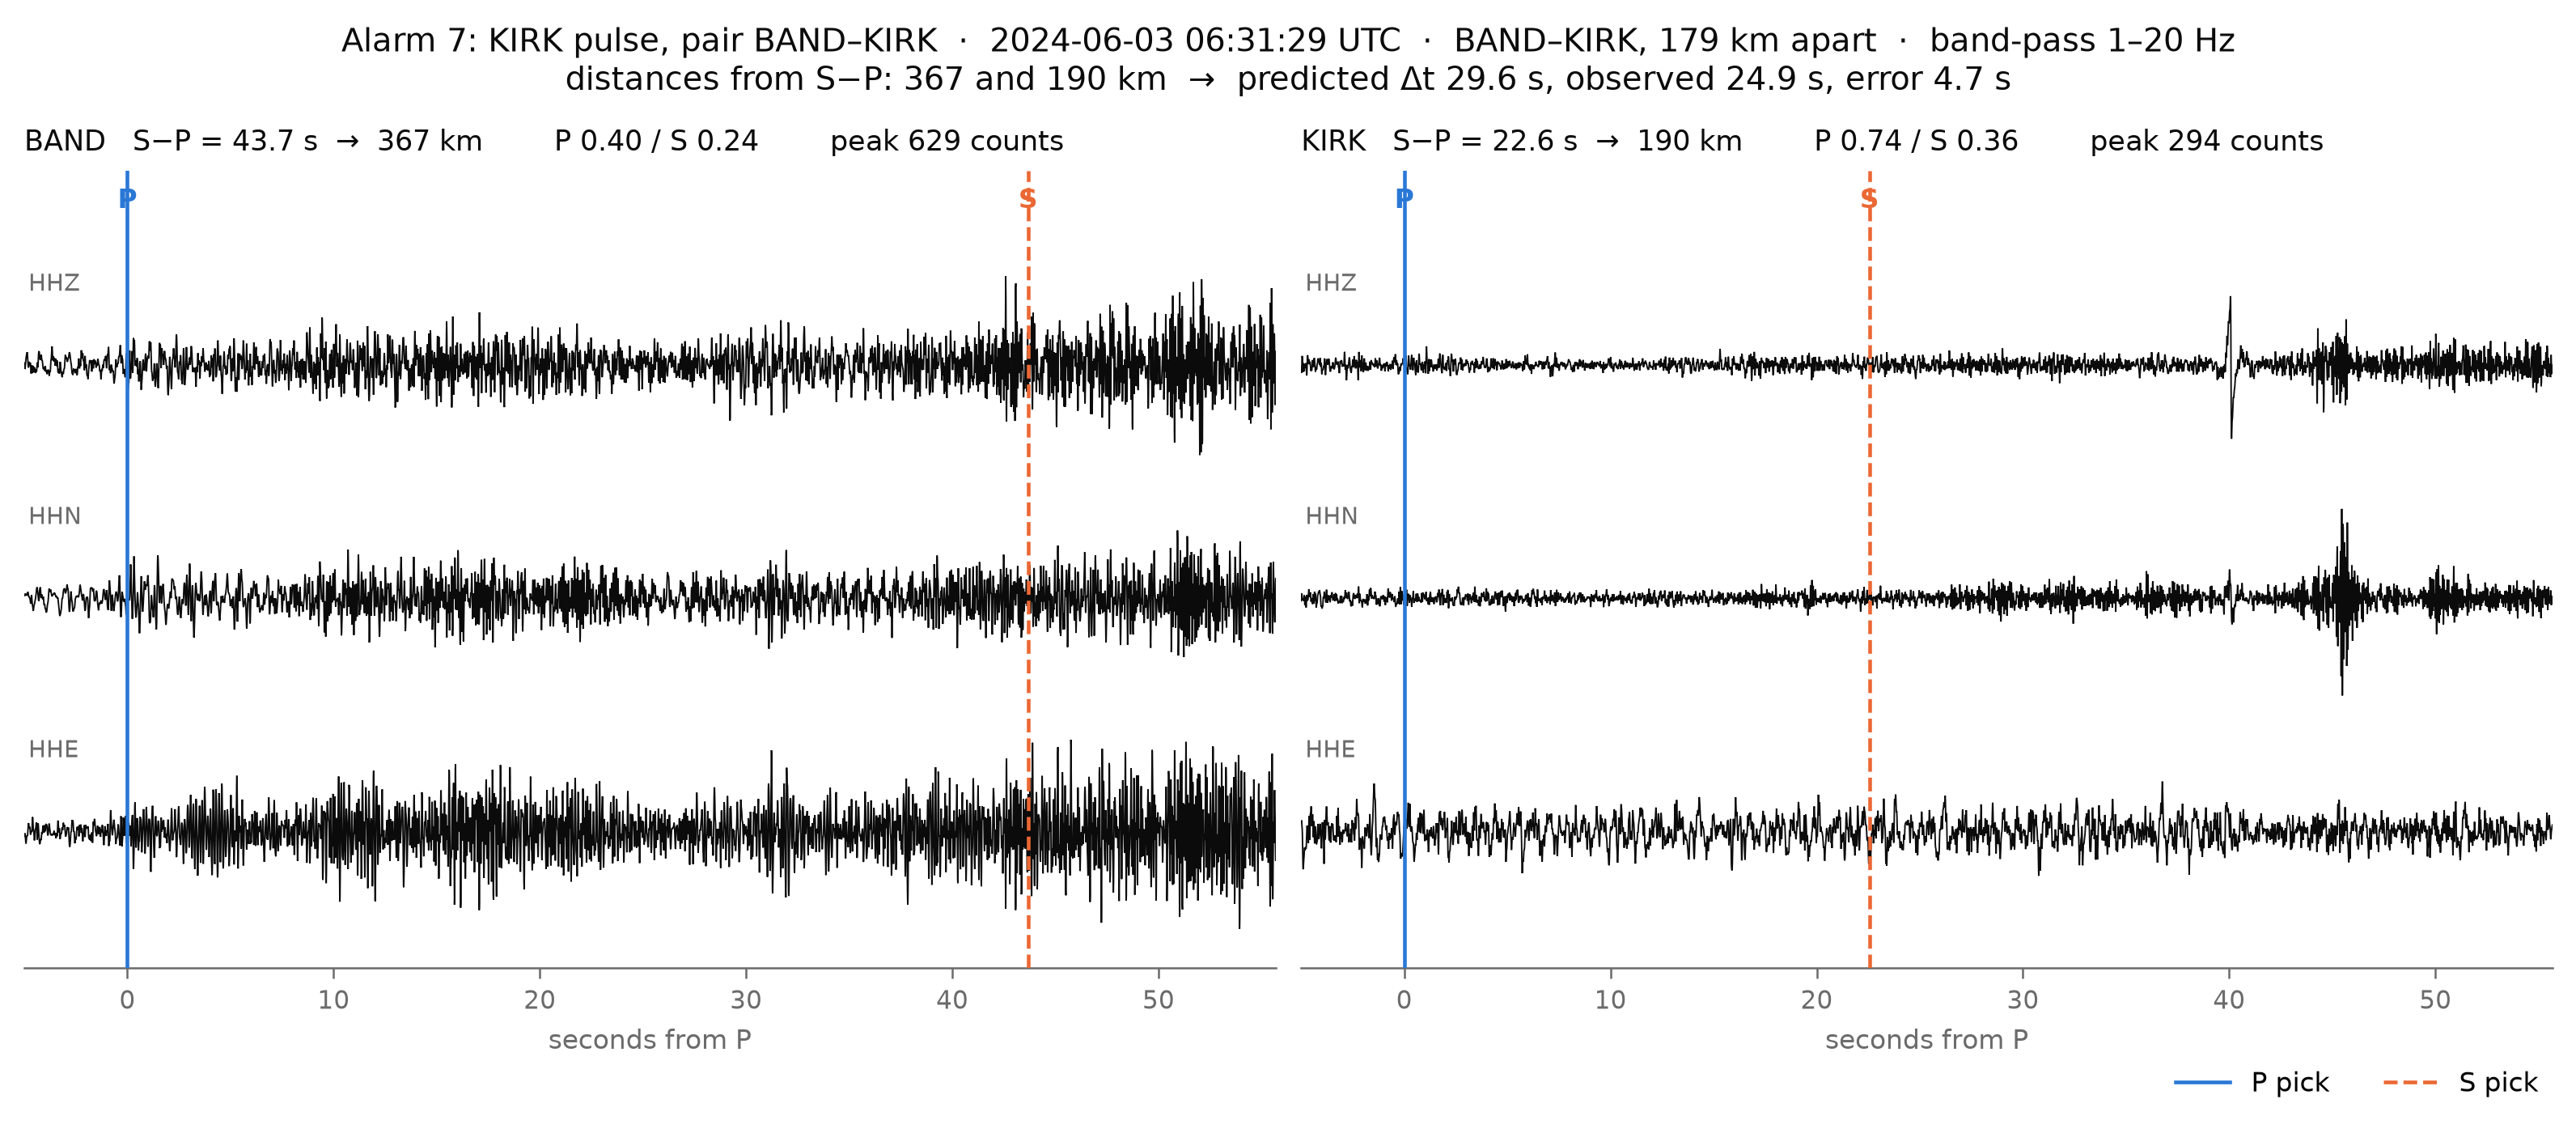
\includegraphics[width=\textwidth]{figures/supp/alarm07_BAND_KIRK.png}
  \caption*{Alarm 7: KIRK pulse, pair BAND–KIRK.}
\end{figure}
\begin{figure}[p]\centering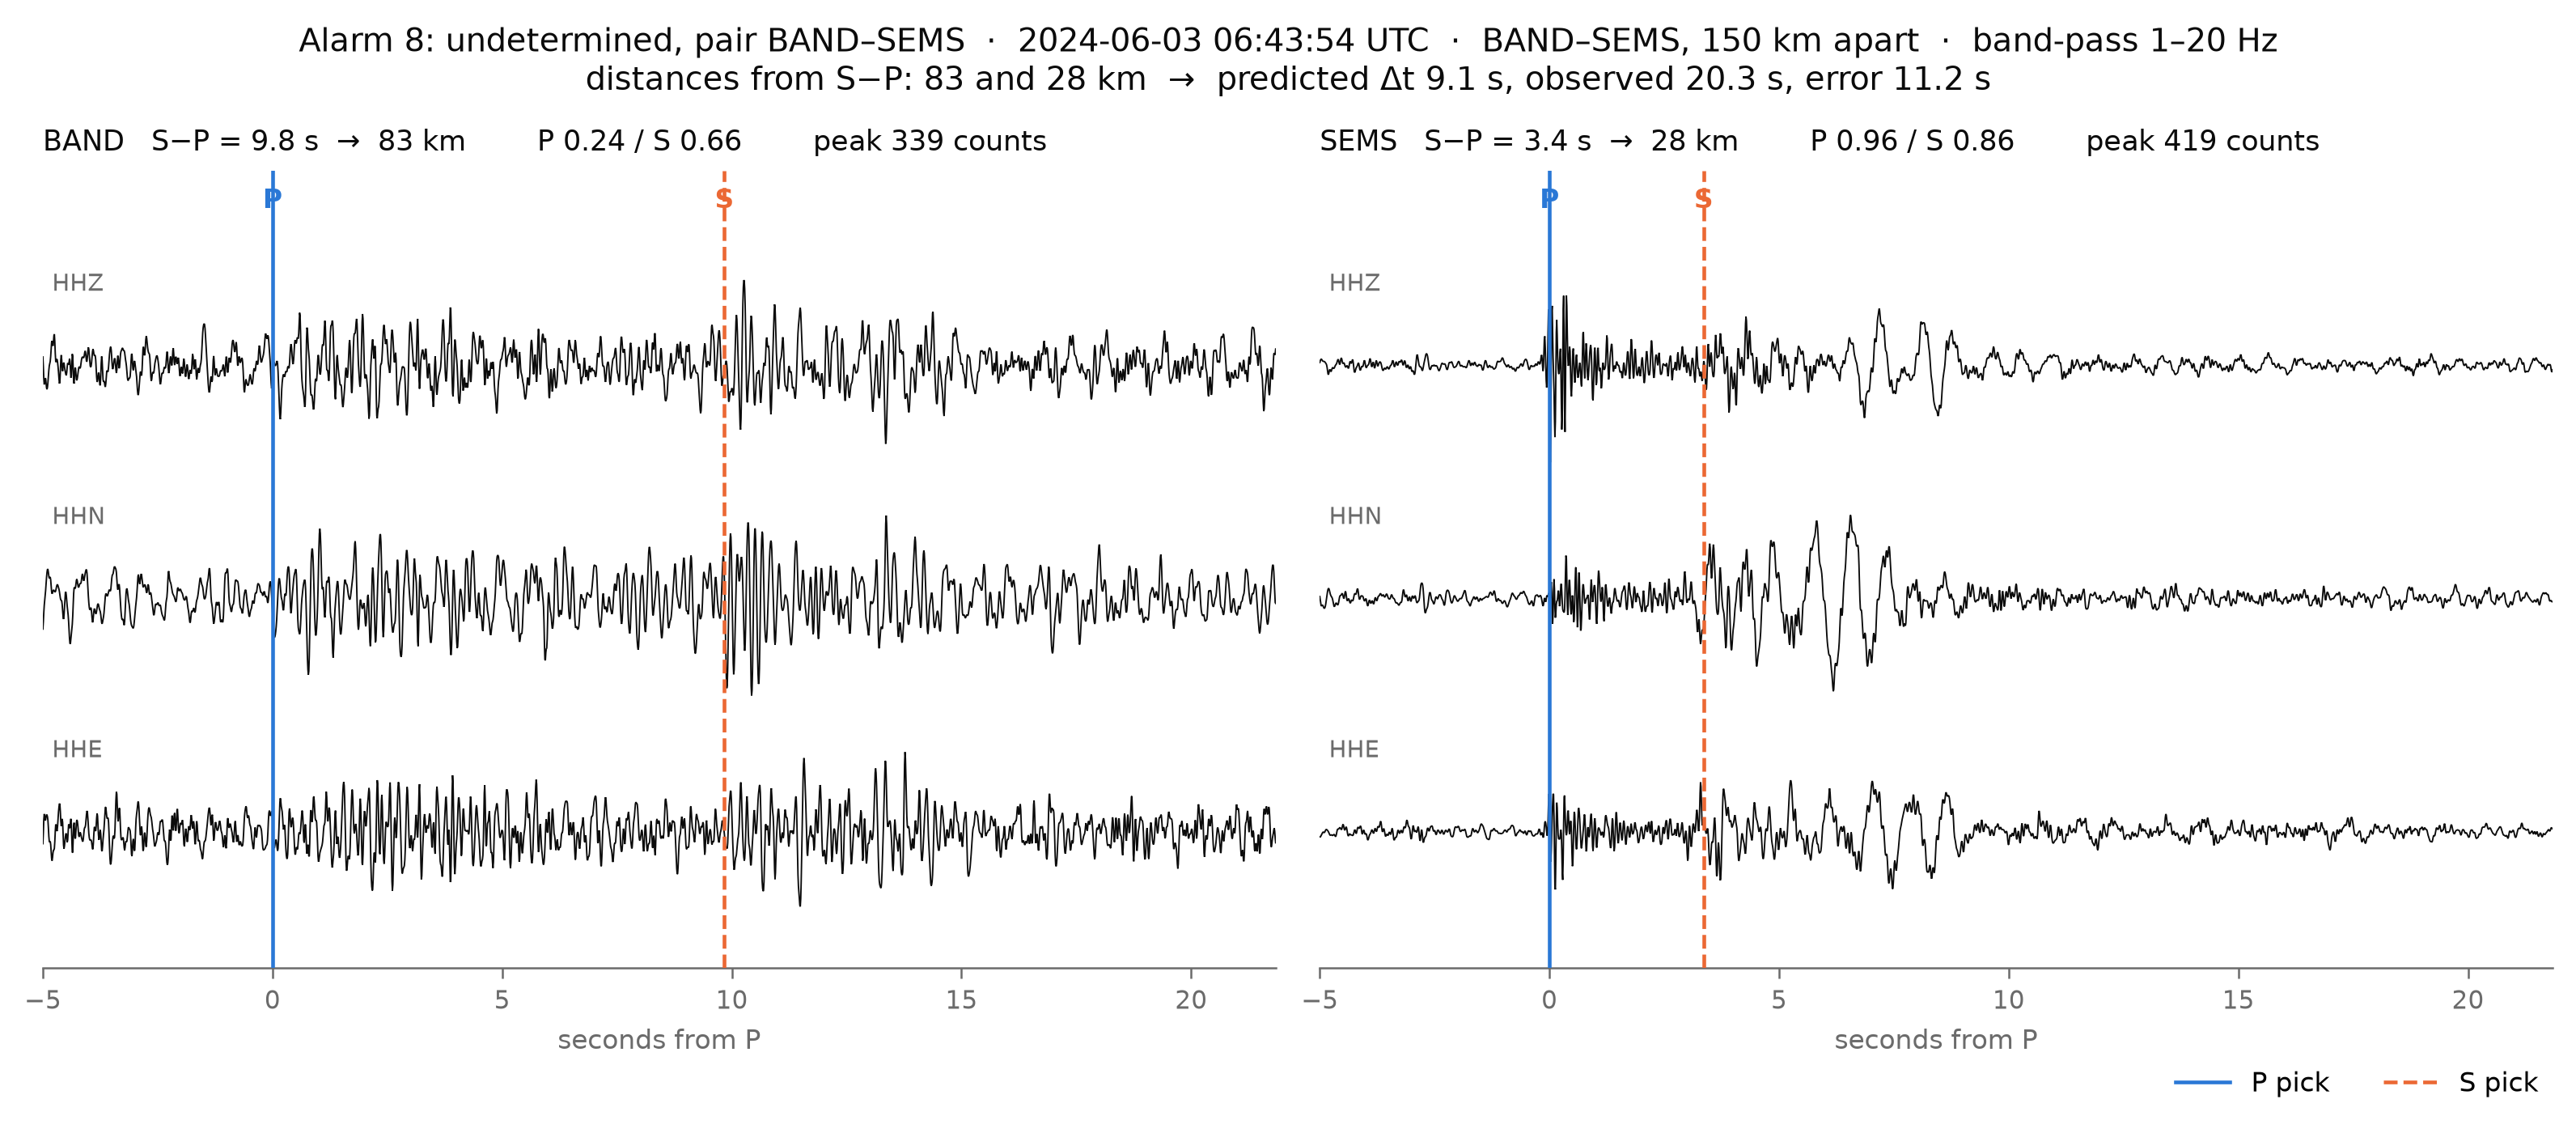
\includegraphics[width=\textwidth]{figures/supp/alarm08_BAND_SEMS.png}
  \caption*{Alarm 8: undetermined, pair BAND–SEMS.}
\end{figure}
\begin{figure}[p]\centering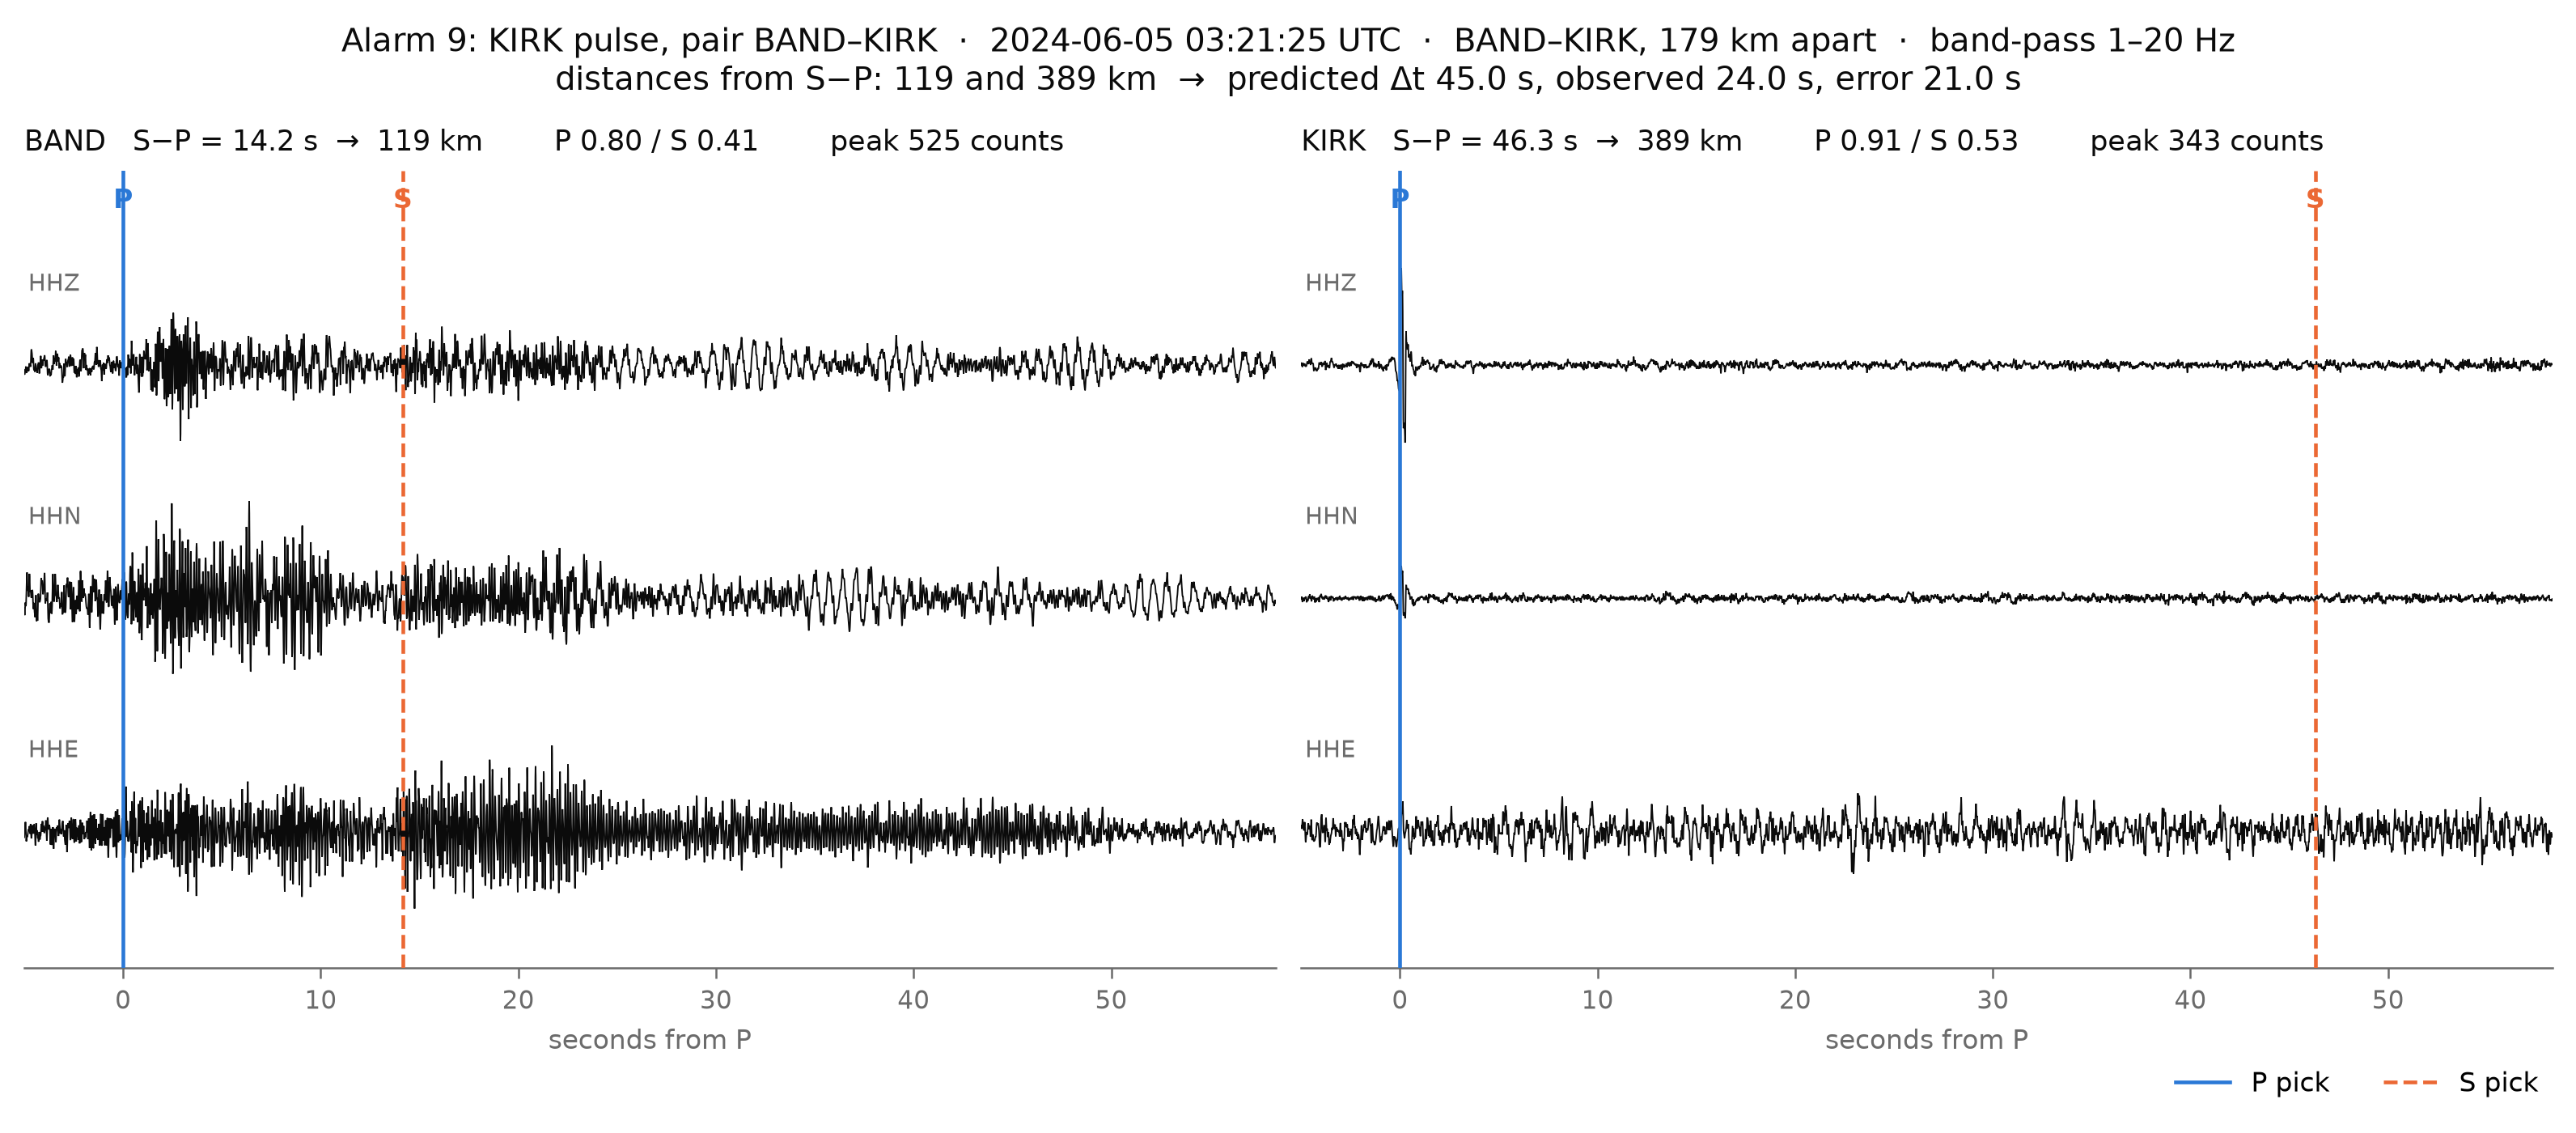
\includegraphics[width=\textwidth]{figures/supp/alarm09_BAND_KIRK.png}
  \caption*{Alarm 9: KIRK pulse, pair BAND–KIRK.}
\end{figure}
\begin{figure}[p]\centering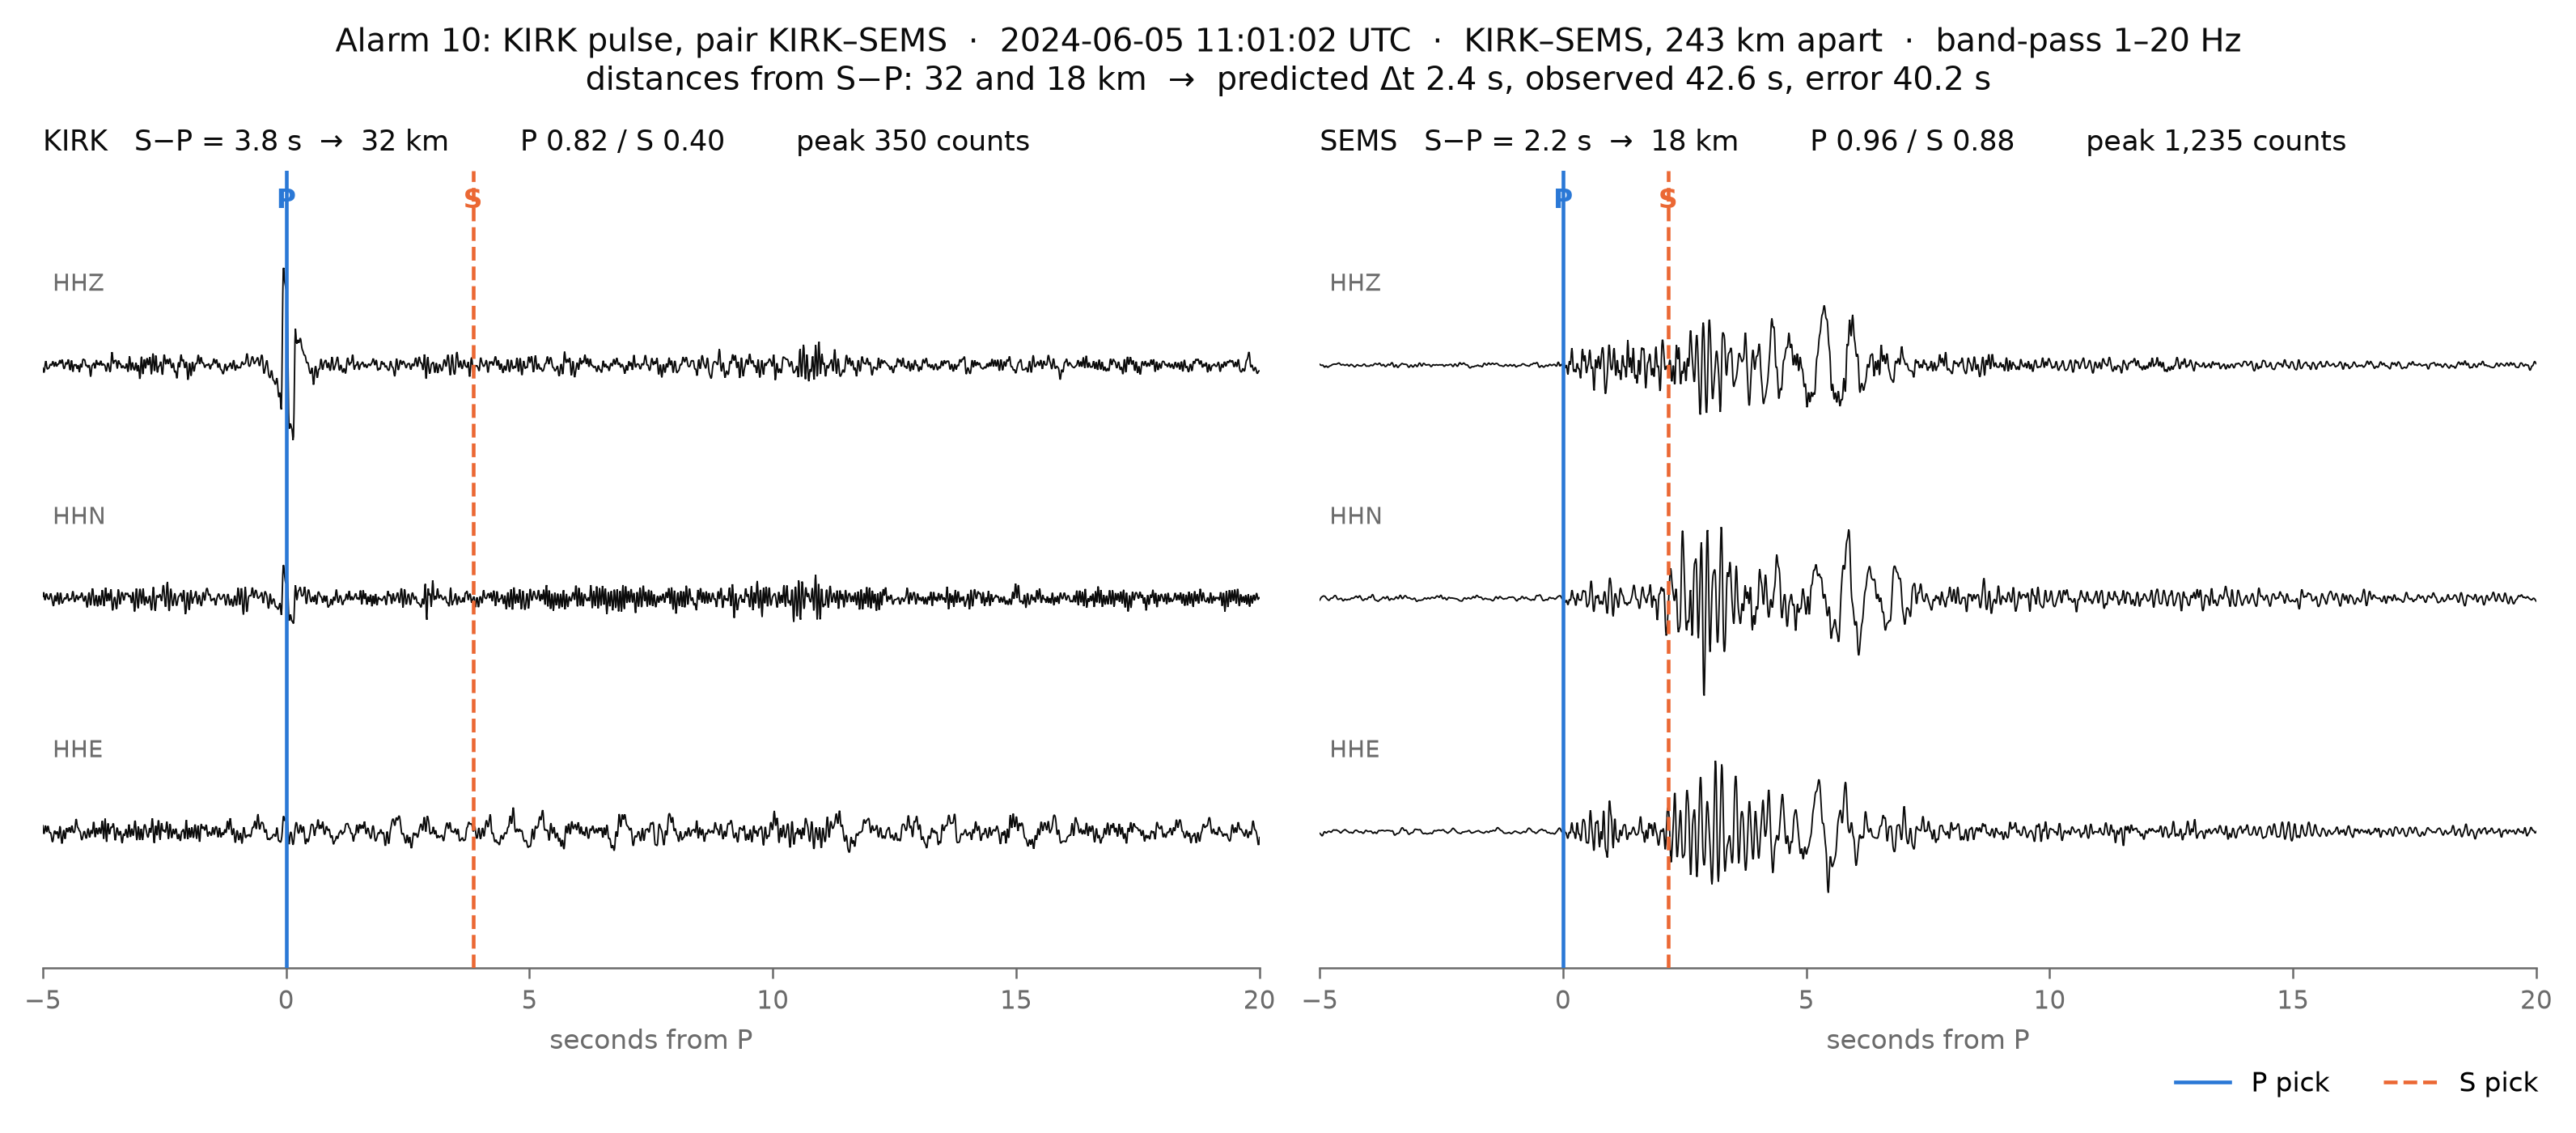
\includegraphics[width=\textwidth]{figures/supp/alarm10_KIRK_SEMS.png}
  \caption*{Alarm 10: KIRK pulse, pair KIRK–SEMS.}
\end{figure}
\begin{figure}[p]\centering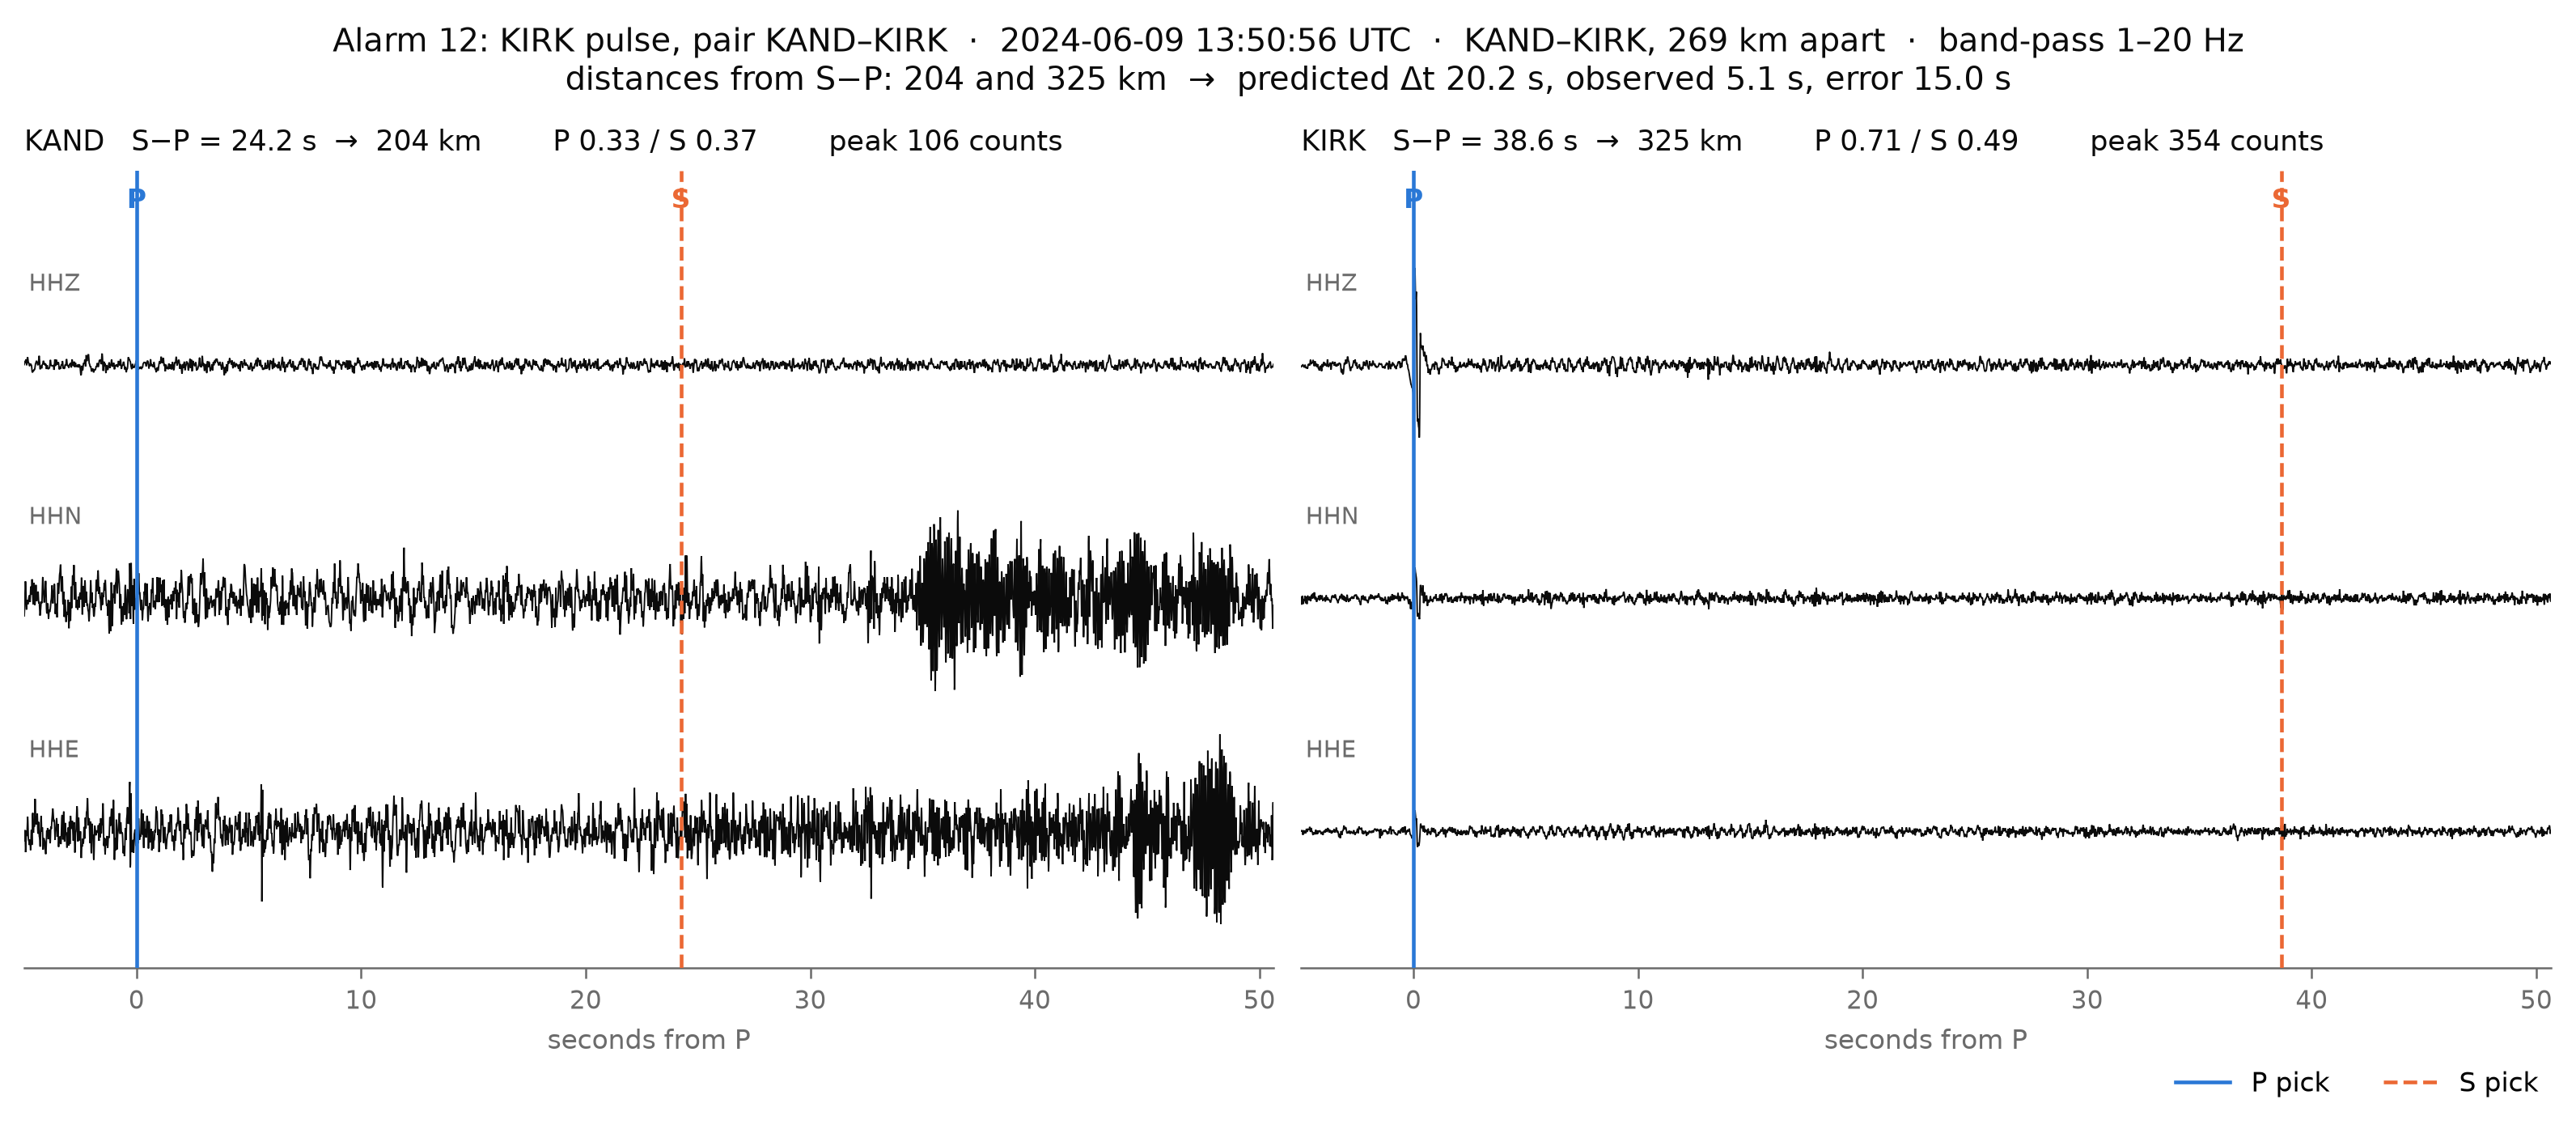
\includegraphics[width=\textwidth]{figures/supp/alarm12_KAND_KIRK.png}
  \caption*{Alarm 12: KIRK pulse, pair KAND–KIRK.}
\end{figure}
\begin{figure}[p]\centering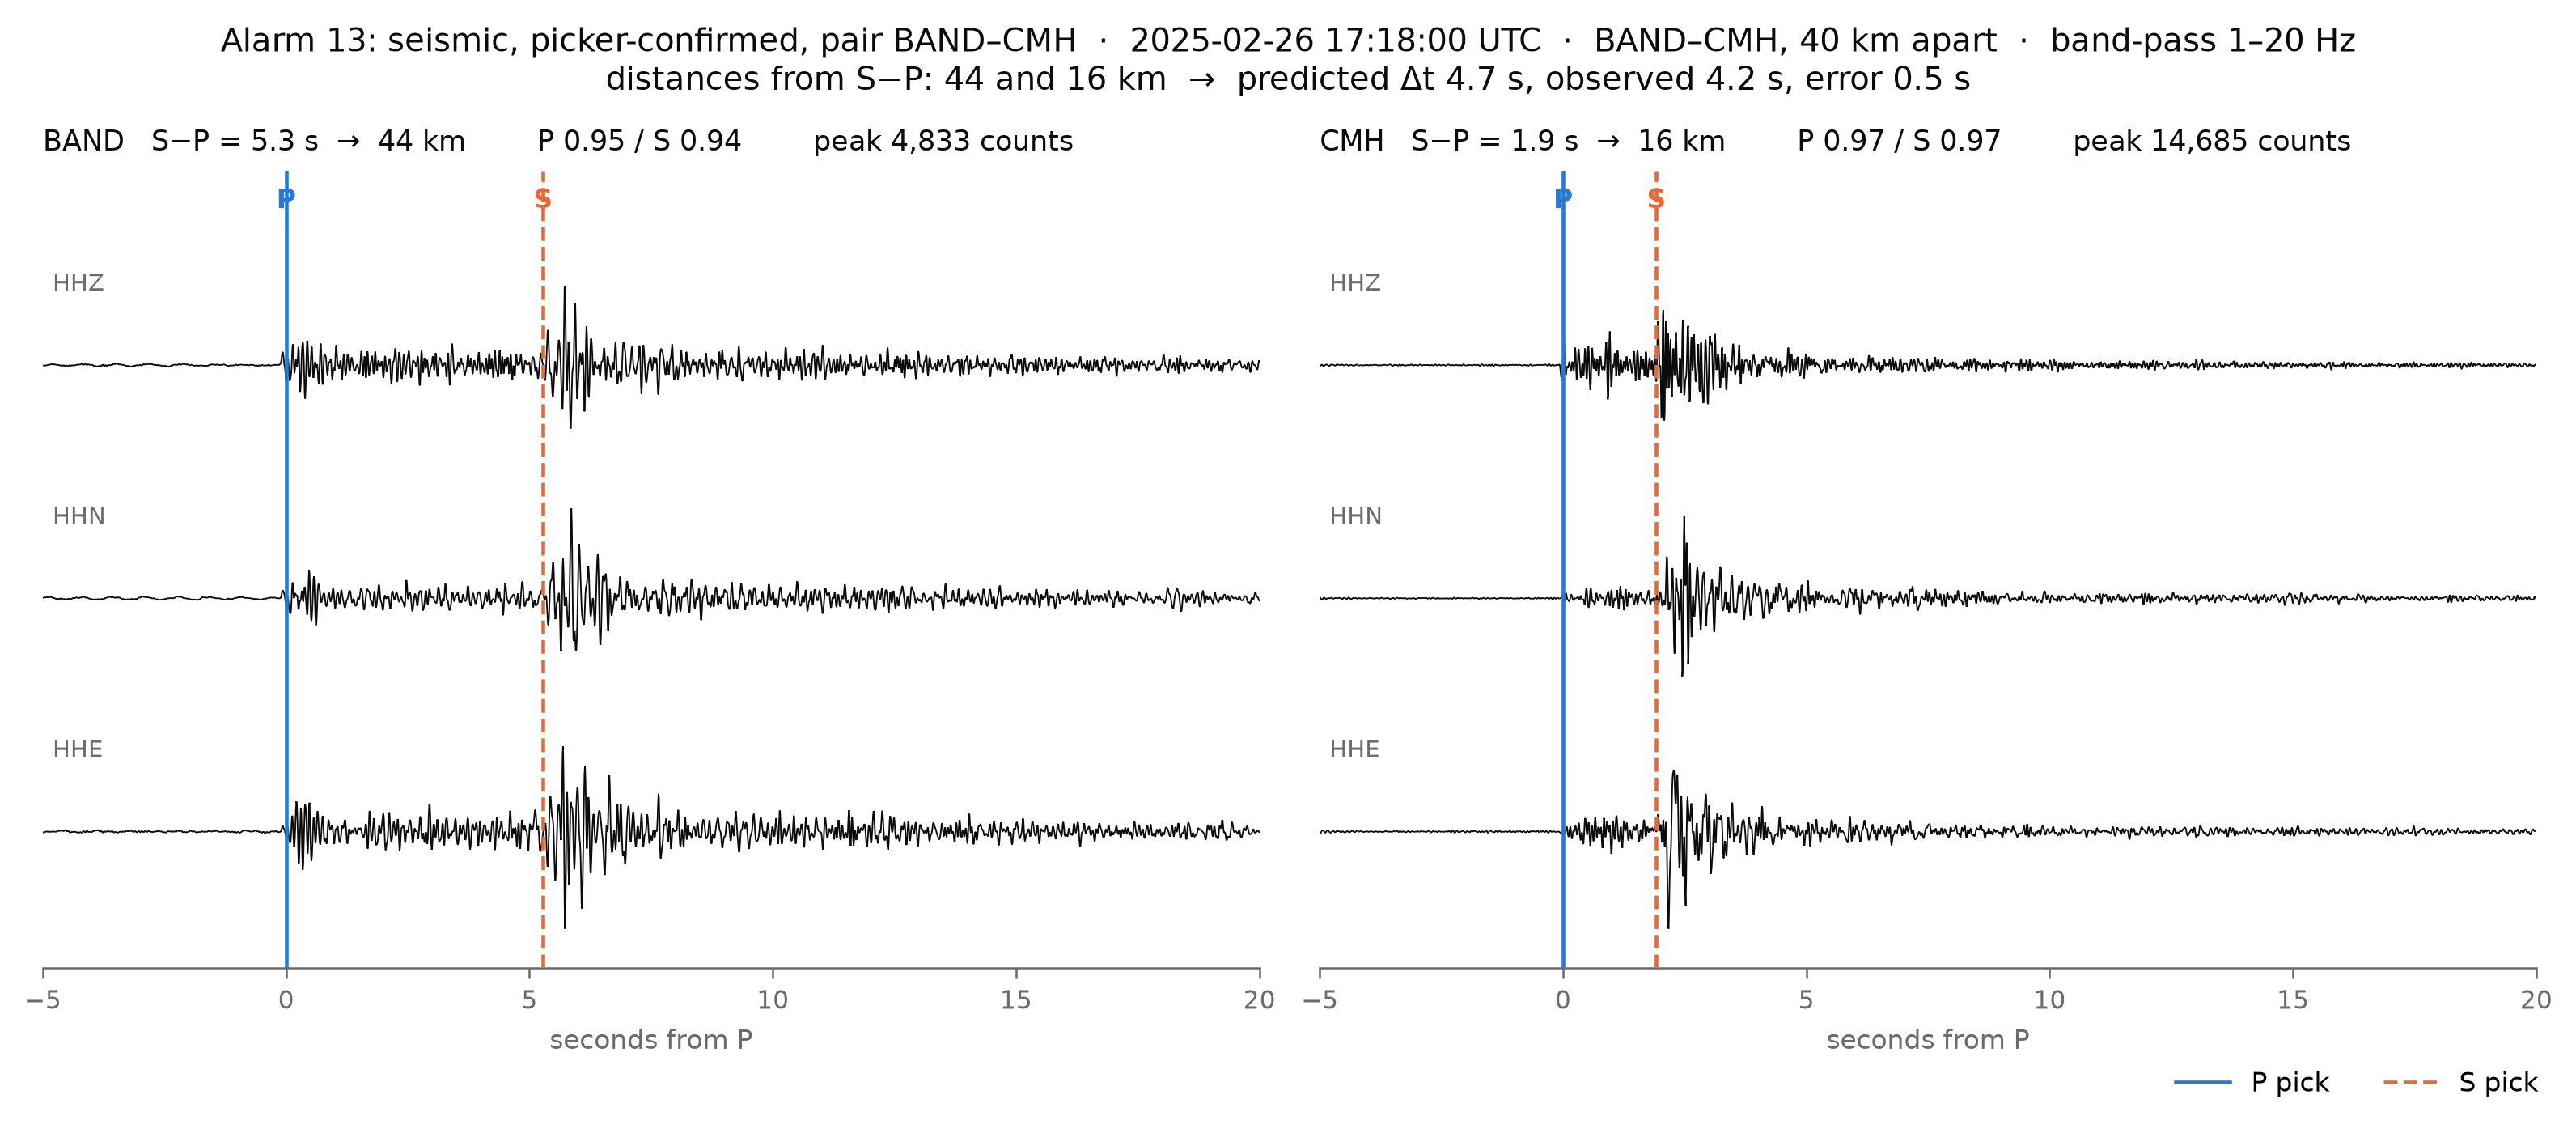
\includegraphics[width=\textwidth]{figures/supp/alarm13_BAND_CMH.png}
  \caption*{Alarm 13: seismic, picker-confirmed, pair BAND–CMH.}
\end{figure}
\begin{figure}[p]\centering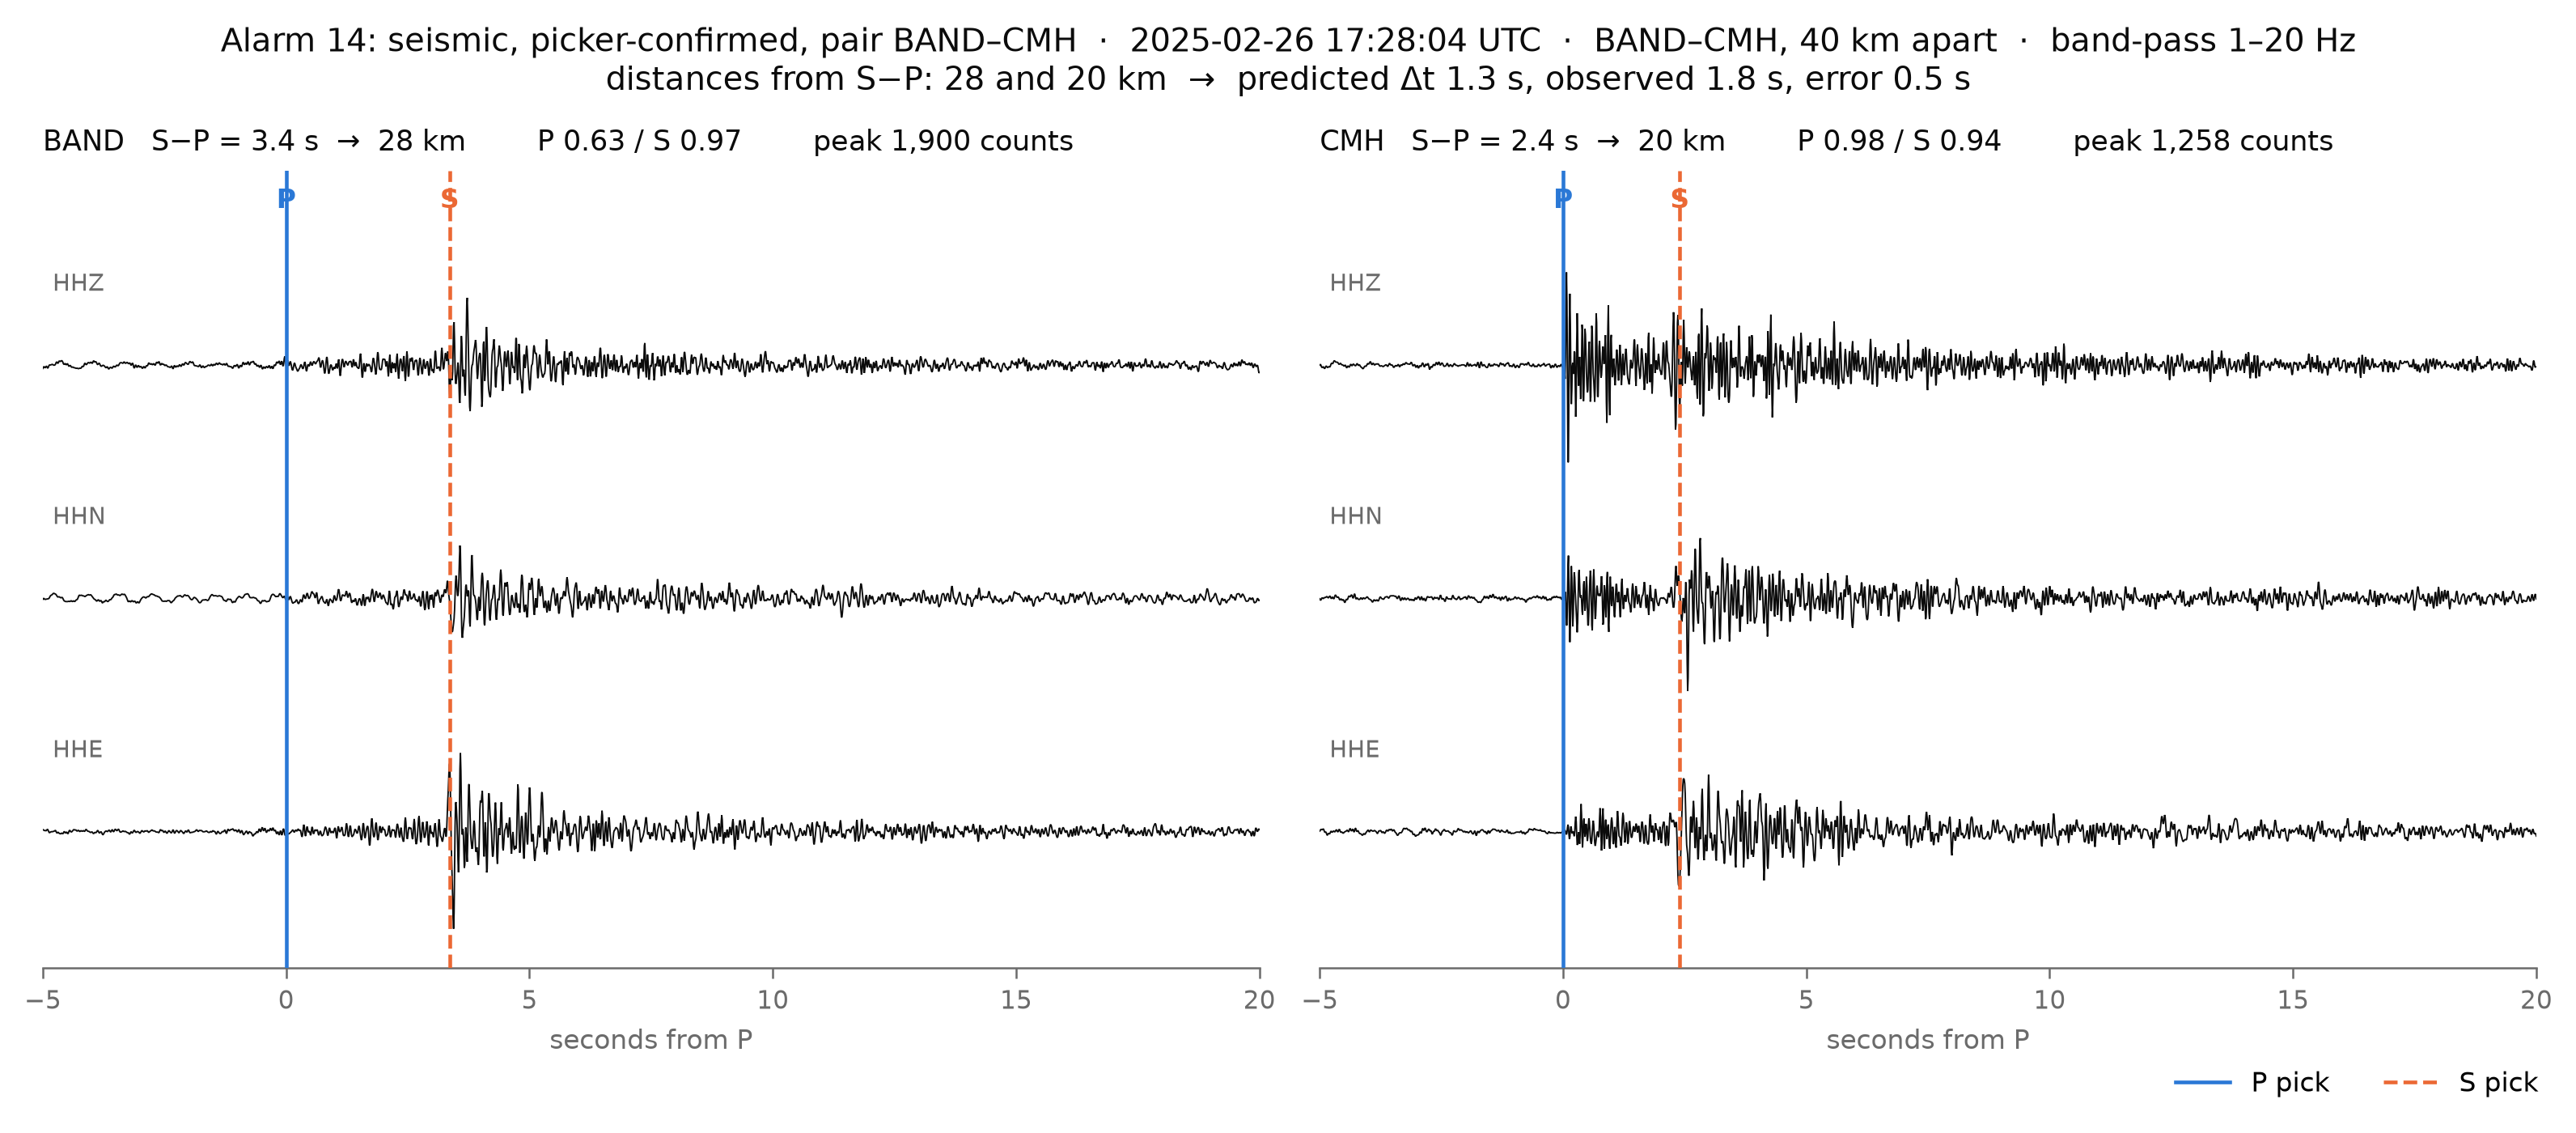
\includegraphics[width=\textwidth]{figures/supp/alarm14_BAND_CMH.png}
  \caption*{Alarm 14: seismic, picker-confirmed, pair BAND–CMH.}
\end{figure}
\begin{figure}[p]\centering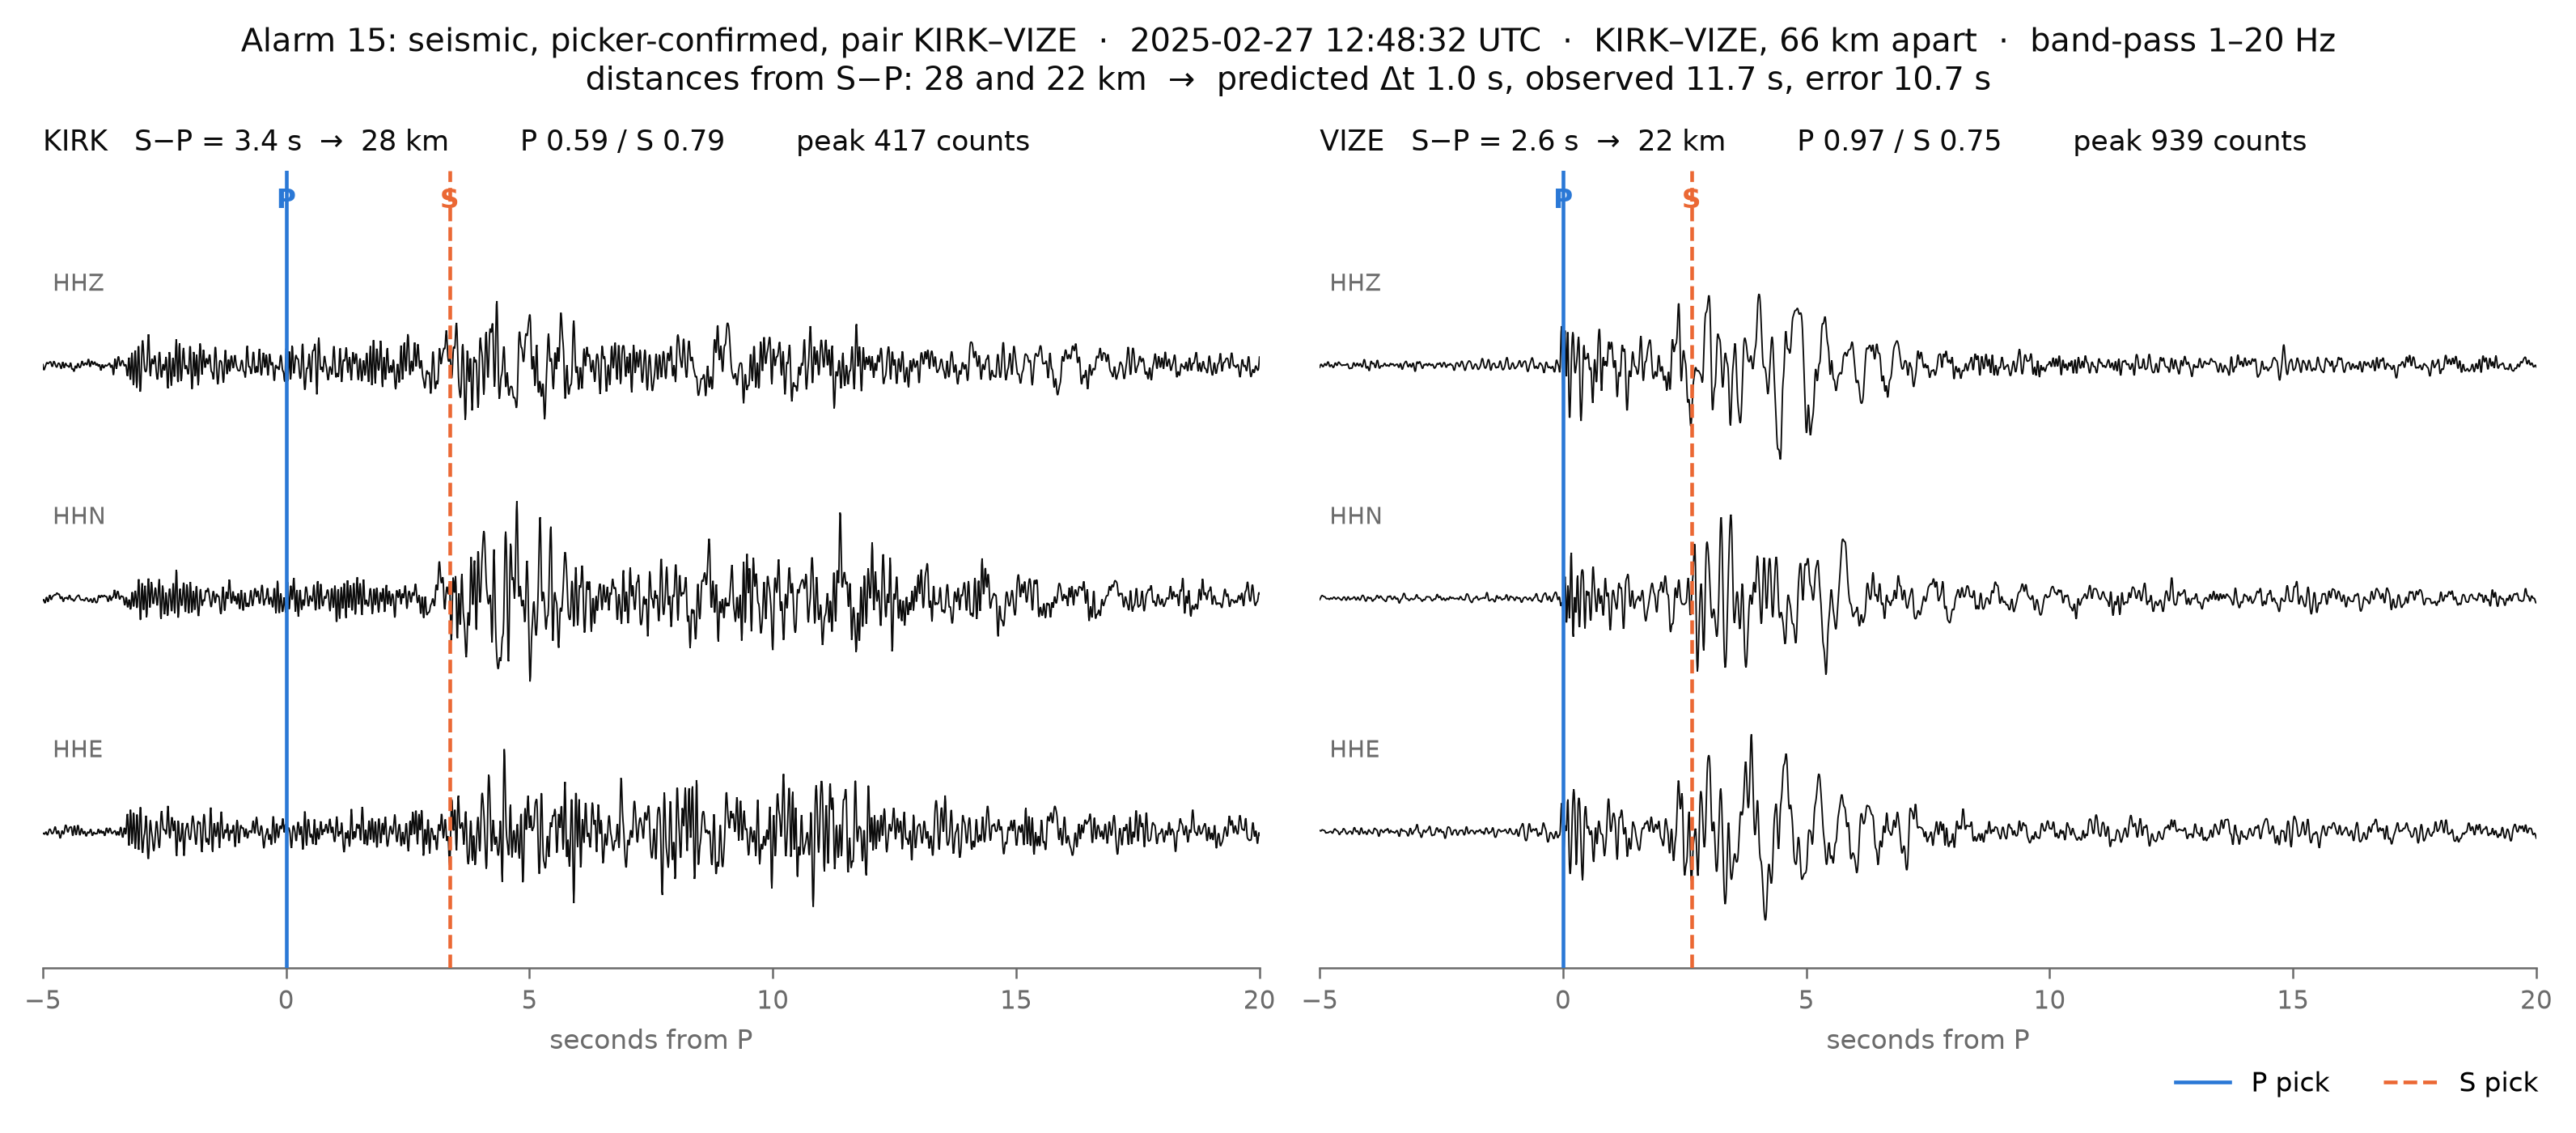
\includegraphics[width=\textwidth]{figures/supp/alarm15_KIRK_VIZE.png}
  \caption*{Alarm 15: seismic, picker-confirmed, pair KIRK–VIZE.}
\end{figure}
\begin{figure}[p]\centering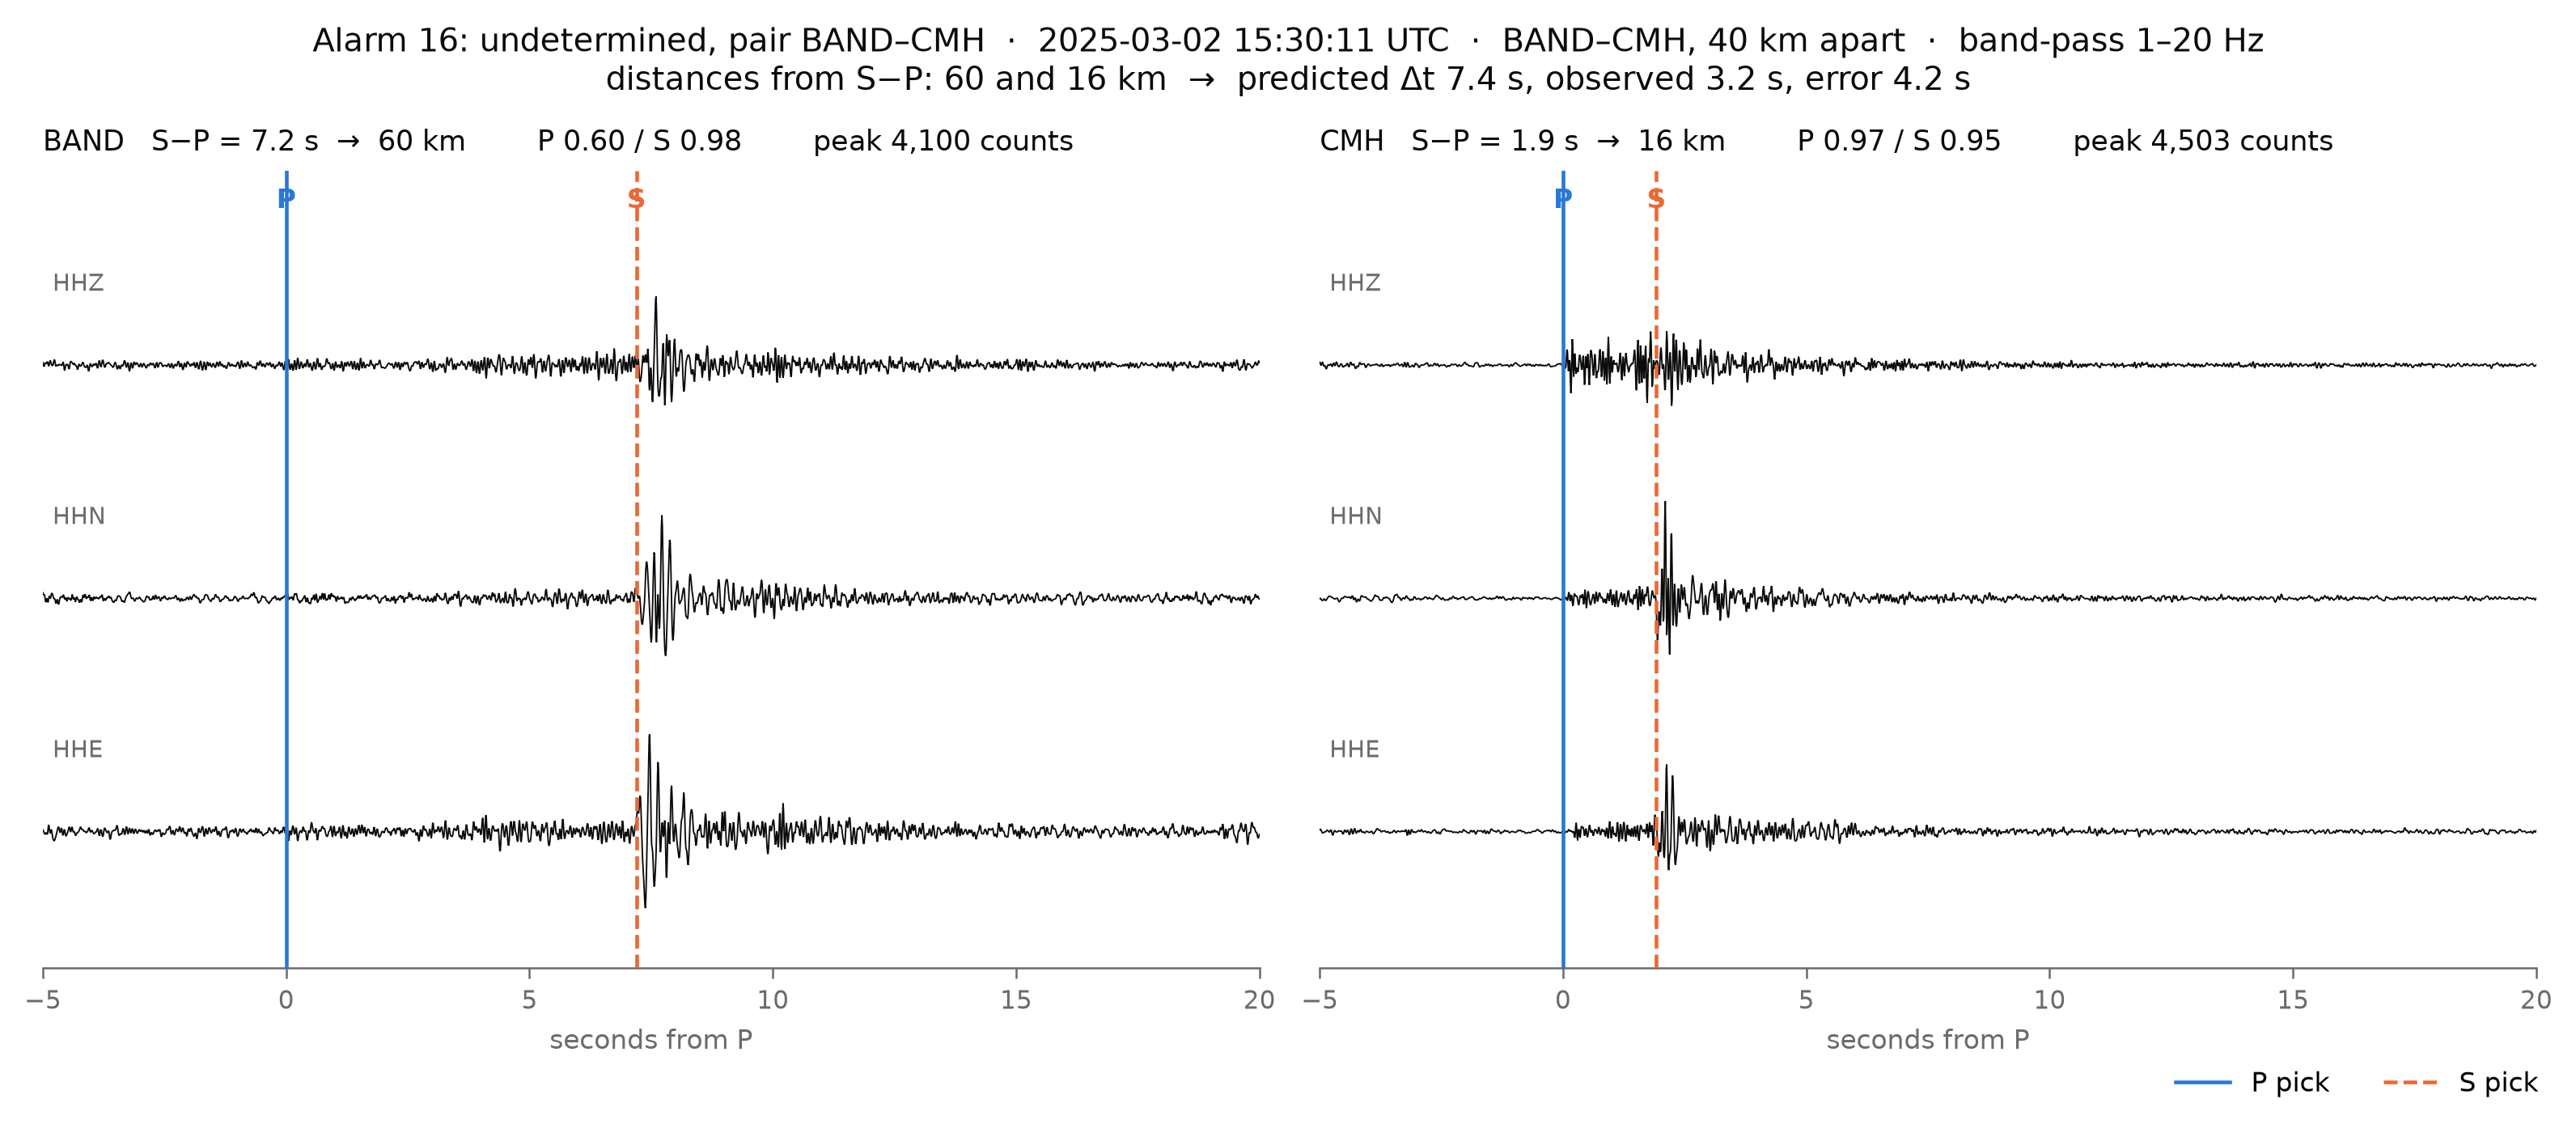
\includegraphics[width=\textwidth]{figures/supp/alarm16_BAND_CMH.png}
  \caption*{Alarm 16: undetermined, pair BAND–CMH.}
\end{figure}
\clearpage
\begin{figure}[p]\centering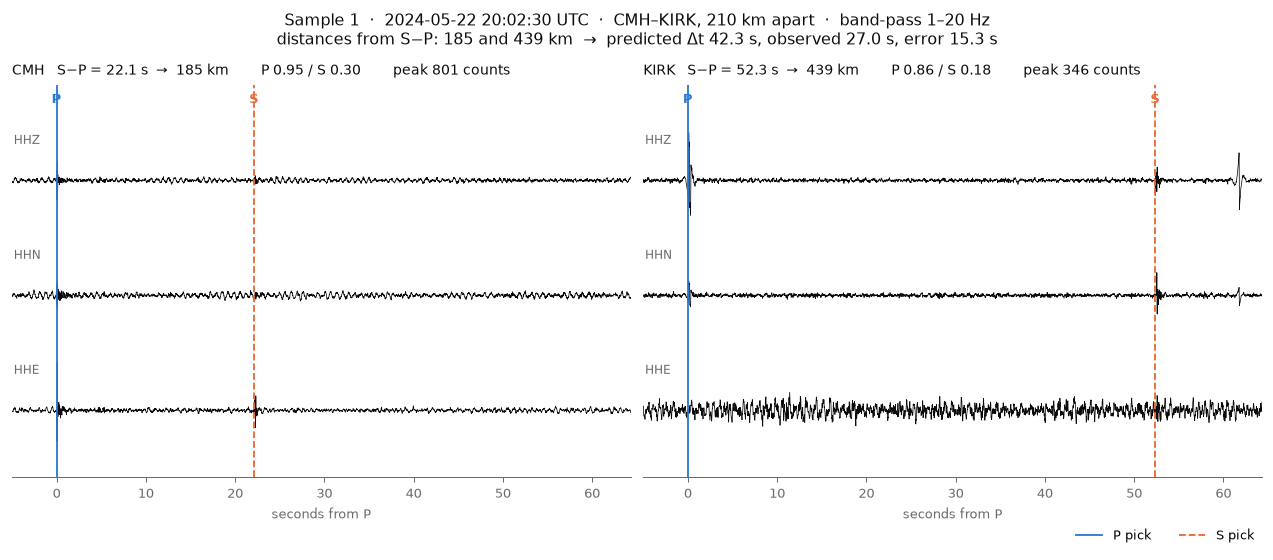
\includegraphics[width=\textwidth]{figures/supp/stalta_sample_1_20240522_1924_CMH_KIRK.png}
  \caption*{\stalta{}; window 20240522~1924; CMH--KIRK; random sample.}
\end{figure}
\begin{figure}[p]\centering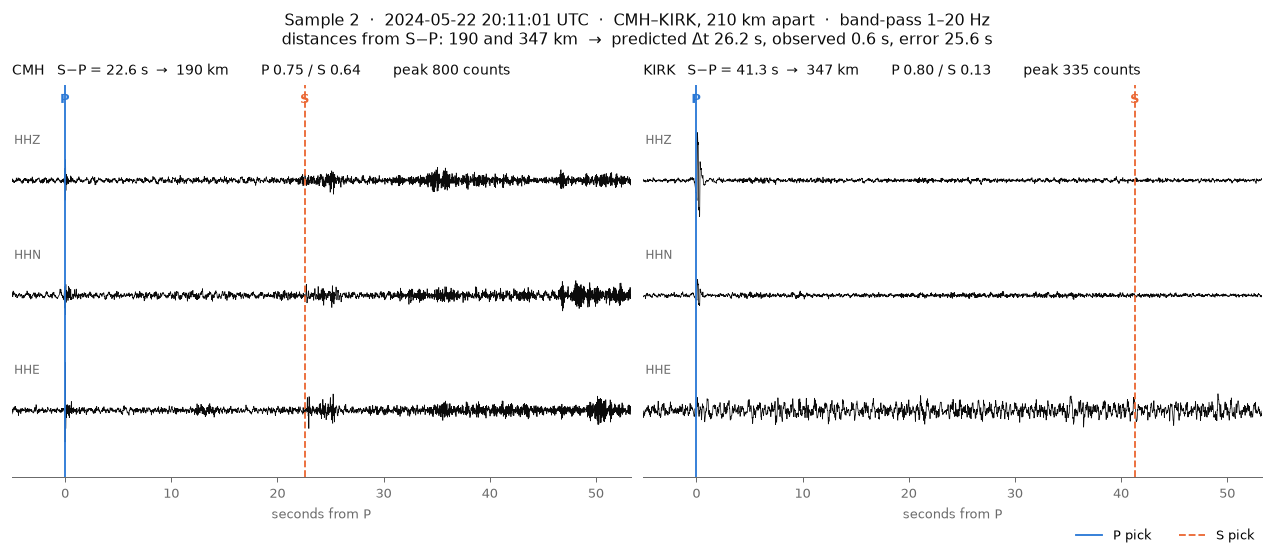
\includegraphics[width=\textwidth]{figures/supp/stalta_sample_2_20240522_1924_CMH_KIRK.png}
  \caption*{\stalta{}; window 20240522~1924; CMH--KIRK; random sample.}
\end{figure}
\begin{figure}[p]\centering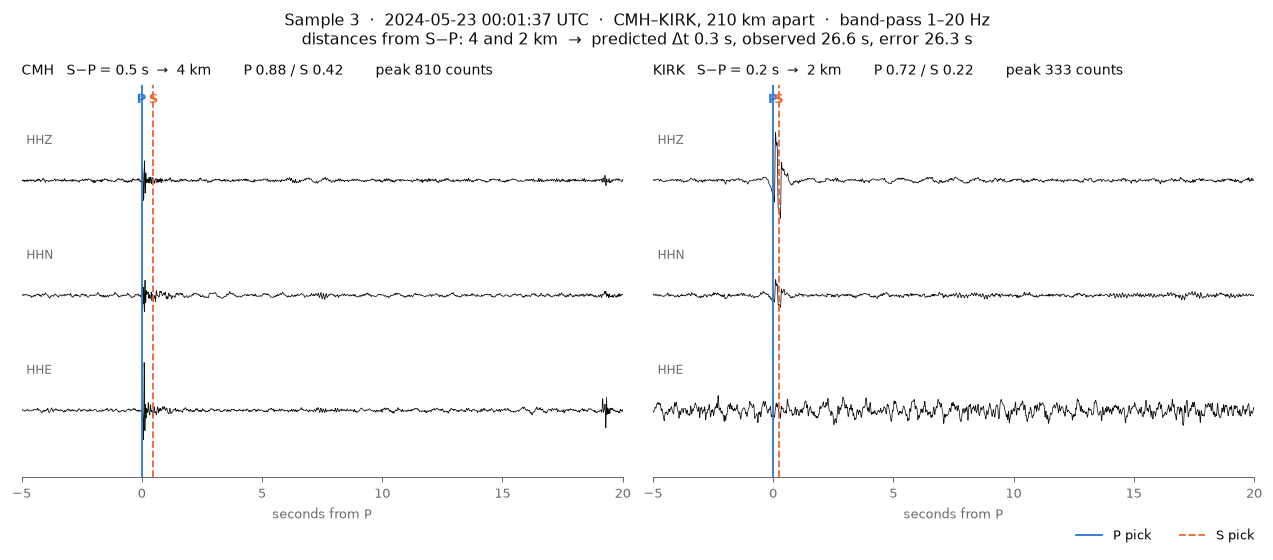
\includegraphics[width=\textwidth]{figures/supp/stalta_sample_3_20240522_1924_CMH_KIRK.png}
  \caption*{\stalta{}; window 20240522~1924; CMH--KIRK; random sample.}
\end{figure}
\begin{figure}[p]\centering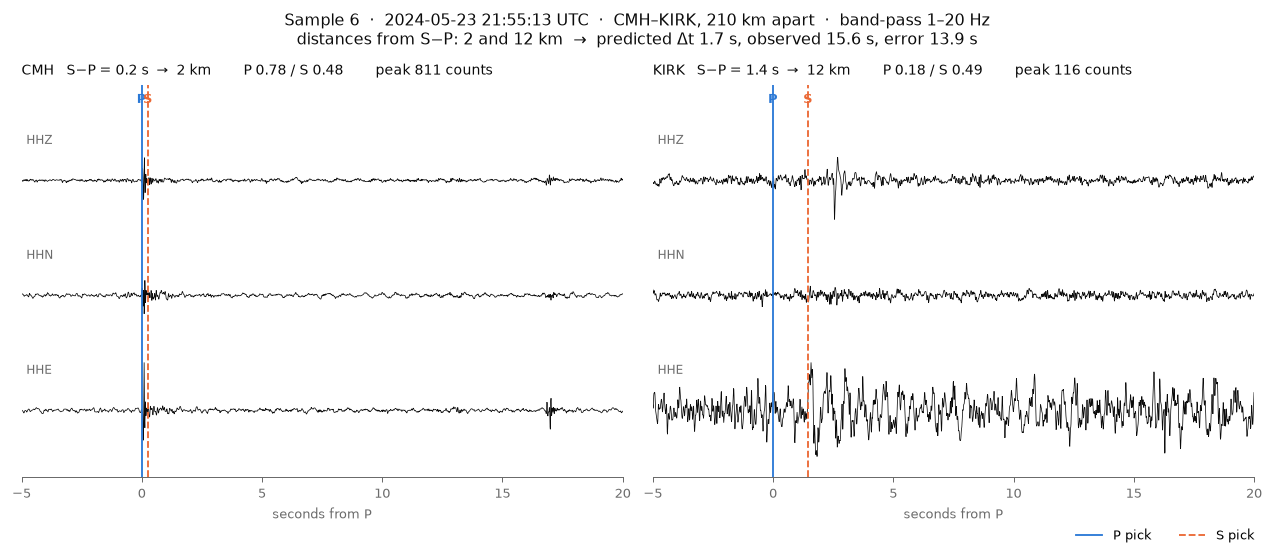
\includegraphics[width=\textwidth]{figures/supp/stalta_sample_6_20240523_2121_CMH_KIRK.png}
  \caption*{\stalta{}; window 20240523~2121; CMH--KIRK; random sample.}
\end{figure}
\begin{figure}[p]\centering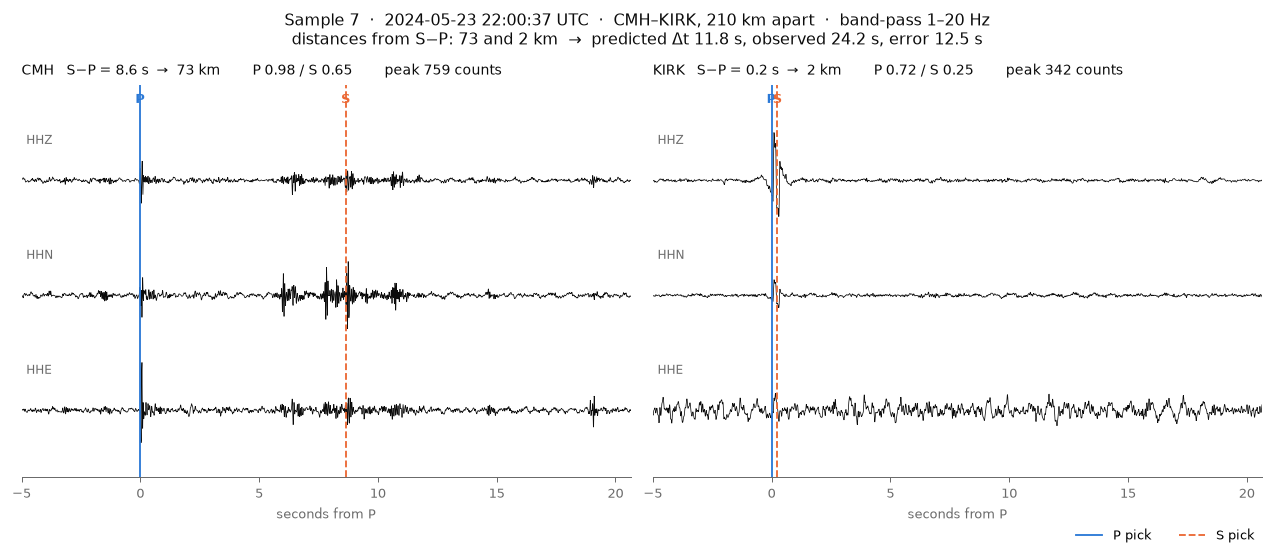
\includegraphics[width=\textwidth]{figures/supp/stalta_sample_7_20240523_2121_CMH_KIRK.png}
  \caption*{\stalta{}; window 20240523~2121; CMH--KIRK; random sample.}
\end{figure}
\begin{figure}[p]\centering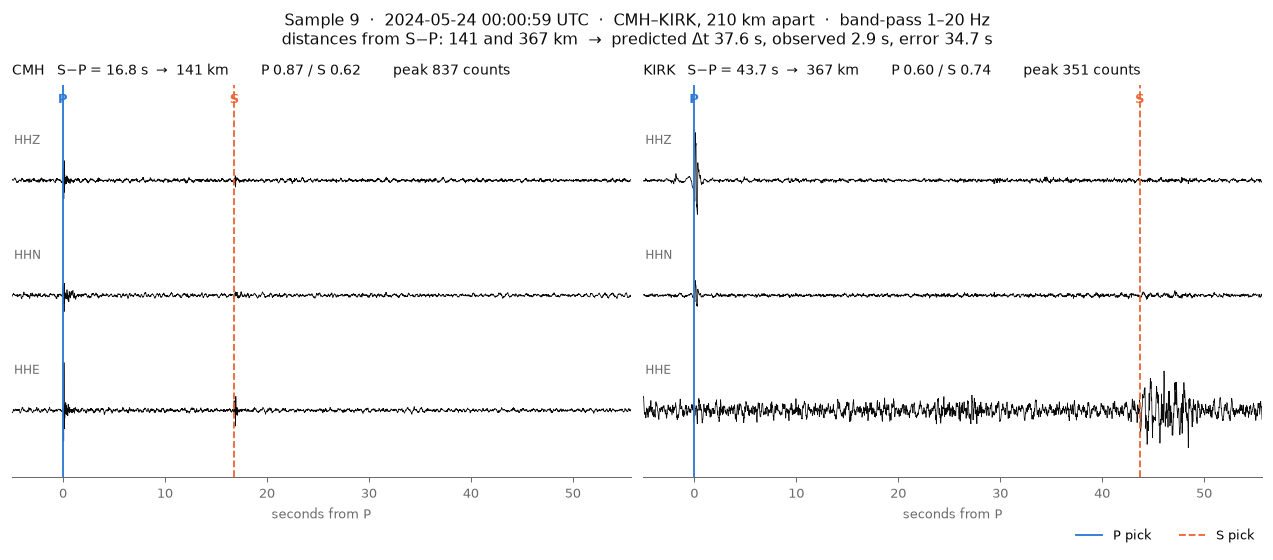
\includegraphics[width=\textwidth]{figures/supp/stalta_sample_9_20240523_2121_CMH_KIRK.png}
  \caption*{\stalta{}; window 20240523~2121; CMH--KIRK; random sample.}
\end{figure}
\begin{figure}[p]\centering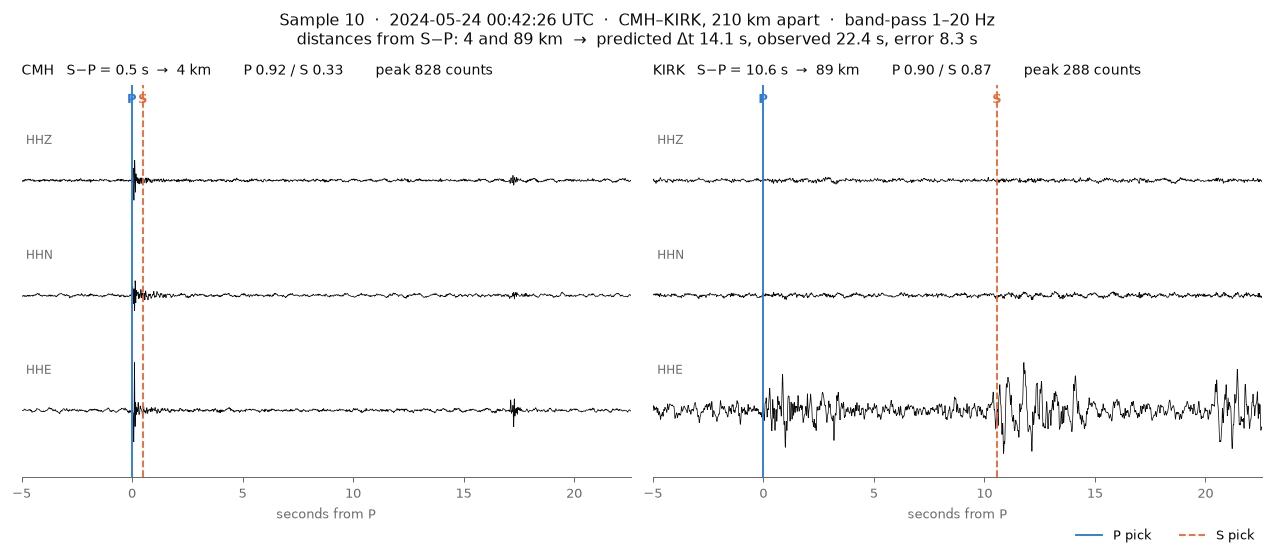
\includegraphics[width=\textwidth]{figures/supp/stalta_sample_10_20240523_2121_CMH_KIRK.png}
  \caption*{\stalta{}; window 20240523~2121; CMH--KIRK; random sample.}
\end{figure}
\begin{figure}[p]\centering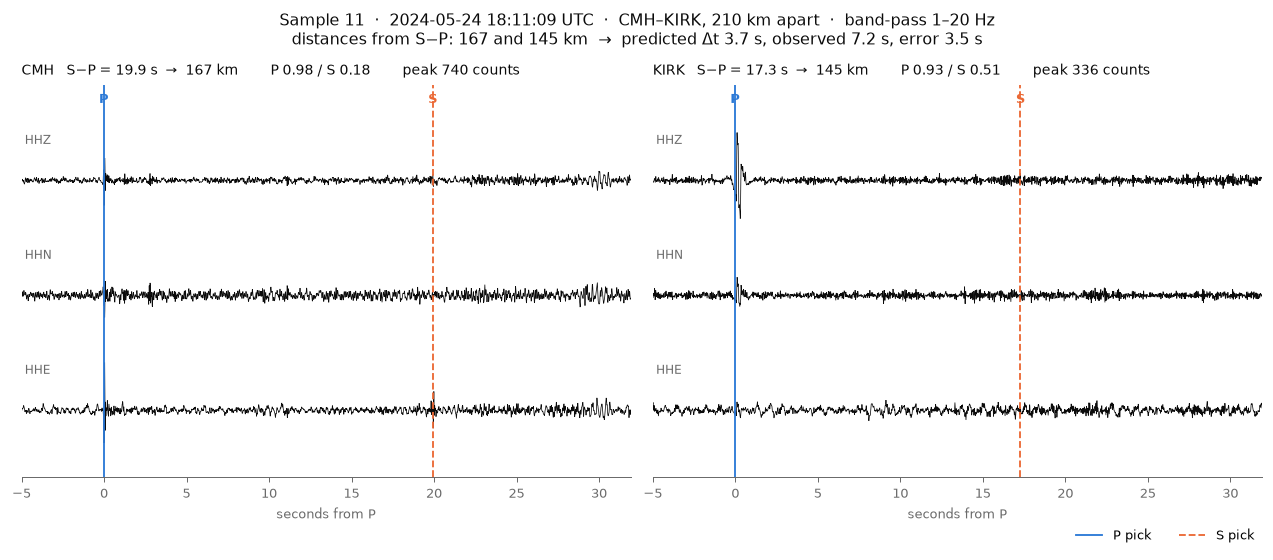
\includegraphics[width=\textwidth]{figures/supp/stalta_sample_11_20240524_1450_CMH_KIRK.png}
  \caption*{\stalta{}; window 20240524~1450; CMH--KIRK; random sample.}
\end{figure}
\begin{figure}[p]\centering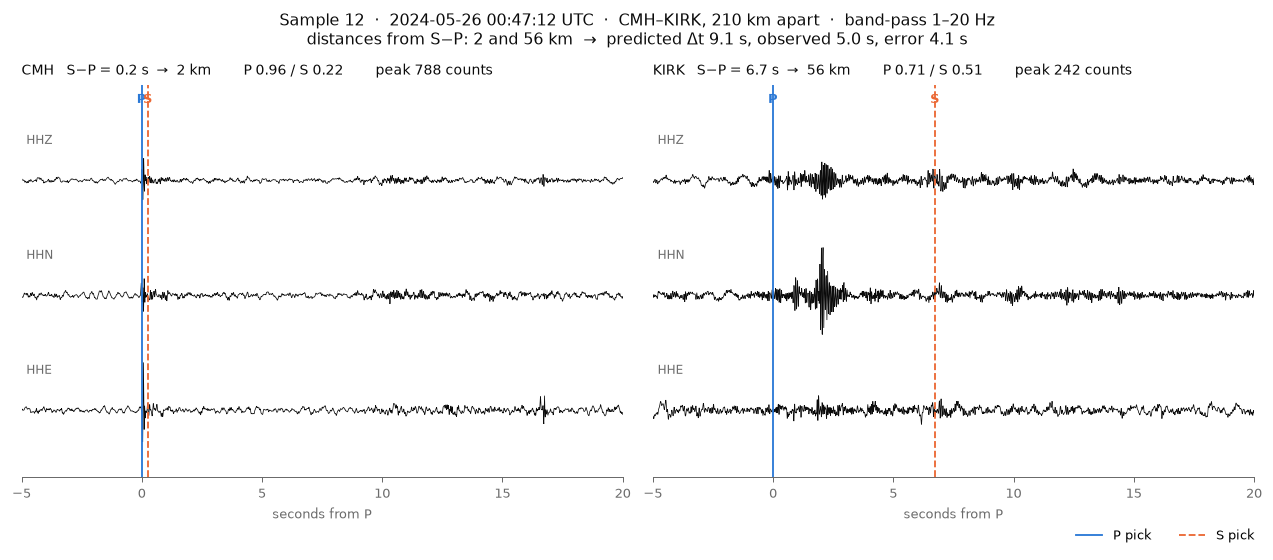
\includegraphics[width=\textwidth]{figures/supp/stalta_sample_12_20240526_0001_CMH_KIRK.png}
  \caption*{\stalta{}; window 20240526~0001; CMH--KIRK; random sample.}
\end{figure}
\begin{figure}[p]\centering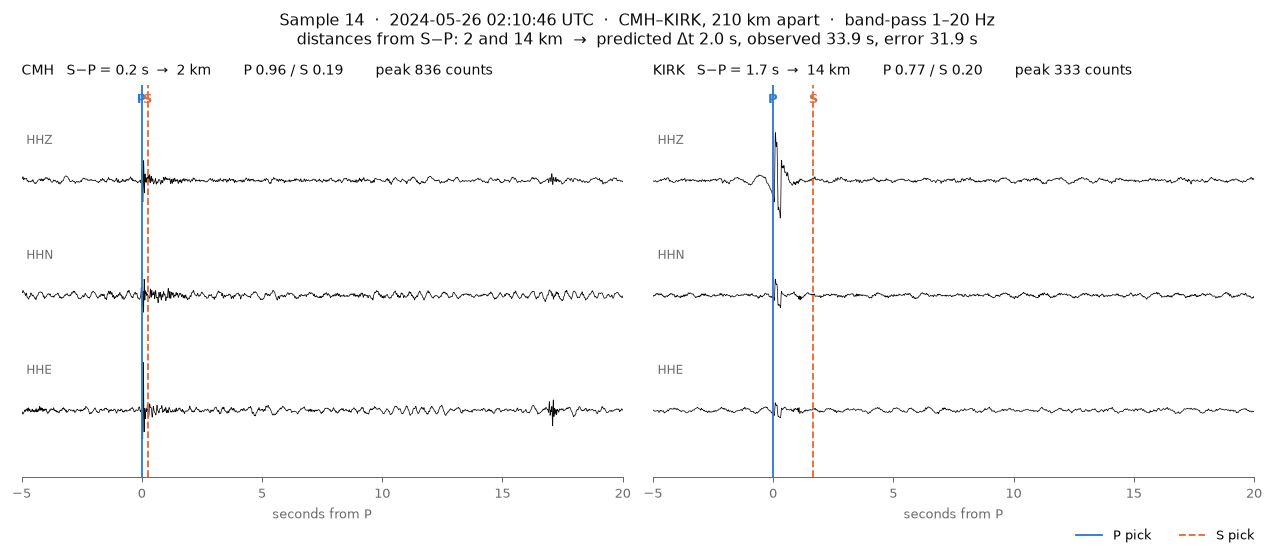
\includegraphics[width=\textwidth]{figures/supp/stalta_sample_14_20240526_0001_CMH_KIRK.png}
  \caption*{\stalta{}; window 20240526~0001; CMH--KIRK; random sample.}
\end{figure}
\begin{figure}[p]\centering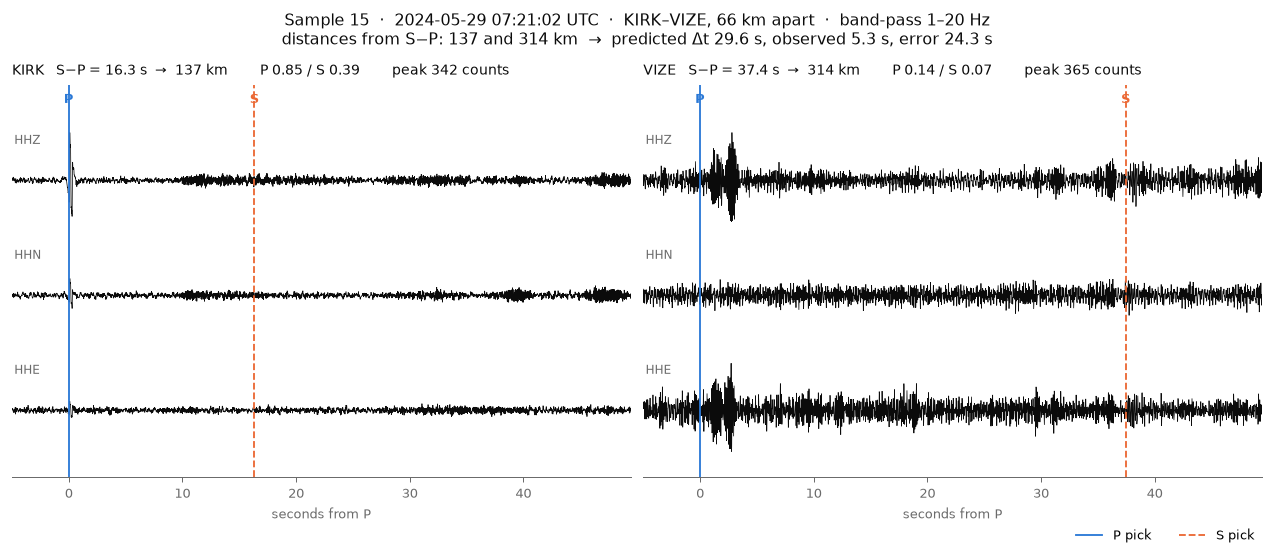
\includegraphics[width=\textwidth]{figures/supp/stalta_sample_15_20240529_0638_KIRK_VIZE.png}
  \caption*{\stalta{}; window 20240529~0638; KIRK--VIZE; random sample.}
\end{figure}
\begin{figure}[p]\centering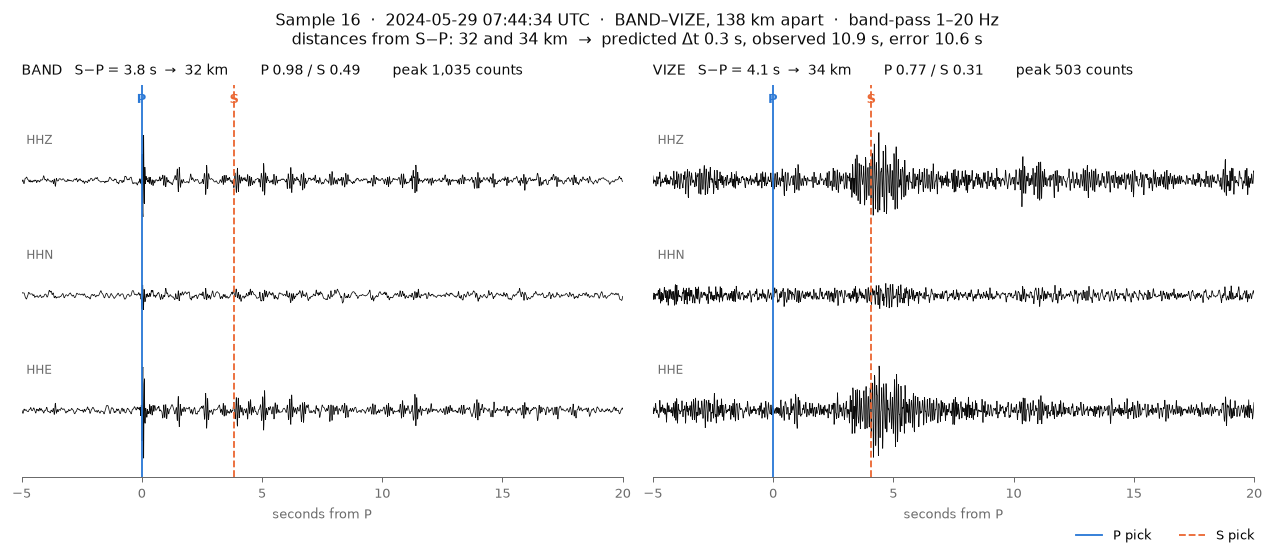
\includegraphics[width=\textwidth]{figures/supp/stalta_sample_16_20240529_0638_BAND_VIZE.png}
  \caption*{\stalta{}; window 20240529~0638; BAND--VIZE; random sample.}
\end{figure}
\begin{figure}[p]\centering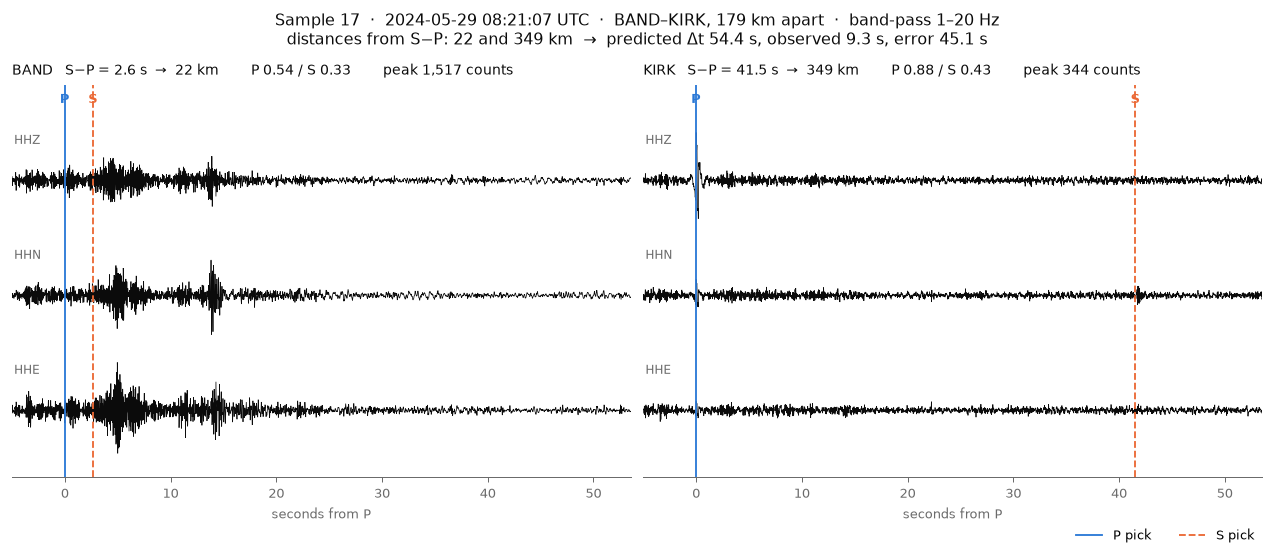
\includegraphics[width=\textwidth]{figures/supp/stalta_sample_17_20240529_0638_BAND_KIRK.png}
  \caption*{\stalta{}; window 20240529~0638; BAND--KIRK; random sample.}
\end{figure}
\begin{figure}[p]\centering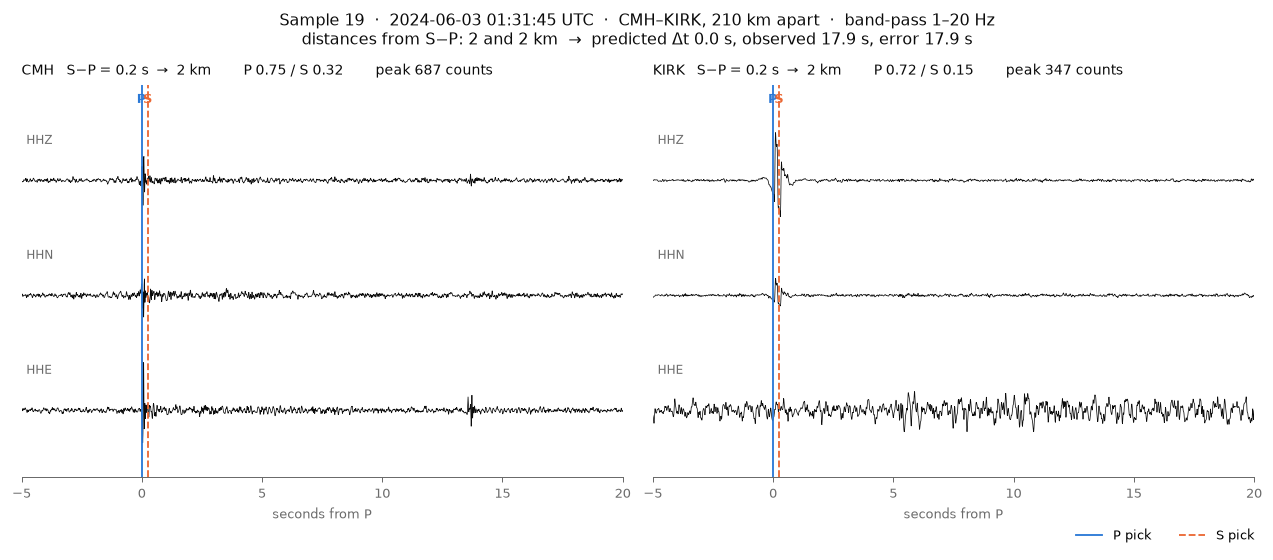
\includegraphics[width=\textwidth]{figures/supp/stalta_sample_19_20240602_2300_CMH_KIRK.png}
  \caption*{\stalta{}; window 20240602~2300; CMH--KIRK; random sample.}
\end{figure}
\begin{figure}[p]\centering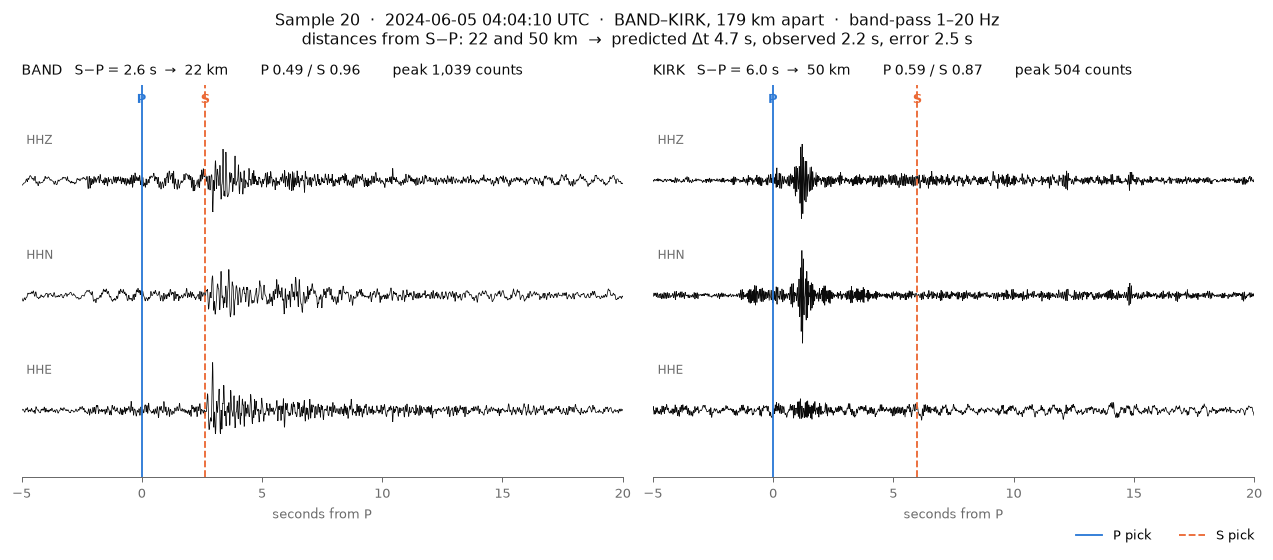
\includegraphics[width=\textwidth]{figures/supp/stalta_sample_20_20240605_0140_BAND_KIRK.png}
  \caption*{\stalta{}; window 20240605~0140; BAND--KIRK; random sample.}
\end{figure}
\begin{figure}[p]\centering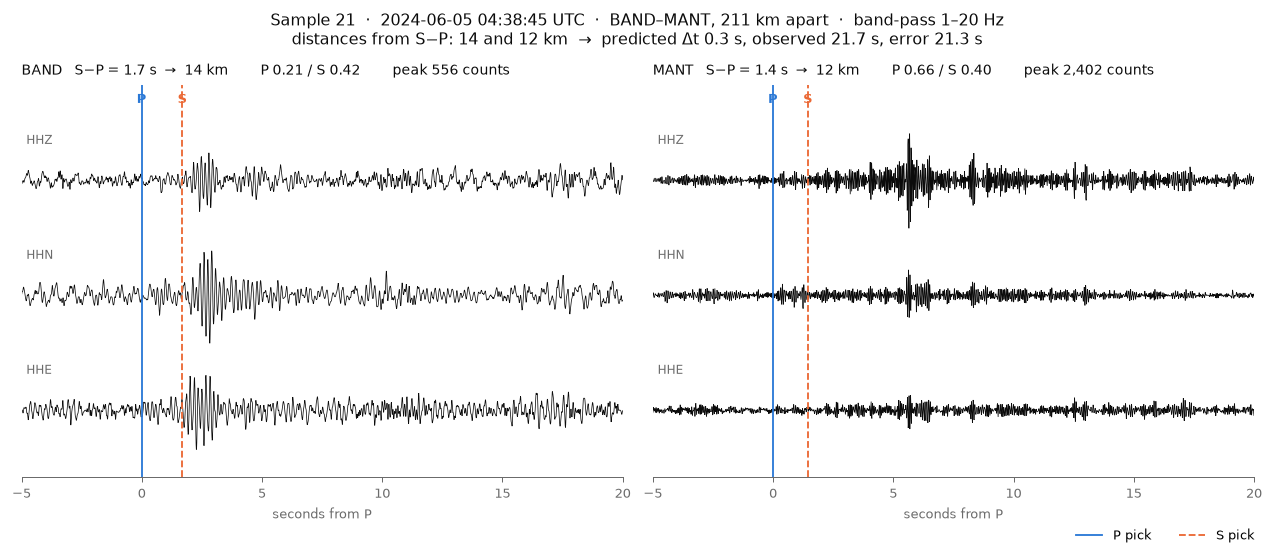
\includegraphics[width=\textwidth]{figures/supp/stalta_sample_21_20240605_0140_BAND_MANT.png}
  \caption*{\stalta{}; window 20240605~0140; BAND--MANT; random sample.}
\end{figure}
\begin{figure}[p]\centering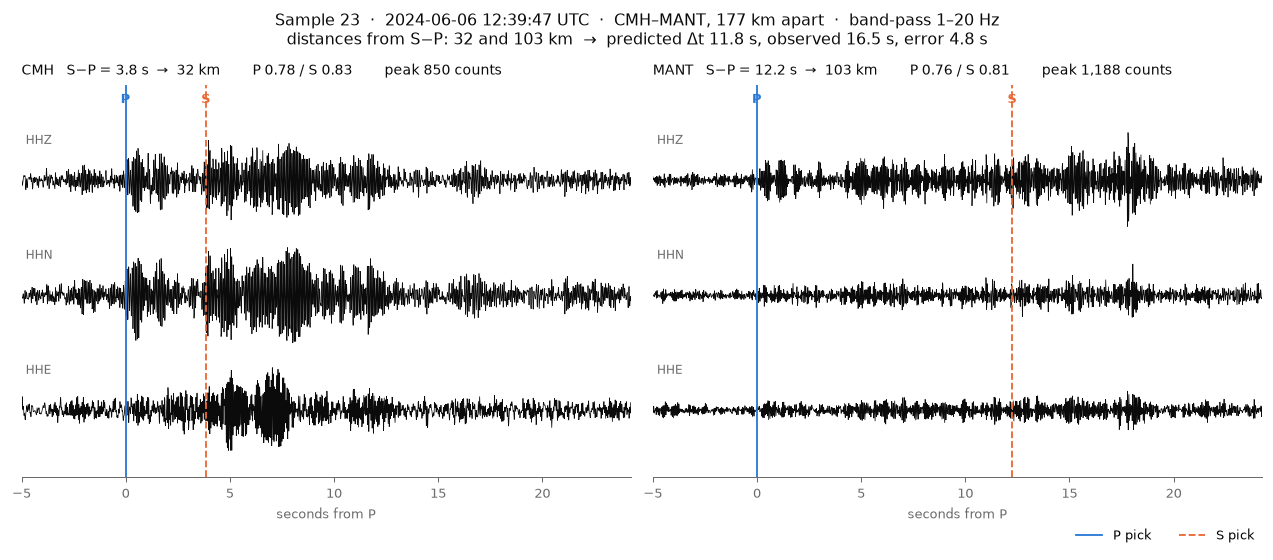
\includegraphics[width=\textwidth]{figures/supp/stalta_sample_23_20240606_1024_CMH_MANT.png}
  \caption*{\stalta{}; window 20240606~1024; CMH--MANT; random sample.}
\end{figure}
\begin{figure}[p]\centering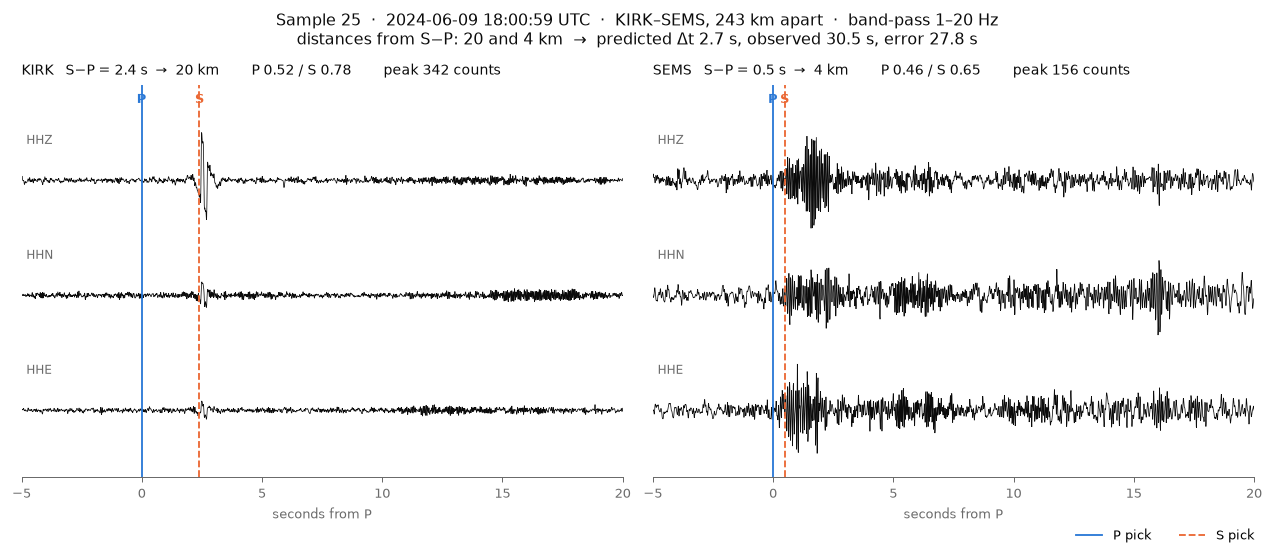
\includegraphics[width=\textwidth]{figures/supp/stalta_sample_25_20240609_1210_KIRK_SEMS.png}
  \caption*{\stalta{}; window 20240609~1210; KIRK--SEMS; random sample.}
\end{figure}
\begin{figure}[p]\centering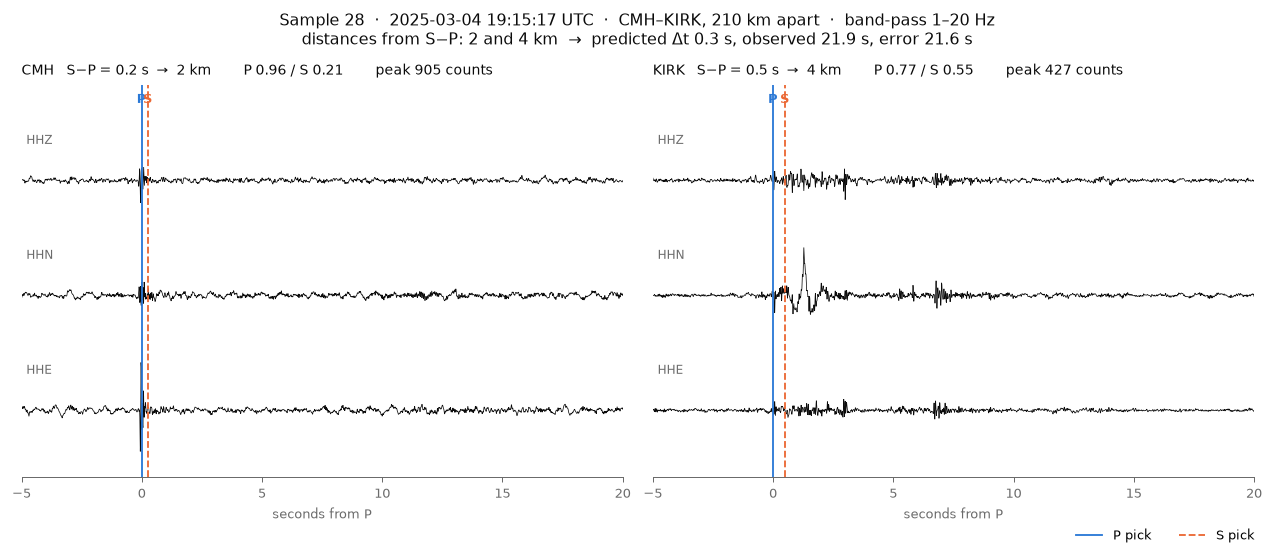
\includegraphics[width=\textwidth]{figures/supp/stalta_sample_28_20250304_1830_CMH_KIRK.png}
  \caption*{\stalta{}; window 20250304~1830; CMH--KIRK; random sample.}
\end{figure}

% ---------------------------------------------------------------------------
\clearpage
\section{FilterPicker: verification, grid and selection}\label{s:filterpicker}

The pipeline's FilterPicker is a port of Lomax's FilterPicker5 v5.0.3 (C). The
test \tool{tests/test_filterpicker.cpp} builds Lomax's code unchanged and compares
the two on synthetic data and on 4~min of DEMI under three parameter sets, and every pick and every sample of the characteristic function agree. The detector runs on
the vertical component; every pick triggers, at most once per 15~s per station,
with P at the pick time and no \stalta{} anchoring, and everything downstream
(picker, association with two stations and a 3~s slack, catalog scoring) is
the pipeline's.

The protocol was committed before the tuning grid was run (Section~\ref{s:prereg}).
Two runs preceded it as checks of the port, both on tuning data at the published defaults. They replayed the AFAD S\i{}nd\i{}rg\i{} half hour on all seven stations of its data directory, and the Marmara replay. The grid on the tuning replays crossed two sets
of windows (filter, long-term and $T_\mathrm{up}$: 3, 5 and 0.2~s, the values of
  Lomax et al.\ (2012) at 100~Hz; 6, 10 and 0.4~s, those of Earthworm's
\texttt{pick\_FP} at 100~Hz) with trigger thresholds of 3, 4, 5, 6, 8, 10, 12, 15
and 20 and acceptance thresholds of 3, 4, 6, 8, 10, 15 and 20 (126 settings), each
scored at the catalog times and the six shifts. The two rules of the main text
were applied against the learned detector's tuning figures (48.7 chance-corrected
detections, 26 unmatched alarms); ties went to fewer unmatched alarms and then to
higher thresholds (equal unmatched), or to more detections (equal detections).

\begin{table}[htbp]
  \centering\footnotesize\setlength{\tabcolsep}{4pt}
  \caption{FilterPicker on the tuning replays (S\i{}nd\i{}rg\i{} 30~min and Marmara,
  66 catalog events).}\label{t:filterpicker}
  \begin{tabular}{@{}llcccc@{}}
    \toprule
    Setting & Windows (s) & Thresholds & Detected & Chance-corrected & Unmatched \\
    \midrule
    equal unmatched (selected)  & 6 / 10 / 0.4 & 15, 10 & 46 & 42.3 & 25 \\
    equal detections (selected) & 3 / 5 / 0.2  & 4, 10  & 53 & 49.8 & 52 \\
    published defaults          & 3 / 5 / 0.2  & 10, 10 &    & 47.5 & 78 \\
    published defaults          & 6 / 10 / 0.4 & 10, 10 &    & 41.0 & 30 \\
    \addlinespace
    learned detector            & \multicolumn{2}{l}{$0.8 \times 8$, or 0.9} & 51 & 48.7 & 26 \\
    \bottomrule
  \end{tabular}
\end{table}

\noindent Over the grid, the most chance-corrected detections at a given number of
unmatched alarms are 36.4 at 4, 37.3 at 6, 39.6 at 20, 42.3 at 25, 44.8 at 41 and
49.8 at 52. Both selected settings alarm on the S\i{}nd\i{}rg\i{} \Mw{}~4.9 (+16.6
and +17.3~s after origin) and the Marmara \Mw{}~6.2 (+9.9~s). On the quiet windows
the stations of the equal-unmatched setting's 353 alarms are CMH (300), KIRK
(274), VIZE (45), SEMS (28), MANT (25), BAND (22), ELBA (11) and KAND (1).

\noindent Reproduction: \tool{tools/sweep_trigger.py} with
\texttt{-{}-args '-{}-detector filterpicker'}, \texttt{-{}-set fp-windows=...} and
\texttt{-{}-set fp-thresholds=...};
\tool{tools/select_setting.py} applies the rules; \tool{tools/event_outcomes.py}
and \tool{tools/significance.py} give the paired tests of the main text.

% ---------------------------------------------------------------------------
\clearpage
\section{Record of protocols committed in advance}\label{s:prereg}

Every choice that fixed a setting or an analysis before held-out or quiet data
were scored, with the commit that records it. Commits in \emph{ayzek} are in the
pipeline's repository, the others in the paper's. Times are commit times
(UTC+3), recorded by the authors' own repositories and not timestamped by a third
party; the order of steps therefore rests on these records.

\begin{table}[htbp]
  \centering\footnotesize\setlength{\tabcolsep}{4pt}
  \caption{The steps committed in advance, their records and what preceded each.}\label{t:prereg}
  \begin{tabular}{@{}>{\raggedright\arraybackslash}p{3.6cm}l>{\raggedright\arraybackslash}p{2.3cm}>{\raggedright\arraybackslash}p{6.2cm}@{}}
    \toprule
    Step & Commit & Date & Run before it \\
    \midrule
    learned detector: trigger rule chosen on the tuning replays &
    \emph{ayzek} 500254a & 2026-09-17 02:51 &
    the tuning grid; the first held-out result is in the same commit, and the order therefore rests on the authors' record \\
    \stalta{}: the two selection rules &
    \emph{ayzek} a04dc9c & 2026-09-17 20:49 &
    the tuning grid; the held-out results are in the same commit \\
    published models: protocol & 91b9ee1 & 2026-10-22 16:27 &
    one adapter check on the S\i{}nd\i{}rg\i{} 30~min tuning replay, recorded in
    571ef5f \\
    published models: selection & 4973cb8 & 2026-10-22 17:54 &
    the tuning grid; no held-out, Simav or quiet-window run \\
    second held-out sequence (Simav): protocol & 51067a1 & 2026-10-23 09:49 &
    a list of candidate sequences by catalog counts and station distances;
    no waveform, score or replay \\
    quiet-window alarms: classification rule, PhaseNet & 0a0dff8 & 2026-10-23 10:27 &
    no picker run \\
    quiet-window alarms: EQTransformer cross-check & 8380650 & 2026-10-23 10:36 &
    the PhaseNet run of the rule above \\
    FilterPicker: protocol & 851f3fb & 2026-10-26 20:43 &
    two runs at the published defaults on tuning data (Section~\ref{s:filterpicker}) \\
    FilterPicker: selection & 9580e0f & 2026-10-26 21:15 &
    the tuning grid; no held-out, Simav or quiet-window run \\
    quiet-window alarms: any-pair rule and catalog search & c78517b & 2026-10-27 18:24 &
    no run of either \\
    published models, 1--2~s look-ahead: protocol & 761d22b & 2026-10-27 21:13 &
    one check that \tool{--ahead 0} reproduces the causal scores \\
    published models, 1--2~s look-ahead: selection & a6bdd22 & 2026-10-27 21:58 &
    the tuning grid; no held-out, Simav or quiet-window run \\
    \bottomrule
  \end{tabular}
\end{table}

\noindent The evaluation runs followed the protocols. The published models were evaluated in fba5ffb (2026-10-22 19:16) and the Simav sequence in 49fe24f (2026-10-23 13:01). FilterPicker was evaluated on 2026-10-26 between 21:15 and 21:20, with its results in c06566f, and the look-ahead settings on 2026-10-27 between 22:02 and 23:16, with their results in 40003af.
No setting was changed after any evaluation run.

% ---------------------------------------------------------------------------
\clearpage
\section{The continuous-record ranking without the S wave}\label{s:swave}

Main-text Table~4 scores an event by the highest window score in its guard, from 10~s before the predicted P (minus the window length) to 60~s after it, and every detector can therefore score the S wave and coda as well as the P wave. Here an event
is scored only from windows that end at least a margin before its predicted S
arrival (IASP91), and only events whose S$-$P interval is at least 6~s plus the
margin are counted, so that every detector, including the 6~s detectors on their
6~s grid, has a window ending between P and that limit. Thresholds are those of Table~4, because they are set by the background, which does not depend on how events are scored. The event AUC compares each event's maximum with the maximum over one
random stretch of record of the same length, clear of every cataloged event.

\begin{table}[htbp]
  \centering\footnotesize\setlength{\tabcolsep}{4pt}
  \caption{Recall at three alarm budgets and event AUC on the 728-day MANT record,
    with each event scored over its full guard and only before its S wave (margin
  1~s; 12{,}206 events with SNR~$\geq 3$ and S$-$P~$\geq 7$~s).}\label{t:swave}
  \begin{tabular}{@{}lcccccccc@{}}
    \toprule
    & \multicolumn{4}{c}{Full guard} & \multicolumn{4}{c}{Before the S wave} \\
    \cmidrule(lr){2-5}\cmidrule(lr){6-9}
    Detector & AUC & 100/day & 10/day & 1/day & AUC & 100/day & 10/day & 1/day \\
    \midrule
    \multicolumn{9}{@{}l}{\emph{Run by the pipeline}} \\
    \stalta{} (causal, 2--20~Hz)   & 0.9911 & 0.991 & 0.724 & 0.217 & 0.9889 & 0.966 & 0.688 & 0.214 \\
    6~s detector (per-window)      & 0.9896 & 0.980 & 0.753 & 0.350 & 0.9765 & 0.899 & 0.649 & 0.338 \\
    \addlinespace
    \multicolumn{9}{@{}l}{\emph{Offline}} \\
    \stalta{} (classical)          & 0.9784 & 0.927 & 0.546 & 0.130 & 0.9830 & 0.886 & 0.531 & 0.127 \\
    P-wave, amplitude-matched      & 0.9611 & 0.904 & 0.626 & 0.181 & 0.9271 & 0.766 & 0.461 & 0.162 \\
    P-wave, natural negatives      & 0.9501 & 0.862 & 0.573 & 0.218 & 0.9099 & 0.704 & 0.433 & 0.195 \\
    6~s detector (station scaling) & 0.9428 & 0.866 & 0.741 & 0.317 & 0.8691 & 0.670 & 0.521 & 0.247 \\
    \bottomrule
  \end{tabular}
\end{table}

\noindent At one window false alarm per day the ranking by recall is the reverse of the
ranking by event AUC with and without the S wave, for the pipeline's pair and for
the four offline detectors. Without the S wave the learned detectors lose most,
and at ten window false alarms per day \stalta{} draws level or ahead in both pairs.
Margins of 0~s (12{,}566 events) and 2~s (11{,}944 events) give the same rankings
at one window false alarm per day; the pipeline's detector then finds 0.339 and 0.336 of
the events against 0.213 and 0.211 for its \stalta{}. Over the full guard, the
values on this subset differ from Table~4, which counts all 13{,}056 events, by
at most 0.010 in recall and 0.003 in AUC.

\noindent The event AUC also depends on which events are counted. Over all
48{,}432 cataloged events within 500~km of MANT in the scanned record, whatever
their SNR, the event AUC of the offline 6~s detector is 0.675; it rises to 0.912,
0.940 and 0.960 when only events with an SNR of at least 2, 3 and 5 are counted.
Table~4 uses the 13{,}056 events with SNR~$\geq 3$, from a complete rescan of the 728-day record (79 million window scores, 10.5 million for each 6~s detector and 18.5 million for each 3.4~s detector).

\noindent Reproduction: \tool{tools/s_wave_control.py --runs <cnn_earthquake
runs_mant> --margins 0 1 2}; it first reproduces the thresholds and full-guard
recalls of Table~4 and stops if they differ.

% ---------------------------------------------------------------------------
\clearpage
\section{Published models with a short look-ahead}\label{s:ahead}

In causal mode a published model scores each window at the very end of its
input. To test whether that edge explains the gap between the causal and the
centered modes, the input was made to end 1 or 2~s after the window (EQTransformer
and PhaseNet, INSTANCE weights), a live system then scoring each window that much
later. The protocol, the grid and the two rules are those of Section~\ref{s:seisbench},
committed before any of these scores existed; the settings were selected on the
tuning replays and committed before the one evaluation run (Table~S13). Alarm times include the look-ahead.

\begin{table}[htbp]
  \centering\scriptsize\setlength{\tabcolsep}{2.5pt}
  \caption{Published models with 1 or 2~s of input past the window, beside the
  causal (0~s) and centered settings of main-text Section~4.3.}\label{t:ahead}
  \begin{tabular}{@{}llcccccc@{}}
    \toprule
    Model, look-ahead & Rule, setting & \multicolumn{2}{c}{Held out} & \multicolumn{2}{c}{Simav} & Quiet & \Mw{}~6.1 \\
    \cmidrule(lr){3-4}\cmidrule(lr){5-6}
    & & corr./unm. & difference & corr./unm. & difference & alarms & alarm \\
    \midrule
    learned detector              &                      & 36.4 / 7  &                       & 35.1 / 17 &                      & 16 & +17.0 s \\
    \addlinespace
    PhaseNet, 0~s                 & both, $0.7\times2$   & 33.3 / 12 & $+3.1$ ($-4.0$, 10.5) & 36.8 / 28 & $-1.8$ ($-8.2$, 4.1) & 15 & +16.5 s \\
    PhaseNet, 1~s                 & e.u., $0.6\times4$ & 35.4 / 11 & $+1.0$ ($-5.6$, 7.6) & 36.0 / 25 & $-0.9$ ($-6.7$, 4.8) & 17 & +18.0 s \\
    PhaseNet, 1~s                 & e.d., $0.7\times4$ & 30.0 / 8 & $+6.4$ ($-0.7$, 13.7) & 36.2 / 20 & $-1.1$ ($-6.7$, 4.5) & 10 & +18.5 s \\
    PhaseNet, 2~s                 & both, $0.6\times4$   & 34.4 / 12 & $+2.0$ ($-4.7$, 8.8)  & 35.9 / 25 & $-0.8$ ($-6.5$, 4.9) & 15 & +19.0 s \\
    PhaseNet, centered            & e.u., $0.4\times8$ & 42.8 / 23 & $-6.4$ ($-15.4$, 2.3) & 41.2 / 35 & $-6.1$ ($-13.5$, 1.0) & 31 & \\
    \addlinespace
    EQTransformer, 0~s            & e.u., $0.8\times2$ & 11.0 / 13 & $+25.5$ (15.3, 35.4) & 22.7 / 15 & $+12.4$ (2.9, 21.5) & 7 & \\
    EQTransformer, 1~s            & e.u., $0.8\times2$ & 11.1 / 11 & $+25.3$ (14.9, 35.6) & 20.4 / 17 & $+14.7$ (6.0, 23.7) & 8 & +17.5 s \\
    EQTransformer, 1~s            & e.d., $0.4\times8$ & 28.9 / 37 & $+7.5$ ($-4.3$, 19.8) & 26.2 / 43 & $+8.9$ (1.2, 16.8) & 19 & +20.5 s \\
    EQTransformer, 2~s            & e.u., $0.7\times8$ & 18.9 / 6 & $+17.5$ (6.7, 28.1) & 20.1 / 12 & $+15.0$ (5.6, 24.1) & 8 & +21.5 s \\
    EQTransformer, 2~s            & e.d., $0.5\times4$ & 28.2 / 32 & $+8.2$ ($-2.5$, 19.0) & 28.3 / 44 & $+6.8$ ($-1.0$, 14.7) & 18 & +19.5 s \\
    EQTransformer, centered       & both, $0.5\times8$   & 32.2 / 11 & $+4.2$ ($-6.7$, 15.3) & 33.4 / 25 & $+1.7$ ($-6.2$, 9.7) & 11 & \\
    \bottomrule
  \end{tabular}
\end{table}

\noindent Rules: e.u., equal unmatched alarms; e.d., equal detections; setting,
threshold $\times$ windows. Corr./unm.: chance-corrected detections and unmatched alarms;
difference: the learned detector's chance-corrected detections minus the model's,
with the 95\% paired bootstrap interval by events. Quiet: alarms on the 102.8~h of
AFAD quiet windows. On the tuning replays the 1~s PhaseNet setting selected by the
equal-unmatched rule had 52.2 chance-corrected detections with 21 unmatched alarms,
against 48.7 with 26 for the learned detector; on the held-out data it fell to
35.4. Every quiet-window rate test against the learned detector gives
$p \geq 0.15$.

\noindent Reproduction: \tool{tools/seisbench_scores.py --mode causal --ahead S}
(\tool{--ahead 0} reproduces the causal scores byte for byte), then the grid,
selection and evaluation of Section~\ref{s:seisbench}.

% ---------------------------------------------------------------------------
\clearpage
\section{Selection sensitivity, match criteria, public event sets and location}\label{s:more}

\paragraph{The equal-unmatched rule.} The rule was applied to the 25 unmatched
alarms that the learned detector had on the tuning data when it was fixed. The
anchoring of P times, introduced later, moved the learned detector to 48.7
chance-corrected detections and 26 unmatched alarms without changing either
selection; applied to 26, the rule would select another \stalta{} setting
(1--10~Hz, STA 0.5~s, LTA 10~s, ratio 8), with 44.8 chance-corrected detections and
26 unmatched alarms on the tuning data, 26.7 with 3 on the held-out data and 14.7
alarms per day on the quiet windows (the open diamond of main-text Figure~2). The
learned detector remains ahead on the held-out data by about ten events rather
than 15, against a \stalta{} with fewer unmatched alarms.

\paragraph{Anchoring.} Anchoring changes only the time attached to a detection,
but association and catalog matching use that time, and it can therefore change which detections form an alarm and which catalog event an alarm is matched to. On the tuning replays it moved the adopted rule from 50.0 to 48.7 chance-corrected
detections and from 25 to 26 unmatched alarms. Moving the picker window to the
anchored P time as well increased the median epicenter error on the Marmara replay
from 9.4 to 10.3~km, and the picker therefore keeps the detector's clock.

\paragraph{Match criteria and close events.} Replayed without the picker, and so
without locations, the learned detector keeps every catalog match on all four
event replays, and \stalta{} loses 2 of its 30 matches on Marmara; matches rest on
the P-time criterion. Because later detections within 40~s at a station are
absorbed, an event that closely follows another is harder to detect. Of the 188 catalog events, 24 of the event replays follow the previous one within 40~s, and of these the learned detector detects 9 and the two \stalta{} settings 7 and 14.

\paragraph{The public KOERI event sets.} On the S\i{}nd\i{}rg\i{} \Mw{}~4.9 window,
recorded by six KO stations, the \Mw{}~4.9 alarms at +18.0~s, as on the AFAD
stations, and 8 of 9 catalog events are detected with 2 unmatched alarms. On the
Marmara \Mw{}~6.2 and the following hour, recorded by eight KO stations, the
\Mw{}~6.2 alarms at +10.5~s and the \Mw{}~5.9 at +11.0~s, and 28 of 37 catalog
events are detected. Because 11 of the 15 KO stations contributed training or
validation windows to the detector, these sets reproduce the pipeline's behavior
on public data but cannot test its generalization.

\paragraph{Location.} Location serves the report that follows an alarm and is not
part of the evaluation. It is good where several stations surround the source and
poor on the held-out replay, where only two of six stations lie within 100~km. There, half of the located events are within 10~km and the rest tens of kilometers
off (Table~\ref{t:more}).

\begin{table}[htbp]
  \centering\small
  \caption{Epicenter error of the located, catalog-matched events, against the AFAD
  catalog.}\label{t:more}
  \begin{tabular}{@{}lccccc@{}}
    \toprule
    Replay & Matched & Located & Median & Interquartile range & Within 10~km \\
    \midrule
    S\i{}nd\i{}rg\i{} 30 min & 7 & 7 & 5.3 km & 4.7--6.1 km & 5 \\
    Marmara & 44 & 35 & 10.6 km & 6.5--24.6 km & 17 \\
    S\i{}nd\i{}rg\i{} \Mw{} 6.1 (held out) & 39 & 27 & 32.2 km & 2.8--67.9 km & 13 \\
    S\i{}nd\i{}rg\i{} \Mw{} 4.9, KO & 8 & 7 & 3.7 km & 3.5--3.7 km & 6 \\
    Marmara \Mw{} 6.2, KO & 28 & 20 & 6.2 km & 3.8--33.5 km & 12 \\
    \bottomrule
  \end{tabular}
\end{table}

\noindent Reproduction: \tool{tools/scorecard.py} on each replay; the selection
sensitivity from \tool{tools/select_setting.py} with \tool{--unmatched 26}.

% ---------------------------------------------------------------------------
\clearpage
\section{The chance level of each detector}\label{s:chance}

The chance level $c$ of main-text Equation~2 is the share of catalog events
matched when every catalog time is shifted by $\pm 127$, $\pm 263$ or $\pm 391$~s.
Inside an aftershock sequence most shifted events land within 60~s of a real one
(52 of 69 per shift on the held-out replay, 48 of 62 on Marmara), where a true
detection of the real event can match them; $c$ then measures chance matching where
alarms are densest. Table~\ref{t:chance} gives $c$ for every real-time detector on
every event replay, as used and with the shifted events that land within 60~s of a
real one removed. Without them $c$ falls for every detector; it falls most for the
detectors with the most true detections, and the chance-corrected counts rise by
1.5 to 3.5 events. The paired differences between detectors move by at most 0.8
events (held out against \stalta{} at equal unmatched alarms, 14.7, then 14.6 with 30~s and 14.6 with 60~s removed), and the correction is therefore conservative for every
detector and favors none.

\begin{table}[htbp]
  \centering\footnotesize\setlength{\tabcolsep}{4pt}
  \caption{Chance level $c$ per detector and replay: as used / without the shifted
  catalog events that land within 60~s of a real one.}\label{t:chance}
  \begin{tabular}{@{}lcccc@{}}
    \toprule
    Detector & S\i{}nd\i{}rg\i{} 30~min & Marmara & S\i{}nd\i{}rg\i{} \Mw{}~6.1 & Simav \\
    \midrule
    learned                   & 0.017 / 0.000 & 0.151 / 0.092 & 0.087 / 0.008 & 0.092 / 0.021 \\
    \stalta{}, equal unm.     & 0.033 / 0.000 & 0.142 / 0.106 & 0.075 / 0.019 & 0.071 / 0.015 \\
    \stalta{}, equal det.     & 0.037 / 0.056 & 0.275 / 0.209 & 0.145 / 0.071 & 0.139 / 0.060 \\
    FilterPicker, equal unm.  & 0.017 / 0.000 & 0.174 / 0.082 & 0.058 / 0.000 & 0.101 / 0.021 \\
    FilterPicker, equal det.  & 0.017 / 0.000 & 0.227 / 0.175 & 0.100 / 0.008 & 0.178 / 0.079 \\
    PhaseNet, causal          & 0.021 / 0.000 & 0.137 / 0.068 & 0.083 / 0.000 & 0.113 / 0.052 \\
    EQTransformer, equal unm. & 0.021 / 0.056 & 0.128 / 0.095 & 0.055 / 0.023 & 0.068 / 0.016 \\
    EQTransformer, equal det. & 0.201 / 0.178 & 0.270 / 0.229 & 0.218 / 0.119 & 0.158 / 0.097 \\
    \midrule
    shifted events            & 59 / 29 & 344 / 86 & 400 / 106 & 338 / 137 \\
    \bottomrule
  \end{tabular}
  \tablenote{$c$ is the mean over the six shifts of the share of shifted events
    detected; the last row counts the shifted catalog events over all six shifts.
  On the 30-minute replay few events remain, and $c$ moves in steps of one event.}
\end{table}

\noindent Reproduction: \tool{tools/chance_sensitivity.py report} and \tool{filter}
on the per-event outcome files, then \tool{tools/significance.py}.

% ---------------------------------------------------------------------------
\clearpage
\section{The trigger grid and the STA/LTA comparison in detail}\label{s:grid}

Table~\ref{t:grid}a gives a section of the learned detector's trigger grid on the
three event replays of the original protocol, and Table~\ref{t:grid}b the learned
detector and the two selected \stalta{} settings on the tuning and held-out data,
with the alarm times of the largest events and the detections per magnitude band.
The \stalta{} settings were selected over 648 combinations of pass band (1--10, 2--10
or 2--20~Hz), STA length (0.5 or 1~s), LTA length (10, 30 or 60~s), trigger ratio (3,
4, 5, 6, 8 or 10), re-arm ratio (1, 1.5 or 2) and characteristic function (vertical or
three-component). The re-arm ratio changes the counts by at most two detections and
seven unmatched alarms anywhere in the grid and was fixed at 1.5. The chance
correction was computed for the 20 candidates selected on uncorrected counts, which
bound the corrected counts from above, and every setting that could have been
selected after correction was therefore among the candidates.

\begin{table}[htbp]
  \centering\footnotesize
  \caption{Trigger grid and the \stalta{} comparison.}\label{t:grid}
  \panel{a} Detected/catalog events, chance-corrected detection rate and alarms
  without a catalog event, for the persistence threshold and window count; the
  instant branch is at $p \geq 0.9$ throughout, and the first row is the single-window
  rule.\par\smallskip
  \begin{tabular}{@{}lllll@{}}
    \toprule
    Threshold & Windows & S\i{}nd\i{}rg\i{} 30 min & Marmara & Held out \\
    \midrule
    0.9  & 1 (instant only) & 5/9, 56\%, 1 & 39/57, 64\%, 10 & 24/66, 33\%, 2 \\
    0.85 & 4                & 6/9, 64\%, 6 & 46/57, 75\%, 52 & 51/66, 73\%, 20 \\
    0.85 & 8                & 6/9, 67\%, 2 & 44/57, 74\%, 16 & 32/66, 45\%, 2 \\
    0.8  & 4                & 7/9, 73\%, 9 & 47/57, 74\%, 80 & 52/66, 73\%, 44 \\
    \textbf{0.8} & \textbf{8 (adopted)} & \textbf{7/9, 78\%, 2} & \textbf{44/57, 73\%, 24} & \textbf{39/66, 55\%, 7} \\
    0.8  & 12               & 5/9, 56\%, 1 & 42/57, 70\%, 10 & 25/66, 35\%, 2 \\
    0.7  & 12               & 6/9, 67\%, 1 & 42/57, 69\%, 15 & 25/66, 35\%, 2 \\
    \bottomrule
  \end{tabular}

  \bigskip
  \panel{b} Tuning replays (S\i{}nd\i{}rg\i{} 30~min and Marmara, 66 catalog events)
  and held-out replay (S\i{}nd\i{}rg\i{} \Mw{}~6.1, 66 events). Det.: detected; Corr.:
  chance-corrected; Unm.: unmatched alarms; alarm times after origin. Of the six M4--5
  held-out events the learned detector detects five and both \stalta{} settings
  six.\par\smallskip
  \setlength{\tabcolsep}{3.5pt}
  \begin{tabular}{@{}lcccccccccc@{}}
    \toprule
    & \multicolumn{4}{c}{Tuning} & \multicolumn{6}{c}{Held out} \\
    \cmidrule(lr){2-5}\cmidrule(lr){6-11}
    Detector & Det. & Corr. & Unm. & \makecell{\Mw{}~6.2\\alarm} & Det. & Corr. & Unm. &
    M2--3 & M3--4 & \makecell{\Mw{}~6.1\\alarm} \\
    \midrule
    learned ($0.8 \times 8$, or 0.9) & 51 & 48.7 & 26 & +11.0 s & 39 & 36.4 & 7  & 12/27 & 21/32 & +17.0 s \\
    \stalta{}, equal unmatched       & 38 & 33.5 & 25 & +10.0 s & 25 & 21.7 & 9  & 4/27  & 14/32 & +15.7 s \\
    \stalta{}, equal detections      & 59 & 56.3 & 63 & +9.9 s  & 42 & 37.9 & 26 & 15/27 & 20/32 & +15.7 s \\
    \bottomrule
  \end{tabular}
\end{table}

\noindent Reproduction: \tool{tools/sweep_trigger.py} on the cached window
probabilities and on the \stalta{} replays; \tool{tools/select_setting.py} applies the
two rules.

% ---------------------------------------------------------------------------
\clearpage
\section{Training data, phase picker and offline detectors}\label{s:training}

\paragraph{Training data.} The detection dataset consists of 6~s three-component
windows from 181 stations of the KO, 6G and IJ networks (156, 17 and 8 stations),
retrieved from the KOERI FDSN service for every station within 0.5\textdegree{} of
cataloged events of $M \geq 2$. Earthquake windows start 2~s before the IASP91 P
arrival from the catalog hypocenter, and noise windows are cut from 300~s records
beginning 3~h before each event, with the two classes balanced 1:1 and the noise
windows selected so that their amplitude distribution, measured as the raw-count
standard deviation of the loudest component, matches that of the earthquake windows.
The dataset was partitioned by station, and all windows of a station, of either
class, belong to one of the training, validation and test sets. The one exception is
two earthquake windows of the training stations KRBG and MDNY, whose network code was
missing in the source records and which were assigned to the validation and test
sets, a change of at most $10^{-4}$ in the test ROC-AUC. Because about 97\% of the
stations contribute windows of both classes, allocating the classes independently
would have placed nearly every station in training under one label and in evaluation
under the other. No station of the dataset belongs to the TU archive. Of the 15
stations of the public KOERI replays, 9 belong to the training set, 2 to the
validation set and 4 to the test set (Table~S1a). The detector was trained with a
dropout rate of 0.4 and early stopping, and the three seeds' probabilities are
averaged.

\paragraph{Phase picker.} Location relies on the waveform arm of a P/S picker whose
dual-channel design follows Wang and Zhao (2025); in an ablation its second,
image-based arm added nothing to pick accuracy. The waveform arm comprises three
strided convolutions (kernels of 9, 9 and 7 samples, each followed by batch
normalization and ReLU), average pooling to 250 segments of 0.24~s, a bidirectional
LSTM, four-head self-attention and a per-segment two-layer classifier over the classes
noise, P and S (94\,659 parameters). It was trained with soft, PhaseNet-style targets
on 30\,000 earthquake traces from chunk~2 of STEAD for four epochs with a single seed,
using a station-disjoint split of 137, 33 and 32 receivers; on the held-out receivers
the median absolute deviation of its S picks is 0.07~s. In the pipeline each 60~s
window is detrended, tapered, band-passed and standardized per component, without
the asinh transform, and the P and S picks are the segments of highest P and S
probability. Because the training data contain no noise traces, the picker returns
picks with probabilities of about 0.7 even for pure noise. It is therefore run only
after the detector has triggered, and a pick is accepted only if both probabilities
are at least 0.5, S follows P by 0--60~s, and P lies between 3~s before and 9~s after
the start of the triggering window. Location is a two-stage grid search ($\pm 3^\circ$
at $0.05^\circ$, then $\pm 0.1^\circ$ at $0.005^\circ$) at 10~km depth in a half-space
(\VP{}~=~6.0, \VS{}~=~3.5~km/s), the worst station being removed while the RMS residual
exceeds 2~s.

\paragraph{Offline detectors and station scaling.} The offline networks of the
continuous-record ranking normalize each channel by the long-term mean and standard
deviation of its station, accumulated over six archive chunks spread evenly across the
record and cleaned in 1~h pieces with the detrending, taper and band-pass applied to
the windows. The two P-wave detectors were trained on a separate station-disjoint
KOERI dataset of 111\,190 windows (120, 28 and 35 stations) that extend from 2.0~s
before to 1.4~s after the predicted P arrival, and differ only in the selection of
their noise windows. The offline 6~s detector has the corpus and split of the
pipeline's detector with station scaling in place of per-window standardization
(curated test ROC-AUC 0.9896). The pipeline's per-window detector, scored on the same
disjoint windows, reproduces the pipeline's scores to a median of $2\times10^{-6}$
(maximum $1.3\times10^{-4}$ over 3\,702 windows).

% ---------------------------------------------------------------------------
\section*{References}

The two works cited in this supplement, both also in the references of the main text.

\begin{description}\setlength{\itemsep}{2pt}\small
\item[] Lomax, A., Satriano, C., Vassallo, M., 2012. Automatic picker developments
  and optimization: FilterPicker---a robust, broadband picker for real-time seismic
  monitoring and earthquake early warning. Seismological Research Letters 83(3),
  531--540. \url{https://doi.org/10.1785/gssrl.83.3.531}
\item[] Wang, L., Zhao, W., 2025. An ensemble deep learning network based on 2D
  convolutional neural network and 1D LSTM with self-attention for bearing fault
  diagnosis. Applied Soft Computing 172, 112889.
  \url{https://doi.org/10.1016/j.asoc.2025.112889}
\end{description}

\end{document}
